% UCL Thesis LaTeX Template
% 
% This is a template/skeleton for PhD/MPhil/MRes theses.
%
% It uses a rather split-up file structure because this tends to
%  work well for large, complex documents.
% We suggest using one file per chapter, but you may wish to use more
%  or fewer separate files than that.
% We've also separated out various bits of configuration into their
%  own files, to keep everything neat.
% Note that the \input command just streams in whatever file you give
%  it, while the \include command adds a page break, and does some
%  extra organisation to make compilation faster. Note that you can't
%  use \include inside an \include-d file.
% We suggest using \input for settings and configuration files that
%  you always want to use, and \include for each section of content.
% If you do that, it also means you can use the \includeonly statement
%  to only compile up the section you're currently interested in.
% You might also want to put figures into their own files to be \input.

% For more information on \input and \include, see:
%  http://tex.stackexchange.com/questions/246/when-should-i-use-input-vs-include


% Formatting rules for theses are here: 
%  http://www.ucl.ac.uk/current-students/research_degrees/thesis_formatting
% Binding and submitting guidelines are here:
%  http://www.ucl.ac.uk/current-students/research_degrees/thesis_binding_submission

% This package goes first and foremost, because it checks all 
%  your syntax for mistakes and some old-fashioned LaTeX commands.
% Note that normally you should load your documentclass before 
%  packages, because some packages change behaviour based on
%  your document settings.
% Also, for those confused by the RequirePackage here vs usepackage
%  elsewhere, usepackage cannot be used before the documentclass
%  command, while RequirePackage can. That's the only functional
%  difference.
\RequirePackage[l2tabu, orthodox]{nag}

% ------ Main document class specification ------
% The draft option here prevents images being inserted,
%  and adds chunky black bars to boxes that are exceeding 
%  the page width (to show that they are).
% The oneside option can optionally be replaced by twoside if
%  you intend to print double-sided. Note that this is
%  *specifically permitted* by the UCL thesis formatting
%  guidelines.
%
% Valid options in terms of type are:
%  phd
%  mres
%  mphil
\documentclass[12pt,mphil,a4paper,oneside]{ucl_thesis}

% Package configuration:
%  LaTeX uses "packages" to add extra commands and features.
%  There are quite a few useful ones, so we've put them in a 
%   separate file.
% -------- Packages --------

% This package just gives you a quick way to dump in some sample text.
% You can remove it -- it's just here for the examples.
\usepackage{blindtext}

% This package means empty pages (pages with no text) won't get stuff
%  like chapter names at the top of the page. It's mostly cosmetic.
\usepackage{emptypage}

% The graphicx package adds the \includegraphics command,
%  which is your basic command for adding a picture.
\usepackage{graphicx}
\usepackage{bigints}
% This command is provided by the graphicx package, and 
%  controls the default dpi resolution of images you use.
%  72 is the default, but 300 is more normal, and 600 is
%  as good as you can expect to be able to get on normal paper.
\pdfimageresolution=300
\usepackage[export]{adjustbox}

% The float package improves LaTeX's handling of floats,
%  and also adds the option to *force* LaTeX to put the float
%  HERE, with the [H] option to the float environment.
\usepackage{float}

% The amsmath package enhances the various ways of including
%  maths, including adding the align environment for aligned
%  equations.
\usepackage{amsmath}

% Use these two packages together -- they define symbols
%  for e.g. units that you can use in both text and math mode.
\usepackage{gensymb}
\usepackage{textcomp}
% You may also want the units package for making little
%  fractions for unit specifications.
%\usepackage{units}


\usepackage{rotating} % Rotating table

% The setspace package lets you use 1.5-sized or double line spacing.
\usepackage{setspace}
\setstretch{1.5}

% That just does body text -- if you want to expand *everything*,
%  including footnotes and tables, use this instead:
%\renewcommand{\baselinestretch}{1.5}


% PGFPlots is either a really clunky or really good way to add graphs
%  into your document, depending on your point of view.
% There's waaaaay too much information on using this to cover here,
%  so, you might want to start here:
%   http://pgfplots.sourceforge.net/
%  or here:
%   http://pgfplots.sourceforge.net/pgfplots.pdf
%\usepackage{pgfplots}
%\pgfplotsset{compat=1.3} % <- this fixed axis labels in the version I was using

% PGFPlotsTable can help you make tables a little more easily than
%  usual in LaTeX.
% If you're going to have to paste data in a lot, I'd suggest using it.
%  You might want to start with the manual, here:
%  http://pgfplots.sourceforge.net/pgfplotstable.pdf
%\usepackage{pgfplotstable}

% These settings are also recommended for using with pgfplotstable.
%\pgfplotstableset{
%	% these columns/<colname>/.style={<options>} things define a style
%	% which applies to <colname> only.
%	empty cells with={--}, % replace empty cells with '--'
%	every head row/.style={before row=\toprule,after row=\midrule},
%	every last row/.style={after row=\bottomrule}
%}


% The mhchem package provides chemistry formula typesetting commands
%  e.g. \ce{H2O}
%\usepackage[version=3]{mhchem}

% And the chemfig package gives a weird command for adding Lewis 
%  diagrams, for e.g. organic molecules
%\usepackage{chemfig}

% The linenumbers command from the lineno package adds line numbers
%  alongside your text that can be useful for discussing edits 
%  in drafts.
% Remove or comment out the command for proper versions.
%\usepackage[modulo]{lineno}
% \linenumbers 


% Alternatively, you can use the ifdraft package to let you add
%  commands that will only be used in draft versions
%\usepackage{ifdraft}

% For example, the following adds a watermark if the draft mode is on.
%\ifdraft{
%  \usepackage{draftwatermark}
%  \SetWatermarkText{\shortstack{\textsc{Draft Mode}\\ \strut \\ \strut \\ \strut}}
%  \SetWatermarkScale{0.5}
%  \SetWatermarkAngle{90}
%}


% The multirow package adds the option to make cells span 
%  rows in tables.
\usepackage{multirow}

\usepackage[ruled]{algorithm2e}
% Subfig allows you to create figures within figures, to, for example,
%  make a single figure with 4 individually labeled and referenceable
%  sub-figures.
% It's quite fiddly to use, so check the documentation.
%\usepackage{subfig}

% The natbib package allows book-type citations commonly used in
%  longer works, and less commonly in science articles (IME).
% e.g. (Saucer et al., 1993) rather than [1]
% More details are here: http://merkel.zoneo.net/Latex/natbib.php
%\usepackage{natbib}

% The bibentry package (along with the \nobibliography* command)
%  allows putting full reference lines inline.
%  See: 
%   http://tex.stackexchange.com/questions/2905/how-can-i-list-references-from-bibtex-file-in-line-with-commentary
%\usepackage{bibentry} 
\usepackage[style=apa,sorting=nty,backend=biber,defernumbers=true]{biblatex}
\addbibresource{./example.bib}

% The isorot package allows you to put things sideways 
%  (or indeed, at any angle) on a page.
% This can be useful for wide graphs or other figures.
%\usepackage{isorot}

% The caption package adds more options for caption formatting.
% This set-up makes hanging labels, makes the caption text smaller
%  than the body text, and makes the label bold.
% Highly recommended.
\usepackage[format=hang,font=small,labelfont=bf]{caption}
\usepackage{epigraph}
% If you're getting into defining your own commands, you might want
%  to check out the etoolbox package -- it defines a few commands
%  that can make it easier to make commands robust.
\usepackage{etoolbox}

% GLOSSARY
\usepackage[nopostdot,% remove dot after description
  indexonlyfirst,% only index first use
  nomain,acronym,xindy,numberline]{glossaries}
  
  \usepackage[flushleft]{threeparttable}
  \usepackage{colortbl}

% Sets up links within your document, for e.g. contents page entries
%  and references, and also PDF metadata.
% You should edit this!
%%
%% This file uses the hyperref package to make your thesis have metadata embedded in the PDF, 
%%  and also adds links to be able to click on references and contents page entries to go to 
%%  the pages.
%%

% Some hacks are necessary to make bibentry and hyperref play nicely.
% See: http://tex.stackexchange.com/questions/65348/clash-between-bibentry-and-hyperref-with-bibstyle-elsart-harv
\usepackage{bibentry}
\makeatletter\let\saved@bibitem\@bibitem\makeatother
\usepackage[pdftex,hidelinks]{hyperref}
\makeatletter\let\@bibitem\saved@bibitem\makeatother
\makeatletter
\AtBeginDocument{
    \hypersetup{
        pdfsubject={Thesis Subject},
        pdfkeywords={Thesis Keywords},
        pdfauthor={Author},
        pdftitle={Title},
    }
}
\makeatother


% And then some settings in separate files.
% These settings are from:
%  http://mintaka.sdsu.edu/GF/bibliog/latex/floats.html

% They give LaTeX more options on where to put your figures, and may
%  mean that fewer of your figures end up at the tops of pages far
%  away from the thing they're related to.

% Alters some LaTeX defaults for better treatment of figures:
% See p.105 of "TeX Unbound" for suggested values.
% See pp. 199-200 of Lamport's "LaTeX" book for details.

%   General parameters, for ALL pages:
\renewcommand{\topfraction}{0.9}	% max fraction of floats at top
\renewcommand{\bottomfraction}{0.8}	% max fraction of floats at bottom

%   Parameters for TEXT pages (not float pages):
\setcounter{topnumber}{2}
\setcounter{bottomnumber}{2}
\setcounter{totalnumber}{4}     % 2 may work better
\setcounter{dbltopnumber}{2}    % for 2-column pages
\renewcommand{\dbltopfraction}{0.9}	% fit big float above 2-col. text
\renewcommand{\textfraction}{0.07}	% allow minimal text w. figs

%   Parameters for FLOAT pages (not text pages):
\renewcommand{\floatpagefraction}{0.7}	% require fuller float pages
% N.B.: floatpagefraction MUST be less than topfraction !!
\renewcommand{\dblfloatpagefraction}{0.7}	% require fuller float pages

% remember to use [htp] or [htpb] for placement,
% e.g. 
%  \begin{figure}[htp]
%   ...
%  \end{figure}
 % For things like figures and tables
%%\bibliographystyle{unsrt}   % For bibliographies

% Title Settings
\setcounter{secnumdepth}{3}
\setcounter{tocdepth}{3}

\usepackage[acronym]{glossaries}
\makeglossaries
\newacronym{mu-map}{mu-map}{Attenuation Map}
\newacronym{TOF}{TOF}{Time of Flight}
\newacronym{NTOF}{NTOF}{Non Time of Flight}
\newacronym{NAC}{NAC}{Non Attenuation Corrected}
\newacronym{RCM}{RCM}{Respiratory Correspondence Model}
\newacronym{MAPE}{MAPE}{Mean Absolute Percentage Error}
\newacronym{COM}{COM}{Centre of Mass}
\newacronym{AP}{AP}{Anterior Posterior}
\newacronym{SI}{SI}{Superior Inferior}
\newacronym{PET}{PET}{Positron Emission Tomography}
\newacronym{CT}{CT}{Computed Tomography}
\newacronym{MR}{MR}{Magnetic Resonance}
\newacronym{XCAT}{XCAT}{4D Extended Cardiac Torso}
\newacronym{OSEM}{OSEM}{Orded Subset Expectation Maximisation}
\newacronym{LOR}{LOR}{Line of Response}
\newacronym{FDG}{FDG}{Fludeoxyglucose}
\newacronym{STIR}{STIR}{Software for Tomographic Image Reconstruction}
\newacronym{SIRF}{SIRF}{Synergistic Image Reconstruction Framework}
\newacronym{FWHM}{FWHM}{Full Width at Half Maximum}
\newacronym{SSD}{SSD}{Sum of Squared Differences}
\newacronym{MCIR}{MCIR}{Motion Corrected Image Reconstruction}
\newacronym{PCA}{PCA}{Principal Component Analysis}
\newacronym{NN}{NN}{Neural Network}
\newacronym{4D}{4D}{4 Dimensional}
\newacronym{MC}{MC}{Motion Correction}
\newacronym{RM}{RM}{Respiratory Motion}
\newacronym{RD}{RD}{Rigid Deformation}
\newacronym{NRD}{NRD}{Non Rigid Deformation}
\newacronym{IR}{IR}{Image Registration}
\newacronym{DD}{DD}{Data Driven}
\newacronym{MM}{MM}{Motion Model}
\newacronym{SS}{SS}{Surrogate Signal}
\newacronym{DF}{DF}{Deformation Field}
\newacronym{3D}{3D}{3 Dimensional}
\newacronym{FOV}{FOV}{Field Of View}
\newacronym{AC}{AC}{Attenuation Corrected}
\newacronym{ROI}{ROI}{Region of Interest}
\newacronym{PSMA}{PSMA}{Region of Interest}
\newacronym{KeV}{KeV}{Kilo electron Volt}
\newacronym{ATP}{ATP}{Adenosine Triphosphate}

\usepackage[top=6.0cm,bottom=1.25cm,left=6.5cm,right=0.5cm,headheight=1.0cm]{geometry}

\usepackage{fancyhdr}
\newcommand{\longtitle}[1]
{%
    \protect\parbox[.]{0.9\linewidth}{\strut #1 \strut}\hfill\vspace*{1.0cm}%
}

\newcommand{\longsection}[2]
{%
    \section[#1]{#1%
    \sectionmark{\longtitle{#1}}} \label{#2}%
    \sectionmark{\longtitle{#1}}%
}

\newcommand{\boxcite}[1]
{%
    [\cite{#1}]%
}

\headsep=1cm

\addbibresource{./bibtex/bib/Biblio.bib}

\begin{document}
    %\nobibliography*
    % This is a dumb trick that works with the bibentry package to let
    %  you put bibliography entries where ever you like.
    % I used this to put references to papers a chapter's work was 
    %  published in at the end of that chapter.
    % For more information, see: http://stefaanlippens.net/bibentry
    
    % If you haven't finished making your full BibTex file yet, you
    %  might find this useful -- it'll just replace all your
    %  citations with little superscript notes.
    % Uncomment to use.
    %\renewcommand{\cite}[1]{\emph{\textsuperscript{[#1]}}}
    
    % At last, content! Remember filenames are case-sensitive and 
    %  *must not* include spaces.
    \title{Improved Quantification for Respiratory Gated PET/CT: Data-Driven Algorithms for Respiratory Motion Correction in PET/CT}
\author{Alexander Charles Whitehead}
\supervisors{Prof. Kris Thielemans\\
            Dr Jamie McClelland}
\field{Medical Imaging Physics and Medical Image Computing}
\department{Department of Medical Physics and Biomedical Engineering\\
            Institute of Nuclear Medicine}

\maketitle

% \epigraph{\textit{"It [is] better to burn than to disappear [...] [It] made me realise that I'd been happy, and that I was happy still [...] for all to be accomplished"}}{Albert Camus, \textit{L'Étranger}}

% \epigraph{\textit{"Every breath you take every move you make [...] I'll be watching you"}}{Sting and The Police, \textit{Every Breath You Take}}

% \begin{abstract}
%     
% \end{abstract}

% \begin{impactstatement}
%     \begin{quote}
%         
%     \end{quote}
% \end{impactstatement}

% \begin{acknowledgements}
%     
%     
%     \newpage
%     
%     N\-9\-G\-s\-q\-H\-V\-Z\-3\-x\-l\-a\-t\-z\-d\-p\-i\-y\-e\-r\-q\-9\-8\-q\-l\-i\-G\-G\-V\-u\-p\-x\-1\-A\-F\-a\-u\-7\-9\-2\-9\-l\-l\-V\-j\-I\-N\-C\-u\-E\-F\-7\-O\-w\-o\-y\-L\-0\-e\-C\-Y\-B\-O\-0\-L\-V\-V\-4\-5\-o\-7\-y\-0\-a\-R\-W\-o\-d\-C\-d\-x\-N\-o\-n\-b\-5\-P\-V\-H\-4\-0\-k\-C\-z\-Q\-p\-a\-S\-H\-b\-4\-8\-f\-F\-t\-O\-V\-3\-M\-L\-I\-g\-t\-X\-c\-F\-V\-e\-x\-g\-P\-L\-Z\-1\-q\-l\-8\-7\-o\-n\-a\-N\-F\-a\-A\-F\-F\-C\-K\-p\-i\-7\-b\-1\-S\-e\-4\-R\-s\-I\-A\-6\-L\-t\-6\-N\-m\-k\-q\-w\-4\-W\-c\-h\-P\-9\-T\-a\-T\-I\-N\-u\-B\-L\-A\-H\-3\-2\-6\-s\-H\-Z\-4\-g\-z\-F\-X\-n\-J\-6\-s\-1\-7\-w\-k\-Z\-e\-I\-W\-1\-j\-x\-5\-M\-y\-8\-x\-Y\-H\-S\-F\-e\-g\-U\-R\-V\-K\-z\-l\-t\-x\-S\-F\-K\-E\-m\-E\-V\-h\-s\-x\-a\-w\-M\-C\-G\-8\-p\-z\-7\-c\-8\-o\-1\-E\-L\-o\-H\-L\-m\-p\-x\-V\-P\-U\-l\-F\-M\-d\-c\-i\-v\-0\-Y\-1\-H\-E\-h\-t\-p\-Y\-j\-t\-1\-7\-s\-j\-p\-h\-q\-w\-0\-Q\-Y\-w\-V\-b\-M\-B\-N\-m\-F\-B\-h\-k\-g\-P\-i\-6\-y\-N\-J\-k\-p\-G\-C\-U\-l\-9\-s\-V\-K\-h\-V\-P\-5\-3\-W\-p\-Y\-u\-F\-E\-O\-l\-t\-H\-o\-8\-4\-K\-J\-L\-W\-e\-O\-h\-C\-m\-J\-B\-T\-c\-G\-a\-j\-n\-l\-A\-u\-D\-x\-L\-P\-w\-9\-u\-n\-8\-k\-q\-P\-6\-h\-B\-H\-Y\-q\-L\-5\-w\-n\-2\-b\-Q\-l\-0\-p\-q\-M\-x\-y\-2\-5\-1\-B\-f\-R\-G\-y\-L\-3\-5\-O\-3\-t\-q\-j\-Z\-I\-Q\-9\-w\-f\-4\-H\-s\-J\-r\-i\-u\-9\-F\-p\-O\-Y\-4\-E\-Y\-o\-T\-G\-f\-p\-j\-m\-6\-G\-t\-v\-o\-W\-a\-i\-K\-x\-1\-J\-J\-n\-W\-F\-f\-7\-8\-S\-n\-i\-f\-T\-0\-u\-b\-A\-1\-W\-4\-7\-X\-K\-0\-0\-m\-D\-p\-1\-n\-o\-s\-a\-3\-C\-l
%     
%     1966 1995
% \end{acknowledgements}

% \begin{publications}
%     \begin{itemize}
%         \item \fullcite{Brusaferri2021DetectionData}
%         
%         \item \fullcite{Whitehead2019ImpactPET}
%         
%         \item \fullcite{Efthimiou2019PreliminaryPET}
%         
%         \item \fullcite{Ovtchinnikov2019CCPPETMRSIRF}
%         
%         \item \fullcite{Ovtchinnikov2019SIRFMachine}
%     \end{itemize}
% \end{publications}

\tableofcontents
\listoffigures
\listoftables
\printglossaries

    \chapter{Introduction} \label{sec:introduction}
    
    
    \longsection{Motivation}{sec:motivation}
        \gls{PET}/\gls{CT} is a common medical imaging modality which combines \gls{PET}, a functional imaging modality used to capture images of the internal metabolic processes of a subject, with an X-ray based anatomical imaging modality called \gls{CT}. Every year in the UK just over $150,000$ \gls{PET}/\gls{CT} scans are performed, the majority of these scans are used in the diagnosis and treatment of cancer~\boxcite{2019Diagnostic2018/19}. \gls{PET} scans can take upwards of a few minutes to complete (usually between $1.5$ and $2.5$m), a single fast \gls{CT} scan (usually lasting between $5$ and $10$s) is used to correct for the attenuation of of the signal of the radioactive tracer by the matter of the patient.
        
        Simply, \gls{PET} works by quantifying the distribution of a radioactive tracer, which is injected into the patient. Quantification works by relating a \gls{LOR} to $2$ opposing gamma photons detected using rings of detectors. These opposing gamma photons are through the annihilation of positrons from the (decay of the) radioactive tracer with electrons. The measurement of these opposing gamma photons gives a line upon which the annihilation could have taken place. Image reconstruction attempts to go from this measurement space to image space reflecting the function of the radioactive tracer in the patient, this is an inverse problem going from measurements to the cause of an event.
        
        The \gls{CT} and \gls{PET} acquisitions of a combined \gls{PET}/\gls{CT} scan take place temporally apart from one another by a few minutes. Any movement during or between the acquisitions of a \gls{PET}/\gls{CT} scan will lead to the occurrence of artefacts and blurring, or the reduction of resolution, of the final image. Inter-acquisition artefacts are caused by a misalignment of the \gls{CT} and \gls{PET} volumes leading to attenuation being corrected for where it should not and vice versa. For intra-acquisition blurring, these artefacts are formed in a similar way to how blurring may appear during a long exposure photograph, where counts from one specific location are spread about amongst multiple voxels in the final image or volume. These errors lead to difficulty in the detection and location of lesions, for instance. Some sources of movement include: limb or head motion, cardiac motion, and \gls{RM} from patient breathing.
        
        Current common clinical practice is still to proceed with non \gls{MCIR} of \gls{PET}/\gls{CT} or to forgo post reconstruction \gls{MC}. This is because of the, usually, high computational expense and the distrust of evaluation techniques used to prove the effectiveness of \gls{MC} algorithms. New methods usually take a while to see clinical adoption due to the severe consequences of either a false positive or false negative diagnosis.
        
        Previous \gls{MC} solutions have mainly focused on binning \gls{PET} data into separate volumes where the difference between the volumes being binned together is low, co-registering these gated volumes and then summing the result together. \gls{PET} data is usually binned into a histogram based on a \gls{SS}, which reflects the position that the patient was in during that part of the acquisition. However, if a single \gls{CT} is used for attenuation correction, the misalignment problem may still exist as it is unlikely and not guaranteed for the position of this \gls{CT} to match any one \gls{PET} bin, never mind all of them.
        
        This \gls{SS} can be derived from a multitude of sources including from an external device, which mechanically measures the position of the patient, or through a \gls{DD} method, where the value of the \gls{SS} is derived solely from the data of the acquisition. External equipment for estimation of the \gls{SS} are not desirable due to the large impact on clinical workflow from having to affix the external device to the patient. Additionally, external device based \gls{SS} extraction methods are difficult to roll out on a large scale due to the equipment in question having to be purchased and shipped physically to each user.
        
        One way to resolve the issue of having none spatially matching \gls{CT} and \gls{PET} volumes is to to use Cine or \gls{4D} \gls{CT}. These types of \gls{CT} acquisition are taken continuously throughout the respiratory cycle, for instance, and thus have matching data for each position in the respiratory cycle. However, this requires a higher dose to the patient. This type of data can be replayed sequentially like the frames of a video hence the Cine or cinema and \gls{4D} names. Although,still this \gls{CT} data would not be simultaneously acquired with the \gls{PET} data so registration and misalignment issues will still be apparent but reduced. 
        
        This work will specifically focus on correcting for \gls{RM}, some reasons for this include:
        
        \begin{itemize}
            \item Limb and head motion is mostly comprised of \gls{RD}s. This means that while the object may, for instance, translate or rotate, the space between the points contained within the object do not change. This is in comparison to \gls{NRD}s where the distance between the points contained with the object can change. There is already a large amount of research in the field of \gls{RD} \gls{MC} and to a certain degree it could be considered a solved problem. % This could be simplified by thinking of a solid and a liquid, the solid can be transformed by pushing and pulling it but you cannot deform the solid itself, whereas with a liquid not only can it be pushed and pulled as a whole but the object it's self can be deformed. \gls{RM} is a \gls{NRD}.
            
            \item When a \gls{PET} acquisition is taken of the head, usually measures are taken to immobilise the patient. It is not possible to immobilise the respiratory or cardiac motion of a patient. While it may be true that patients can usually hold their breath during a short \gls{CT} acquisition it is not possible for them to hold their breath during a much longer \gls{PET} acquisition. Thus it is more necessary to correct for these types of inevitable motion.
            
            \item Cardiac motion is an autonomous cyclical motion which the patient doesn't have much control over. \gls{RM} in contrast is mostly autonomous, however patients can breath at vastly different rates and depths, sometimes leading to unpredictable respiration patterns. % and can even breath in non cyclical ways such as when coughing or sneezing, as sick people tend to do.
            Thus the impact of a method that can model non-cyclical unpredictable motion would be greater in the case of \gls{RM}.
        \end{itemize}
        
        These problems delay the use of advanced motion management strategies in the clinic. \gls{PET} data can already be gated using \gls{DD} techniques without need for external equipment, as discussed above. However, further improvements to the method are needed for the upper lung, as motion in this region is still significant. However, its magnitude is less than the diaphragm and is difficult to quantify. Moreover, a preliminary method to align a single breath hold \gls{CT} and respiratory gated \gls{PET} has been developed. However, this method is likely to be too slow for clinical applications and challenges may arise with larger magnitude or complex motion as this method still relies on co registration of each gate, which is sensitive to noise.
        
        \subsection{Objectives of this Work} \label{sec:objectives_of_this_work}
            The aim of this project is to formulate a method which produces \gls{PET}/\gls{CT} images which are corrected for \gls{RM} and are automatically aligned between \gls{PET} and \gls{CT} data. This will, most likely, be achieved through \gls{DD} gating and \gls{IR}. The performance, or susceptibility to noise, and ideally computation time could be improved by incorporating \gls{MM}s. This ideally will be achieved with minimal impact on the patient and clinical environment, without increased dose, without increasing scanning time. Ideally the work flow of the method is that of one which is transparent to both the patient and the clinicians, increasing the likelihood of clinical adoption. Evaluation will be performed on simulated and patient data with a comparison to current academic and industry methods.
    
    \longsection{Overview of this Thesis}{sec:overview_of_this_thesis}
        % the first chapter gives an overview of the physics underlying the work, the second chapter presents some initial resulst. we then give an overview of the future plan in chapter 4. chapter 5 gives the main conclusions

    \chapter{Background} \label{sec:background}
    
    
    \longsection{PET}{sec:pet}
        % general intro
        
        
        \subsection{The Physics of PET} \label{sec:the_physics_of_pet}
            % write something about radiotracer, functional imaging, radiounclide decays, and photon interaction with matter
            
            \subsubsection{Radiotracers} \label{sec:radiotracers}
                \gls{PET} is an example of a type of imaging known as functional imaging. It is functional as rather than capturing images of anatomy, for instance the structure and density of bones, it images the metabolic processes of a living thing. This metabolic function is, for instance, how blood flows through and into parts of the body (perfusion) or how glucose is transported to and metabolised by certain cells.

                %KT the radiotracer is not a ``solution''. it's a molecule. also overlap between first and 2nd sentence. so maybe ``a patient is injected with a solution containing a chemical compunt called a radiotracer. This is a ...''
                %ACW done
                The process through which a \gls{PET} scan takes place is as follows; firstly, a patient is injected with a chemical compound called a radiotracer. This is a biologically active molecule which has been labelled with a positron emitting radionuclide. The molecule will have been selected knowing that it will have significant uptake in the \gls{ROI} depending on the target tissue. %In other words, after perfusion (through the circulatory system) it will appear with a greater frequency within certain types of cells (post-metabolism). %KT not quite accurateas ``perfusion''means somethng else. I also find''frequency'' the wrongword.I'd just cut the previous sentence %ACW done
                The positron emitting radionuclide is selected because it has the capacity to be labelled to the molecule by replacing one of its groups, not all radionuclides can be labelled to all molecules. % After injection the radiotracer perfuses through the circulatory system of the patient.
                
                Some examples of common radionuclides used in radiotracers include; fluorine $18$, gallium $68$, and rubidium $82$. %KT gallium 67 is used in SPECT (single photon emitter). cut %ACW done
                The rate at which a radionuclide decays is measured in terms of half life. The half-life is defined as the amount of time in which the number of atoms of a radioactive material reduces by half. Half lives for various radioisotopes can range from a few microseconds to billions of years. For the examples above these half lifes are approximately; \SI{110}{\minute}, \SI{66}{\minute} and \SI{66}{\second} respectively~\boxcite{FDGGuidelines}. %KT 4 radionuclides, 3 half-lives... F1118 half-life is 6586.26s.by sayying 6600.0 you give the impression you quote it at high accuracy, but you don't. check others. %ACW done
                
                An example of the use of some of these radionuclides are:
                
                \begin{itemize}
                    %KT could shorten FDG item, as some repetition and much longer than the others
                    \item Glucose molecules (specifically \gls{FDG}) can be labelled with fluorine $18$ called \gls{F-FDG}. %KT always labelled with F18! %ACW done
                    Glucose is used by cells, through glycolosis, in the carbohydrate metabolisation process to produce \gls{ATP} to make energy available to a cell. When a cell requires more energy it also requires more glucose and as such uptaken of \gls{F-FDG} is increased in these regions. The concentration of fluorine $18$ intra-cellularly increases in certain areas over time because; fluorine $18$ labelled \gls{F-FDG} cannot be fully metabolised due to the group which is replaced by fluorine $18$ being missing and required for this process. Thus the distribution of fluorine $18$ is a good reflection of glucose metabolisation and uptake over time. \gls{F-FDG} is by far the most commonly used radiotracer in \gls{PET}~\boxcite{WeissBook, FDGGuidelines}.
                    
                    \item Gallium $68$ is often used to target \gls{PSMA} which can be used in the detection of prostate cancer. \gls{PSMA} is a protein which is present in prostate cancer cells.
                    
                    \item Rubidium $82$ can be used to image the heart in a scan targeting myocardial perfusion~\boxcite{Selwyn1982}.
                \end{itemize}
            
            \subsubsection{Decay and Annihilation} \label{sec:decay_and_annihilation}
                \begin{figure}
                    \centering
                    
                    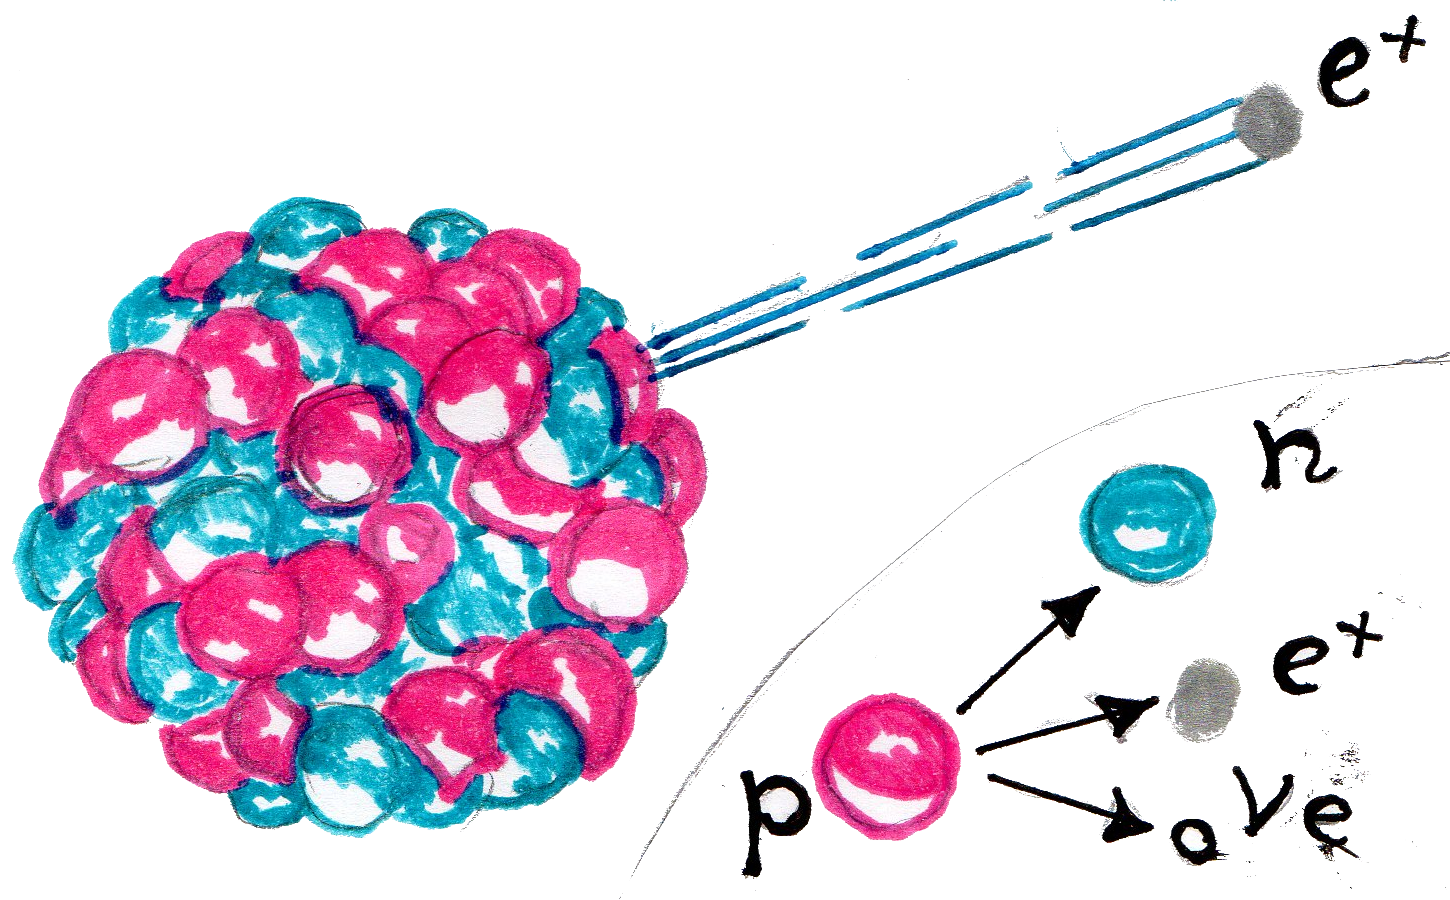
\includegraphics[width=1.0\linewidth]{figures/background_beta_plus_decay.png}
                    
                    \captionsetup{singlelinecheck=false, justification=raggedright}
                    \caption{Graphical example of $\beta+$-decay. Here in the top left of the figure a nucleus can be seen which is unstable as it has an imbalance of protons and neutrons. A positron can be seen exiting the nucleus as a byproduct of $\beta+$-decay converting a proton into a neutron. In the bottom right of the figure a closer example of this can be seen. Here it directly shows a specific proton and the neutron, positron and neutrino which are produced by $\beta+$-decay.} \label{fig:decay_and_annihilation_beta_plus_decay}
                \end{figure}
                
                \begin{figure}
                    \centering
                    
                    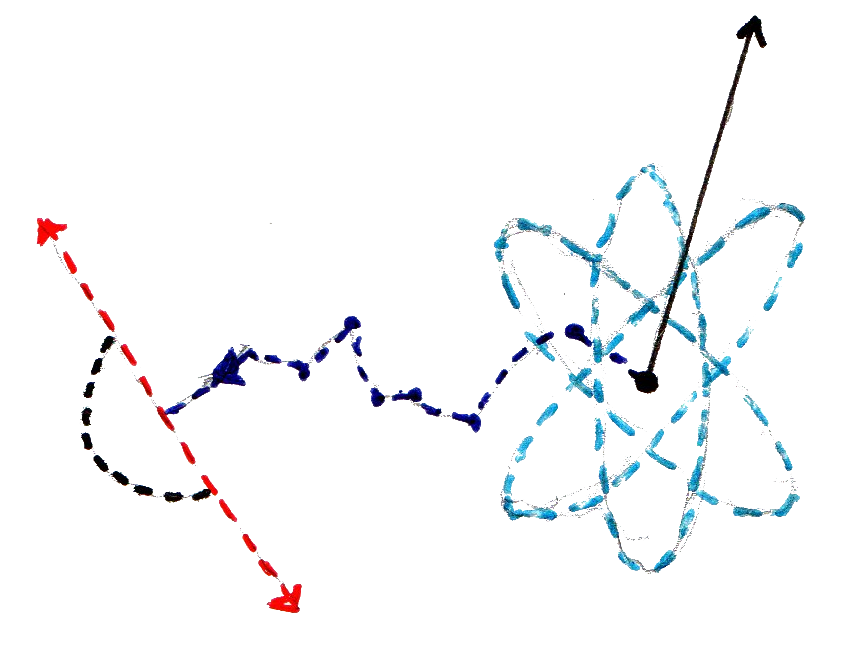
\includegraphics[width=1.0\linewidth]{figures/background_positron_range.png}
                    
                    \captionsetup{singlelinecheck=false, justification=raggedright}
                    \caption{Graphical example of positron range. Here on the right of the figure an atom can be seen travelling with some velocity, a positron is emitted from the nucleus of the atom by $\beta+$-decay. The path that this positron takes can be seen in the centre of the figure represented by a blue line, this path is the positron range. On the left of the figure the annihilation of the positron with an electron occurs and the $\gamma$-photons emitted $\SI{180}{^{\circ}}$ apart are shown.} \label{fig:decay_and_annihilation_positron_range}
                \end{figure}
                
                Radionucleides used in \gls{PET} undergo a type of decay called $\beta+$-decay~\boxcite{conti_beta}. This is due to an instability of the radionuclide, given to an imbalance of neutrons to protons. As a consequence, a proton in its nucleus converts into a neutron releasing a positron and a neutrino, this can be seen in~\Fref{fig:decay_and_annihilation_beta_plus_decay}. The emitted positron travels with some decreasing velocity, from sequential collisions, through the body of the patient, for a distance called positron range, before its final collision and annihilation with its antiparticle the electron, this can be seen in~\Fref{fig:decay_and_annihilation_positron_range}~\boxcite{EvansPositronBib}. %KT citation probably not  needed
                
                The annihilation causes the emission of two $511$ \gls{KeV} $\gamma$-photons at $\SI{180}{^{\circ}}$ apart from one another. However, because the positron-electron pair may not be at rest at the moment of their annihilation, the two emitted photons can show a certain degree of non-collinearity, according to the laws of conservation of momentum. This means that the $\gamma$-photons are almost never exactly $\SI{180}{^{\circ}}$ apart~\boxcite{pet_basic}. %KT I'd cut the last sentence. repetition and you don't want to over-elaborate this
                %, because the positron will usually have a small kinetic energy going into the annihilation. This kinetic energy is conserved after the annihilation as a force in a different direction, usually, to that of the force from the annihilation itself.
                
                A \gls{PET} scanner thus does not image, directly, the emission of the positron but, in fact, more closely images the location of the annihilation. %KT move this sentence down a bit %ACW done
            
            \subsubsection{Static and Dynamic Acquisition} \label{sec:static_and_dynamic_acquisition}
                There are two main types of \gls{PET} scan useful for determining separate processes. These types of scans and uses are:
                
                \begin{itemize}
                    \item The first and most common type of \gls{PET} scan is a static \gls{PET} scan. The patient is scanned only when the injected radiotracer has distributed through their body and eventually spproximately stabilised. %KT ``perfused'' is wrong. I'd say''distributed''. ``consistent'' sounds weird, so I'd say ``eventually approximately stabilised'' %ACW done, thank you
                    The time elapsed between injection and acquisition depends on the half life and metabolisation of the radiotracer. For \gls{F-FDG} about \SI{3600}{\second} is given.
                    
                    \item The second type of \gls{PET} scan is a dynamic scan. The acquisition begins before the radiotracer is injected into the patient. The injection of the radiotracer during the acquisition allows for the kinetics of the tracer to be observed and quantified with the use of compartmental modelling~\boxcite{Lammertsma2017}. For example, from dynamic \gls{PET} \gls{MPI}: %KT cut the ``direct parametric reconstruction'' here. not used in clinical practice. just say ``dynamic PET MPI''
                    in-vivo studies used in conjunction with tracer kinetic modelling enables the quantification of \gls{MBF}, often measured using rubidium $82$. %Radiotracers such as rubidium $82$ are particularly indicated for dynamic scans given their short half life, seen in~\Fref{sec:decay_and_annihilation}. %KT doesn't have anything to do with halflife but with chemistry (calcium analogue). By the way, the ideal ``tracer'' to measure MBF is (radioactive) water! but that needs cycltron on site etc due to very short half-life. In contrast, Rb82 is produced in a generator. so say ``... MBF, often measured using Rb82.'' %ACW done, thank you, i didnt phrase the half life comment well, i mean that none perfusion or dynamic scans would be difficult with it
                \end{itemize}
            
            \subsubsection{PET FOV} \label{sec:pet_fov}
                \begin{figure}
                    \centering
                    
                    \includegraphics[width=1.0\linewidth]{figures/background_total_body_pet.png}
                    
                    \captionsetup{singlelinecheck=false, justification=raggedright}
                    \caption{Graphical representation of the difference between a total body \gls{PET} scanner and a standard \gls{PET} scanner. On the left of the figure a total body \gls{PET} scanner can be seen where the rings of detectors completely engulf the patient. However, on the right of the figure a standard \gls{PET} scanner can be seen where the rings of detectors only cover a portion of the patient. On the case on the right of the figure in order to take a scan over the entire body either individual acquisitions will be needed and concatenated or the bed would have to move while the acquisition was ongoing.} \label{fig:pet_fov_total_body_pet}
                \end{figure}
                
                The \gls{FOV} of the scanner is the area in which it can detect the $\gamma$-photons. Current clinical \gls{PET} scanners, usually, have a cylindrical \gls{FOV} with a length of between \SI{15.0}{\centi\metre} and \SI{25.0}{\centi\metre} and a diameter of between \SI{50.0}{\centi\metre} and \SI{70.0}{\centi\metre}~\boxcite{Pan2019}.
                
                There are multiple ways to acquire data over more than the axial length of scanner, three of these methods are:
                
                \begin{itemize}
                    \item The most simple and widely used method is to take acquisitions over multiple bed positions and concatenate them.
                    
                    \item A method available on some  standard axial length scanners is; to continually move the bed through the rings of the scanner while acquiring data. This is advantageous as it is more comfortable for the patent and provides potentially less movement of the patient. %KT both these advantages can be done with the above step-and-shoot as well. I guess the advantages are patient comfort and potentially less moveemnt of the patient %ACW done
                    A disadvantage of this though is that it introduces another source of motion to the acquisition from moving the bed. This makes standard \gls{MC} much more difficult.
                    
                    \item Alternatively, total body \gls{PET} scanners are becoming more viable for research. %KT let's remove the ``high potential for  clinical applicatoin''. as you note below,price prevents this %ACW done
                    Total body \gls{PET} scanners have an axial \gls{FOV} which contains most of the patients body making multiple acquisitions less necessary while also increasing the sensitivity to detecting annihilations, this can be seen in~\Fref{fig:pet_fov_total_body_pet}~\boxcite{Cherry2018}. However, the increased price and size constitute a limitation.
                \end{itemize}
            
            \subsubsection{Attenuation} \label{sec:attenuation}
                \begin{figure}
                    \centering
                    
                    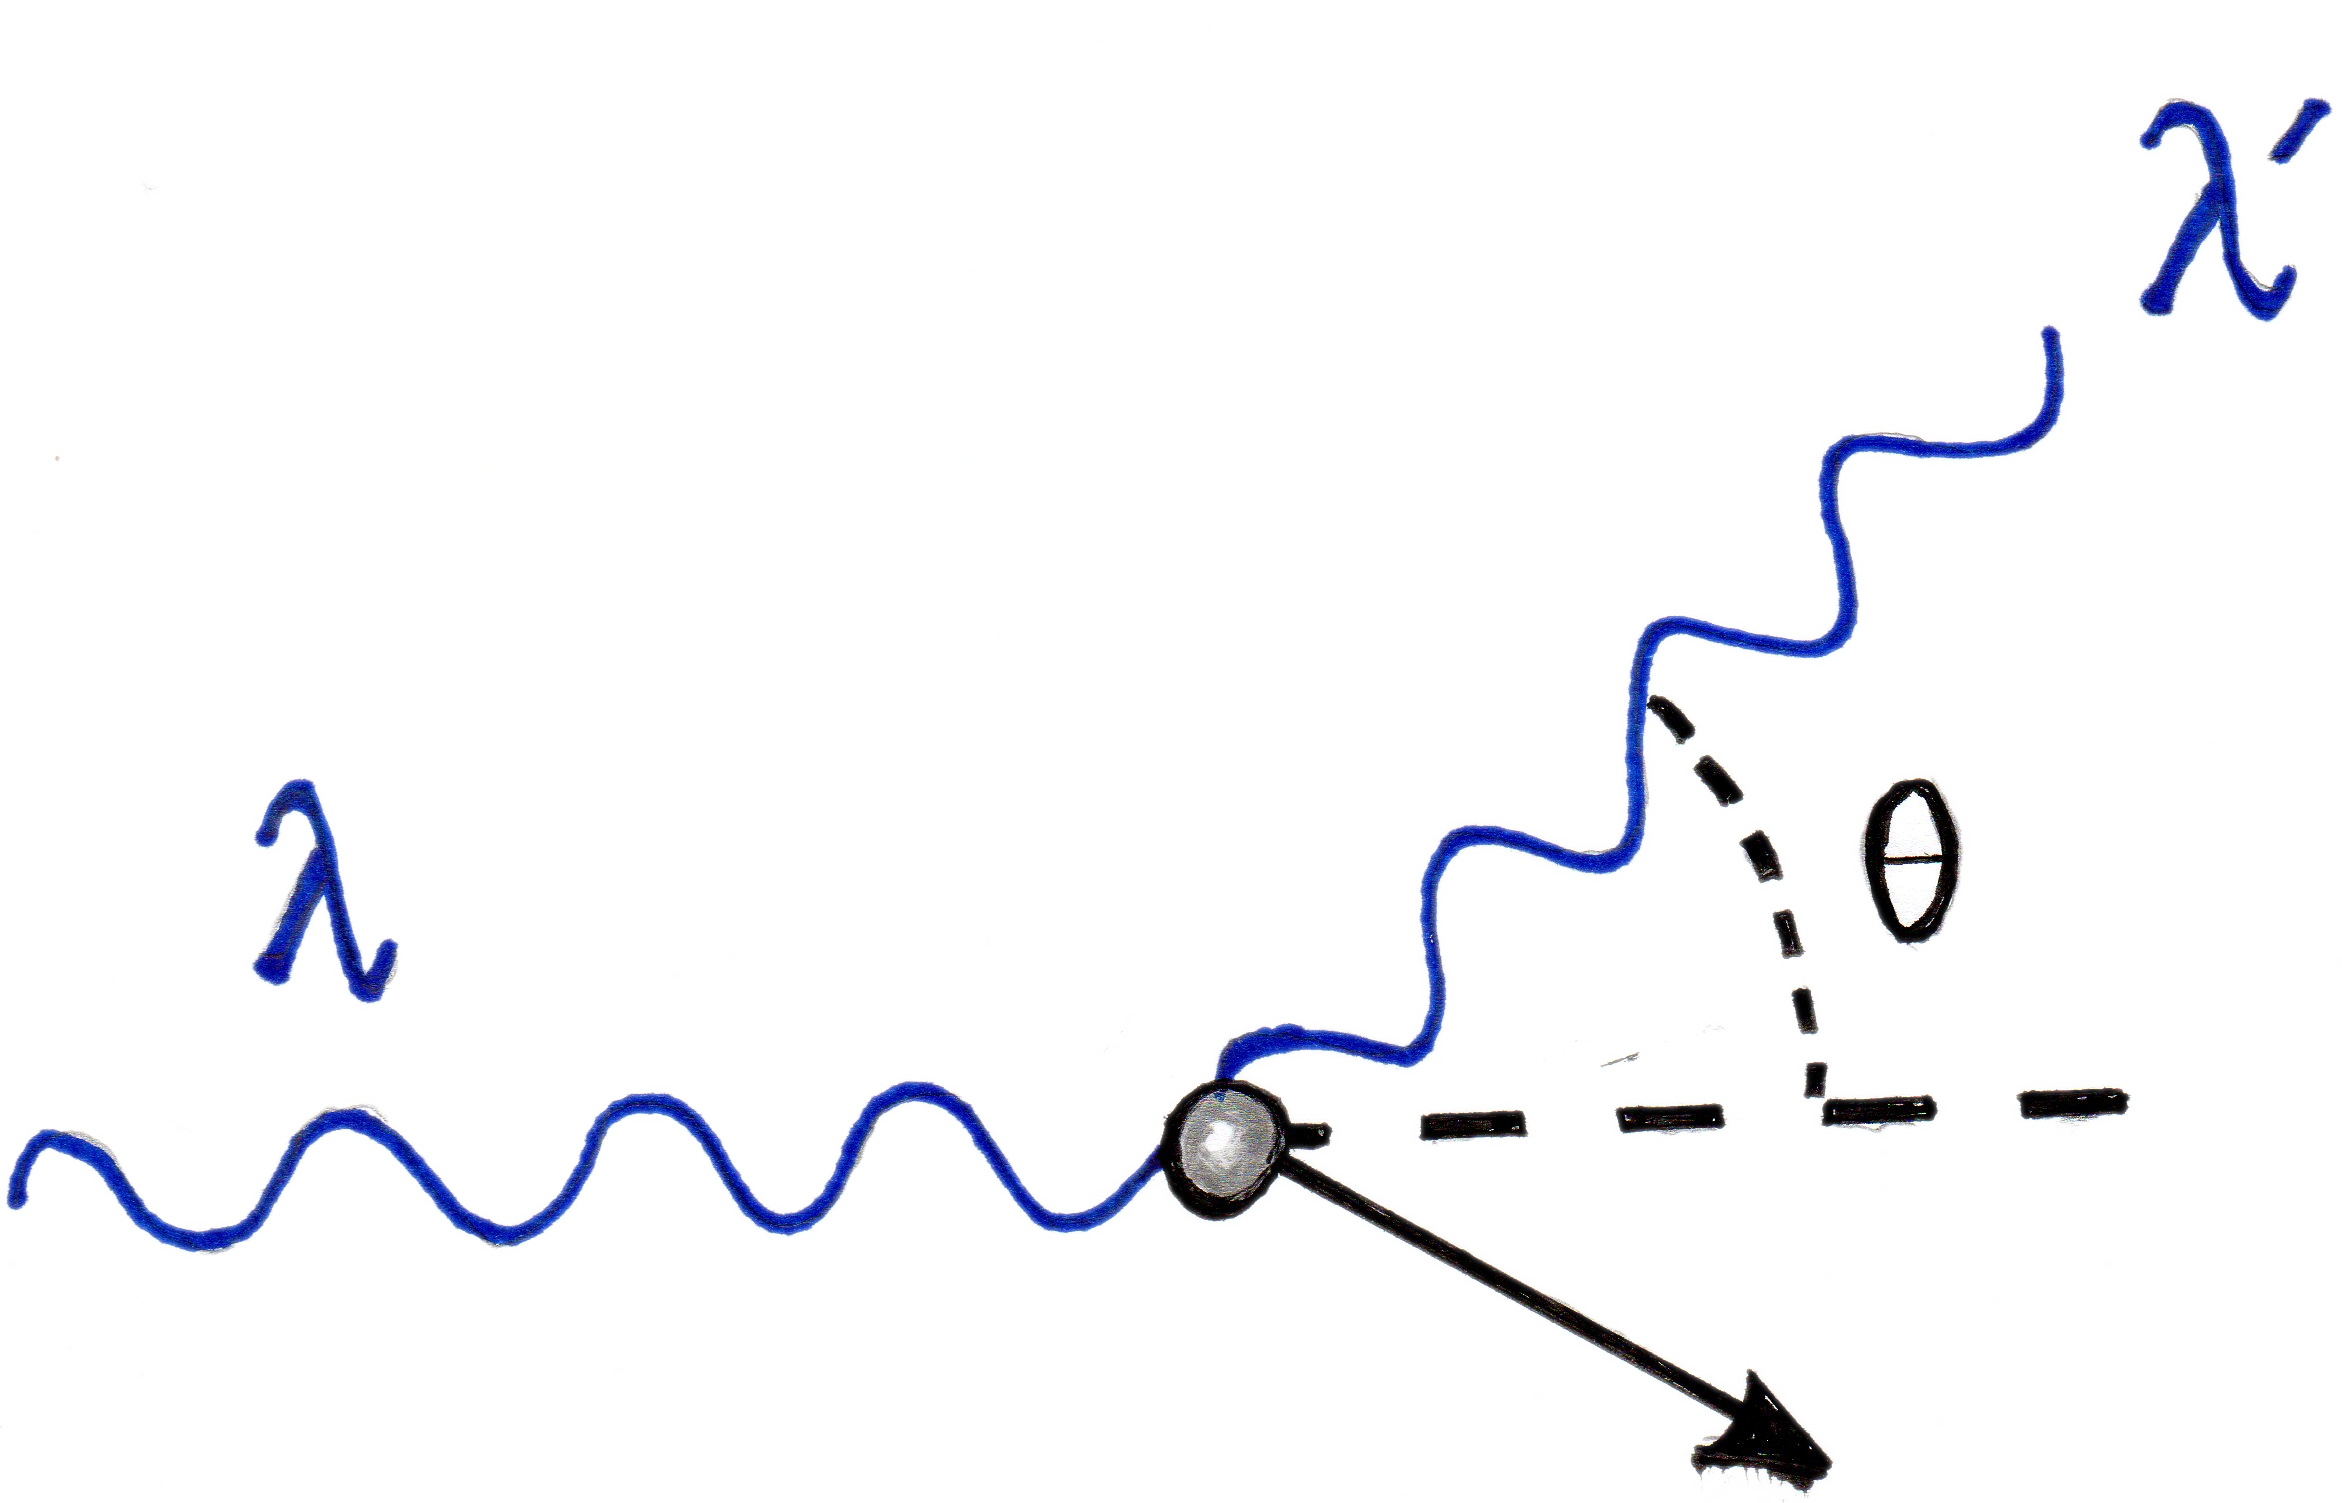
\includegraphics[width=1.0\linewidth]{figures/background_scatter.png}
                    
                    \captionsetup{singlelinecheck=false, justification=raggedright}
                    \caption{Graphical representation of a $\gamma$-photon scattering off of a particle. The $\gamma$-photon can be seen entering the figure on the left hand side before scattering off of a particle in the centre of the figure by an angle $\theta$ and exiting the figure on the top right hand corner. The particle exits the scatter event with some velocity represented by the arrow towards the bottom right. The trajectory of the $\gamma$-photon, had it not been scattered, is shown by the dotted line on the right hand side of the figure.} \label{fig:attenuation_scatter}
                \end{figure}
                
                %KT ``amount of counts'' is not correct. it's a process, or effect, not a number
                %ACW done
                %KT ``who quite literally...'' this doesn't read quite correct.I'd remove that part of the sentence
                %ACW done
                Attenuation is the process or effect through which counts are lost from annihilation to detection by the scanner while the photons are traversing through the body of the patient. Attenuation can amount to a loss of up to \SI{95.0}{\percent} of the total initial signal and can cause increased issues in larger bariatric patients who have more matter that the photons have to pass through increasing the likelihood that they will be scattered or otherwise attenuated~\boxcite{petspringer, Essential2012}. %KT''book'' citation looks strange. missing space in the bibtex? also the guiberteau initials seem strange %ACW done
                
                There are three main ways through which the photon signal can be lost~\boxcite{scienceofpetspringer}, these are in ascending order of magnitude:
                
                \begin{itemize}
                    %KT this isn't a signal loss. I'd cut it (as it doesnt happen in PET)
                    %ACW done
                    %\item Pair production can be thought of as the inverse process compared to annihilation (as discussed above). This is where a subatomic particle and its antiparticle, such as a electron and a positron, are created from a fundamental particle, such as a photon, usually in close proximity to an atomic nucleus. However, because of conservation of energy a photon would need to be of at least $1.022$ \gls{MeV} which is not generally possible for photons created through electron positron annihilation.
                    
                    \item Rayleigh scattering is the elastic scattering of photons without loss of significant energy by particles which are much smaller than the wavelength of the photon. A common example of Rayleigh scattering is the scattering of sunlight in the atmosphere which is causes the blue colour of the sky during the day and the red colour of the sky at sunset. Because the wavelength of $\gamma$-photons is comparably small, compared to most particles, the probability of Rayleigh scattering occurring is negligible and thus it is normally ignored in \gls{PET}.
                    
                    \item Absorption through the photoelectric effect is the process through which the high energy $\gamma$-photon hits and transfers its energy to a material causing the emission of lower energy electrons. The likelihood of the photoelectric effect is inversely proportional to the cube of the photon energy; it also increases as the atomic number of the attenuating material increases. In the matter of the patient the photoelectric effect is most prevalent at photon energies below $100$ \gls{KeV} and as such the probability of the photoelectric effect occurring for the \gls{PET} $\gamma$-photons is minimal~\boxcite{petspringer}. %KT ``here'' say instead ``for the PET gamma photons'' or so. phtoelectirc effect does occur for CT X-rays %ACW done
                    Photoelectric effect occurs mostly in the detectors of the scanner.
                    
                    \item Compton scattering comprises the majority of interactions between the photon and matter in \gls{PET}, it occurs where the photon interacts with an electron in a close by atom. The recoiling electron causes the photon to be deflected along another path transferring energy from photon to electron, this can be seen in~\Fref{fig:attenuation_scatter}. Compton scattering is also known as incoherent scattering because of its effect on the trajectory of the photon. The probability of Compton scattering is indirectly proportional to the energy of the photon~\boxcite{petspringer}.
                \end{itemize}
                
                The relationship between the attenuation of the signal and the material through which it is travelling is given by the Beer-Lambert law. Given $I_0$ incident photons travelling across a path of length $D$, the number of non-scattered photons $\rmI_{\rmD}$ is given by: %KT given all of the above,I recommend to say ``the numberof  non-scattered photons...'' %ACW done
                 
                \begin{equation} \label{sec:eq:beer_lambert_law}
                    \rmI_{\rmD} = \rmI_{0} \cdot \exp\Bigg(\int_{\rmD} - \mu_E(r)\rmd r \Bigg) %KT why := ? %ACW done, because i wanted to be consistent
                \end{equation}

                \noindent where $\mu_E(r)$ is the attenuation coefficient of the media crossed by the photons of energy $E$.
        
        \subsection{Data acquisition} \label{sec:data_acquisition}
            % write a general intro on the scanner structure, and the type of events you detect (true scatter randoms etc)
            
            \begin{figure}
                \centering
                
                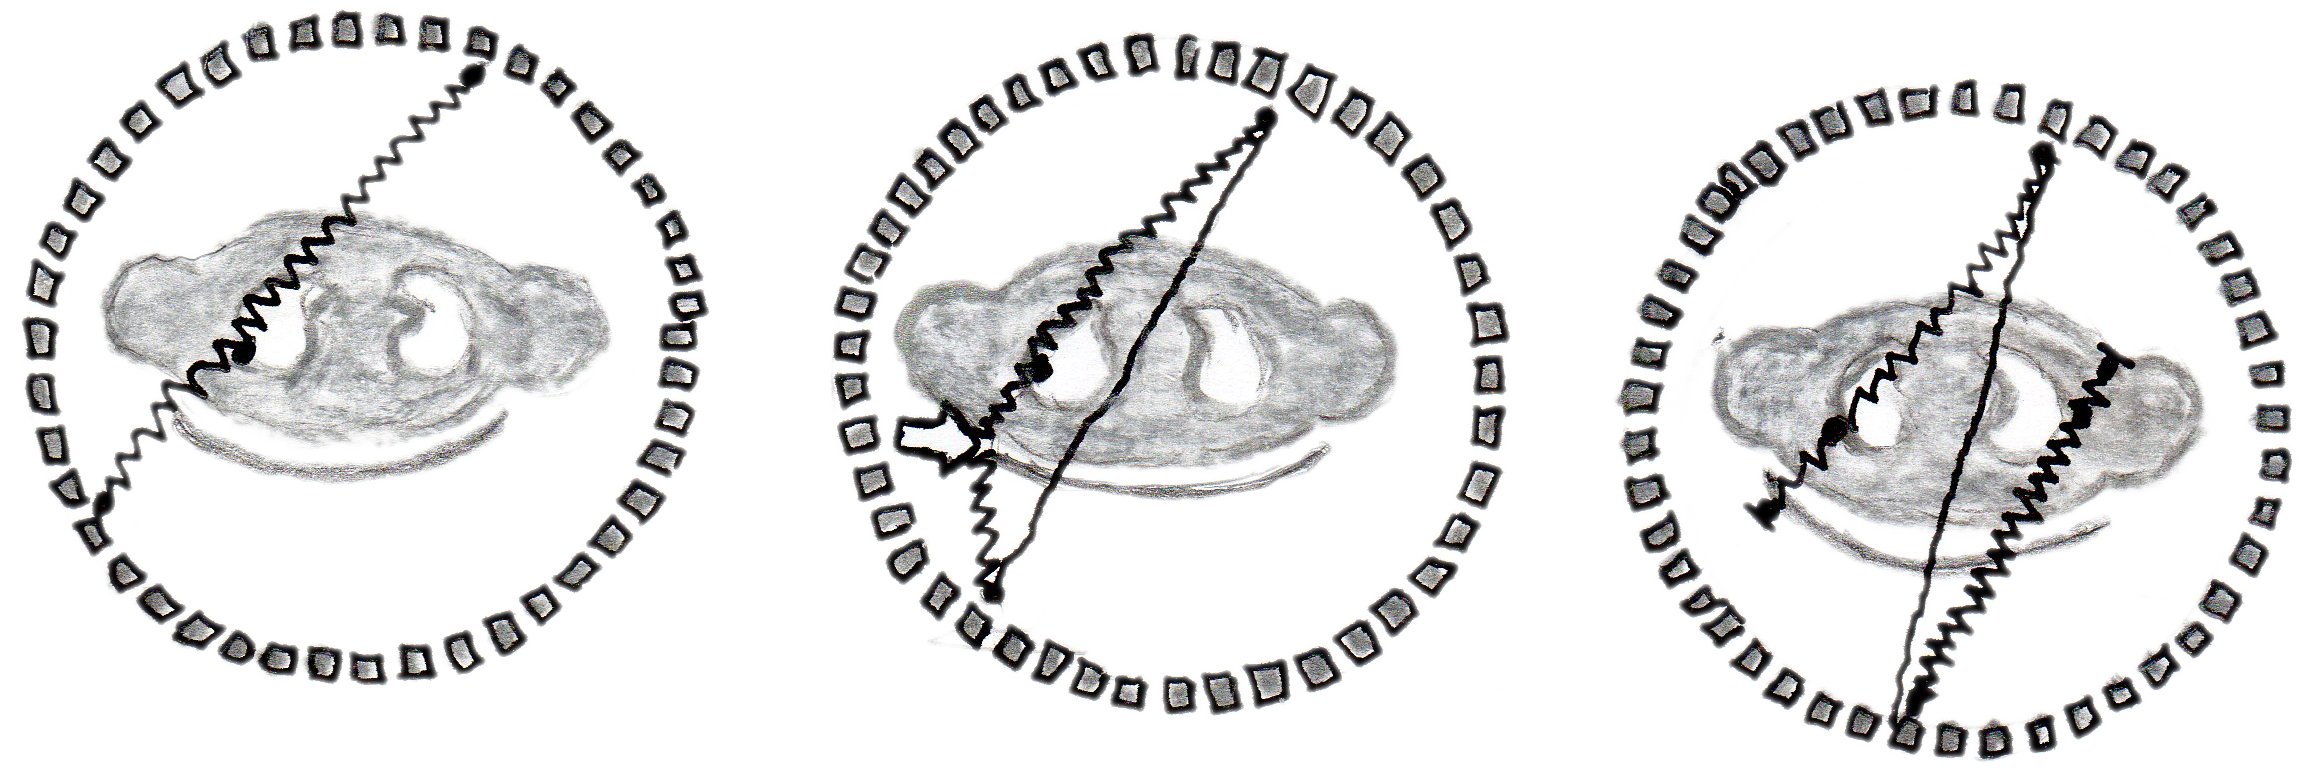
\includegraphics[width=1.0\linewidth]{figures/background_coincidence.png}
                
                \captionsetup{singlelinecheck=false, justification=raggedright}
                \caption{Graphical representation of the different types of coincidences possible in \gls{PET}. On the left of the figure a true coincidence can be seen, this is where the $\gamma$-photons from one annihilation are both detected without scattering. In the middle of the figure a scattered coincidence can be seen, this is where the $\gamma$-photons from one annihilation are both detected, however in this case one of them has scattered. On the right of the figure a random coincidence can be seen, this is where the $\gamma$-photons from two unrelated annihilations are detected.} \label{fig:data_acquisition_coincidence}
            \end{figure}
            
            As discussed in~\Fref{sec:pet_fov}, the structure of a \gls{PET} scanner is that of concentric rings of detectors offset along a central axis. These rings detect each incident photon and attempt to temporally and spatially link opposing photons along a \gls{LOR} through the scanner. A \gls{LOR} being a line through the \gls{FOV} of the scanner linking two detectors. The methods through which the scanner attempts to %detect incident photons and then 
            link relative photons together will be discussed in the following %~\Fref{sec:photon_detection} and
            ~\Fref{sec:coincidence_processing}.
            
            Because of the photons interaction in matter shown in~\Fref{sec:attenuation}, there are four different types of event or coincidences that can be detected by the scanner, these are:
            
            \begin{itemize}
                \item Firstly, the coincidences that originate from the same annihilation event and pass through the body of the patient to the detector without being scattered or attenuated. These coincidences are called true coincidences as they approximately accurately reflect the position of the originating annihilation.
                
                \item Secondly, there are coincidences which may have originated from the same annihilation event but, from which one or more of the incident photons has undergone Compton scattering before detection. These coincidences are called scattered coincidences.
                
                \item Thirdly, there are coincidences where the \gls{LOR} is determined from two photons from two distinct annihilation events, thus the \gls{LOR} does not reflect an actual annihilation in reality. This could occur because one or more of the photons, from the original pair of photons, may have been attenuated or scattered so that it does not arrive at the detector within a reasonable time of its photon pair or that its \gls{LOR} doesn't go through one of the detectors. %KT  much more likely is that its LOR actually doesn't go through one of the detectors! (it's a 3D process of course) %ACW done
                These are called random coincidences.
                
                \item Fourthly, there could be a situation where three or more photons are detected within close temporal proximity to one another. Because of the close time of detection, in this case it is not possible to determine which photons reflect an actual annihilation and which are random coincidences. These coincidences are called multiple coincidences. In normal procedures this is rare. %KT I recommend say that this is in normal procedures  rare. Otherwise an obvious viva question would be what people would do with them (as they're not in your equation below) %ACW done
            \end{itemize}
            
            An example of some of the types of coincidences from above can be seen in~\Fref{fig:data_acquisition_coincidence}.
            
            The total prompts detected during a \gls{PET} acquisition $P$ can be expressed as:
            
            \begin{equation}
                P := T + S + R
            \end{equation}
            
            \noindent where $T$ is the number of true coincidences, $S$ is the number of scattered coincidences and $R$ is the number of random coincidences. %Thus the usual total sum of scattered and random coincidences when compared to true coincidences is a ratio of $2$ to $1$. %KT this last sentence is incorrect. depends on count-rate, amount of scatter etc etc. Delete it %ACW done
            
%            \subsubsection{2D and 3D Acquisition} \label{sec:2d_and_3d_acquisition}
                %KT the 2D stuff reads as if in 2D PET there were collimators between all detectors, but in fact they were only between rings.
                %I highly recommend cutting this subsubsection. Detail not relevant to your work.
                %ACW depressingly done
%                \begin{figure}
%                    \centering
                    
%                    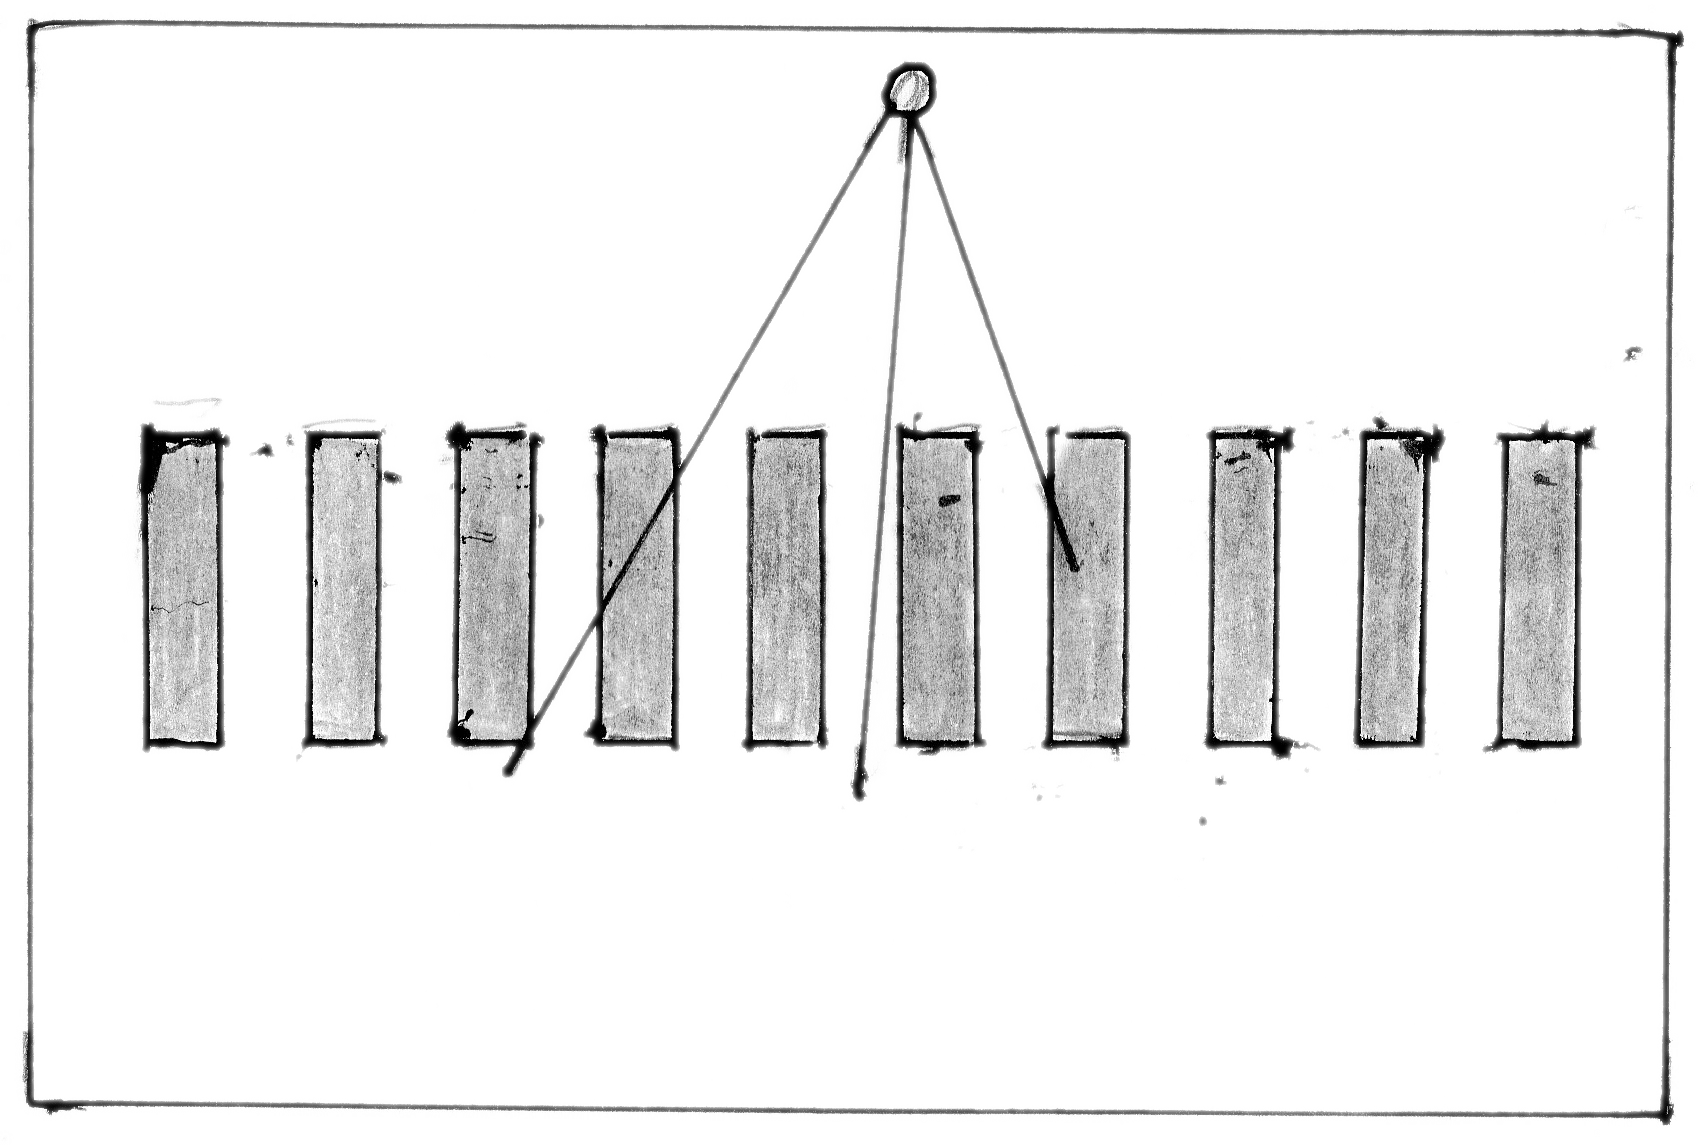
\includegraphics[width=1.0\linewidth]{figures/background_septa.png}
                    
%                    \captionsetup{singlelinecheck=false, justification=raggedright}
%                    \caption{Graphical representation of the cross section of the septa used for collimation in \gls{2D} \gls{PET} acquisitions. In this figure a point can be shown casting paths into the slits of the septa, as can be seen the paths from the point can only pass through the slits of the septa in positions where the angle of the line with respect the the walls of the septa is acute.} \label{fig:2d_and_3d_acquisition_septa}
%                \end{figure}
                
%                There are two different methods used in \gls{PET} to determine or constrain to be certain of the spatial position or angle of the \gls{LOR} along the axis of the scanner, these are:
                
%                \begin{itemize}
%                    \item The method which was used for a long time in other applications (such as \gls{SPECT}) and until recently in \gls{PET} was; to place a block of, usually, tungsten metal (for its photon absorbing properties) in front of all of the detectors, this block is called s septa, this can be seen in~\Fref{fig:2d_and_3d_acquisition_septa}. The septa has very small slits cut into it which would only allow photons to pass through which entered the slits at an acute angle. Thus the septa constrains the photons to being almost perpendicular to the detector (on axis) and as such each detector only receives signal from annihilations that occur within its ring. This process is called collimation and the subsequent acquisition is called a \gls{2D} acquisition, \gls{2D} not because it results in a single image but because it is comprised of distinct \gls{2D} projections.
                    
%                    \item The more modern method is to simply remove the septa from the scanner and to record coincidences between all rings. This is significantly more computationally expensive than a \gls{2D} acquisition but it also increases the sensitivity of the scanner meaning that scanning times can be reduced. Because this method produces projections between all rings it is known as a \gls{3D} acquisition~\boxcite{Schmitz2013}.
%                \end{itemize}
            
%            \subsubsection{Photon Detection} \label{sec:photon_detection}
                %KT I did not read this. Far far too much detail for your thesis. I highly recommend commenting it out
                %ACW depressingly done
%                \begin{figure}
%                    \centering
                    
%                    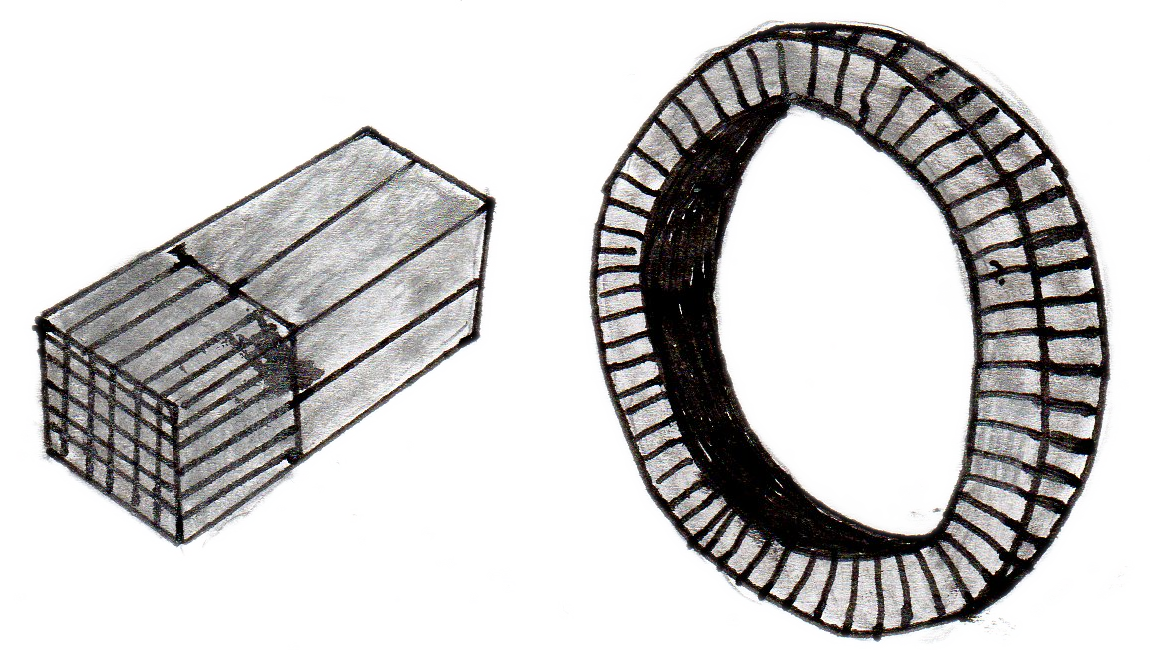
\includegraphics[width=1.0\linewidth]{figures/background_detector.png}
                    
%                    \captionsetup{singlelinecheck=false, justification=raggedright}
%                    \caption{Graphical representation of the block detector structure of the scintillator crystal and the photodetector (with multiple scintillator crystals per photodetector), on the left of the figure, and an example of how these block detectors would be combined to construct a ring of a \gls{PET} scanner, on the right of this figure.} \label{fig:photon_detection_detector}
%                \end{figure}
                
%                \begin{figure}
%                    \centering
                    
%                    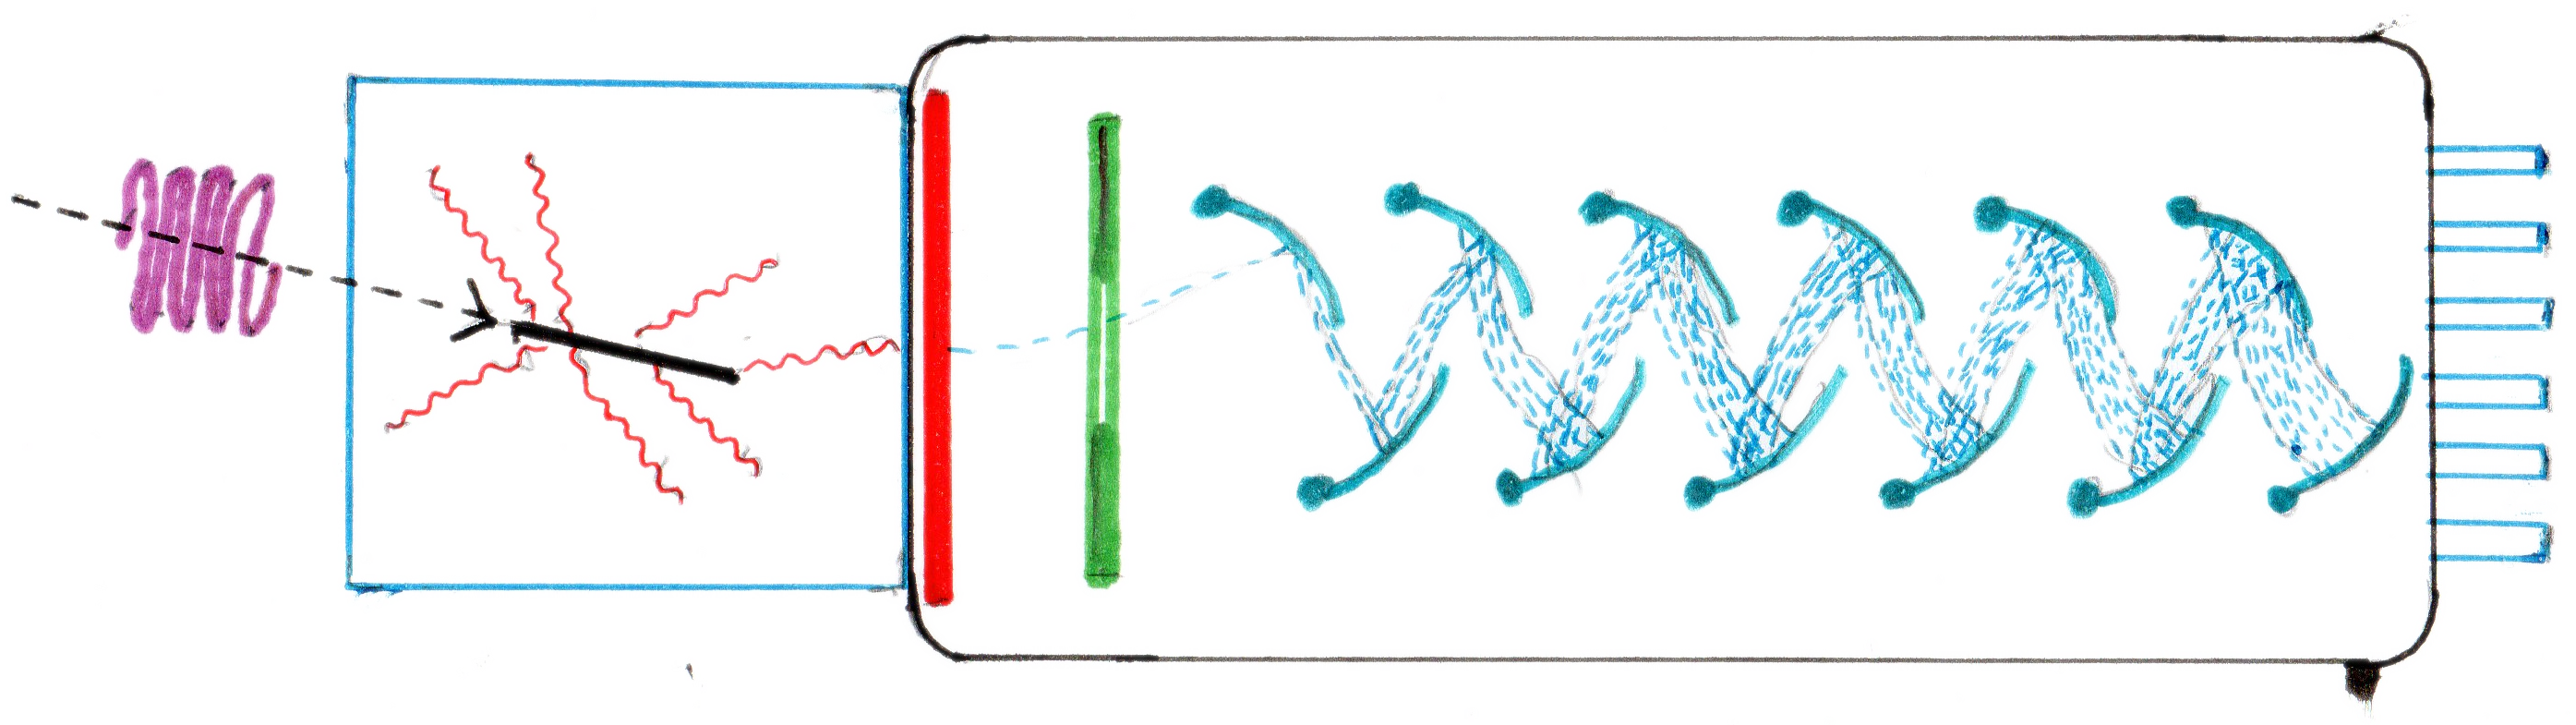
\includegraphics[width=1.0\linewidth]{figures/background_photomultiplier.png}
                    
%                    \captionsetup{singlelinecheck=false, justification=raggedright}
%                    \caption{Graphical representation of a scintillator crystal coupled to a \gls{PMT}. On the left of this figure a photon can be seen impinging upon the scintillator crystal and then being attenuated by the photoelectric effect at some depth. The electrons produced by this can then be seen, in the centre of this figure, interacting with the photocathode before being focused onto the first dynode. On the right of this figure, a naive representation, the amplification of the electrons can be seen by subsequent dynodes.} \label{fig:photon_detection_photomultiplier}
%                \end{figure}
                
%                PET detectors consist of two main components; a scintillator crystal, which, partially because of the photoelectric effect, when exposed to ionising radiation produces visible light through luminescence, and a photodetector or photomultiplier which amplifies the intensity of an input light similarly to how a vacuum tube or a transistor would amplify an electrical signal. These can be seen in~\Fref{fig:photon_detection_detector}.
                
%                For use in \gls{PET} the following properties are desirable for a scintillator crystal:
                
%                \begin{itemize}
%                    \item Firstly, the crystal should have a high stopping power. This means that the photon does not travel a great distance into the crystal before it undergoes attenuation by the photoelectric effect. Usually the higher the density of the scintillator crystal the greater the stopping power.
                    
%                    \item Secondly, for each incident photon the scintillator should have a high light output. This not only means that the work photomultiplier will have to amplify the output less but it also means that discriminating between scattered and unscattered photons will be easier as the discrepancy between the output intensity of the two will be greater.

%                    \item Thirdly, the scintillator should return to a state where it can luminesce again rapidly after each incident photon. This means that more photons can be detected over time and that the exact moment a photon is attenuated can be better measured.
                    
%                    \item Finally, a scintillator crystal should not be hygroscopic. To be hygroscopic means that something has a tendency to absorb water.
%                \end{itemize}
                
%                The first \gls{PET} scanners used \gls{NaI} scintillator crystals before moving to \gls{BGO} and then to \gls{LSO} and \gls{LYSO}. Each new generation of scintillator crystals provided a different balance of the above characteristics. \gls{LSO} and \gls{LYSO} have the best combination of efficiency and time resolution while not being hygroscopic~\boxcite{BGOCherenkovBib, ScintilatorsBib, Mao2013CrystalCrystals}.
                
%                There are three main types of photodetector or photomultiplier, these are:
                
%                \begin{itemize}
%                    \item The first kind of photodetector to be used in \gls{PET} was the \gls{PMT}, this device functions using an initial photocathode and a focusing electrode which takes the output from the scintillator and directs it towards a chain of dynodes. Dynodes are an intermediate electrode which when struck by a photoelectron emit more photoelectrons at a more positive electrical potential through secondary emission. Each subsequent dynode is a a higher potential and emits more photoelectrons than the last causing the input signal to be amplified, this can be seen in~\Fref{fig:photon_detection_photomultiplier}. Some disadvantages of \gls{PMT} are that they are relatively bulky, are effected by a magnetic field and have a relatively low efficiency at approximately \SI{25.0}{\percent}~\boxcite{petspringer, SiPmBib}.
                    
%                    \item To attempt to combat the low efficiency mentioned above the \gls{APD} was developed, this device utilises a semiconductor where there is a junction between positive and negative type silicone, this is similar to a traditional diode. This allows for efficiencies approaching \SI{85.0}{\percent}, they are much smaller than \gls{PMT} and are safe to be used in a magnetic field. However, this also comes with the drawbacks that \gls{APD} produces so much heat that it requires an active cooling system and exhibits worse timing characteristics than the \gls{PMT}~\boxcite{AvalanchePhotodiodeBib}. \gls{APD} is the choice of many modern \gls{PET}/\gls{CT} scanners~\boxcite{Vandendriessche2019}.
                    
%                    \item A further development on \gls{APD} gave \gls{SiPM} and \gls{SSPM}. These devices combine the benefits of both \gls{PMT} and \gls{APD} in that they have a high efficiency, small size, are safe to be used in a magnetic field and have good timing characteristic. \gls{SiPM} and \gls{SSPM} are becoming the new default photodetectors in \gls{GE} scanners~\boxcite{SiPmBib}.
%                \end{itemize}
            
            \subsubsection{Coincidence Processing} \label{sec:coincidence_processing}
                % write stuff about coincidence processing , give some info on TOF (or separate section for it, i don't know)
                
                \begin{figure}
                    \centering
                    
                    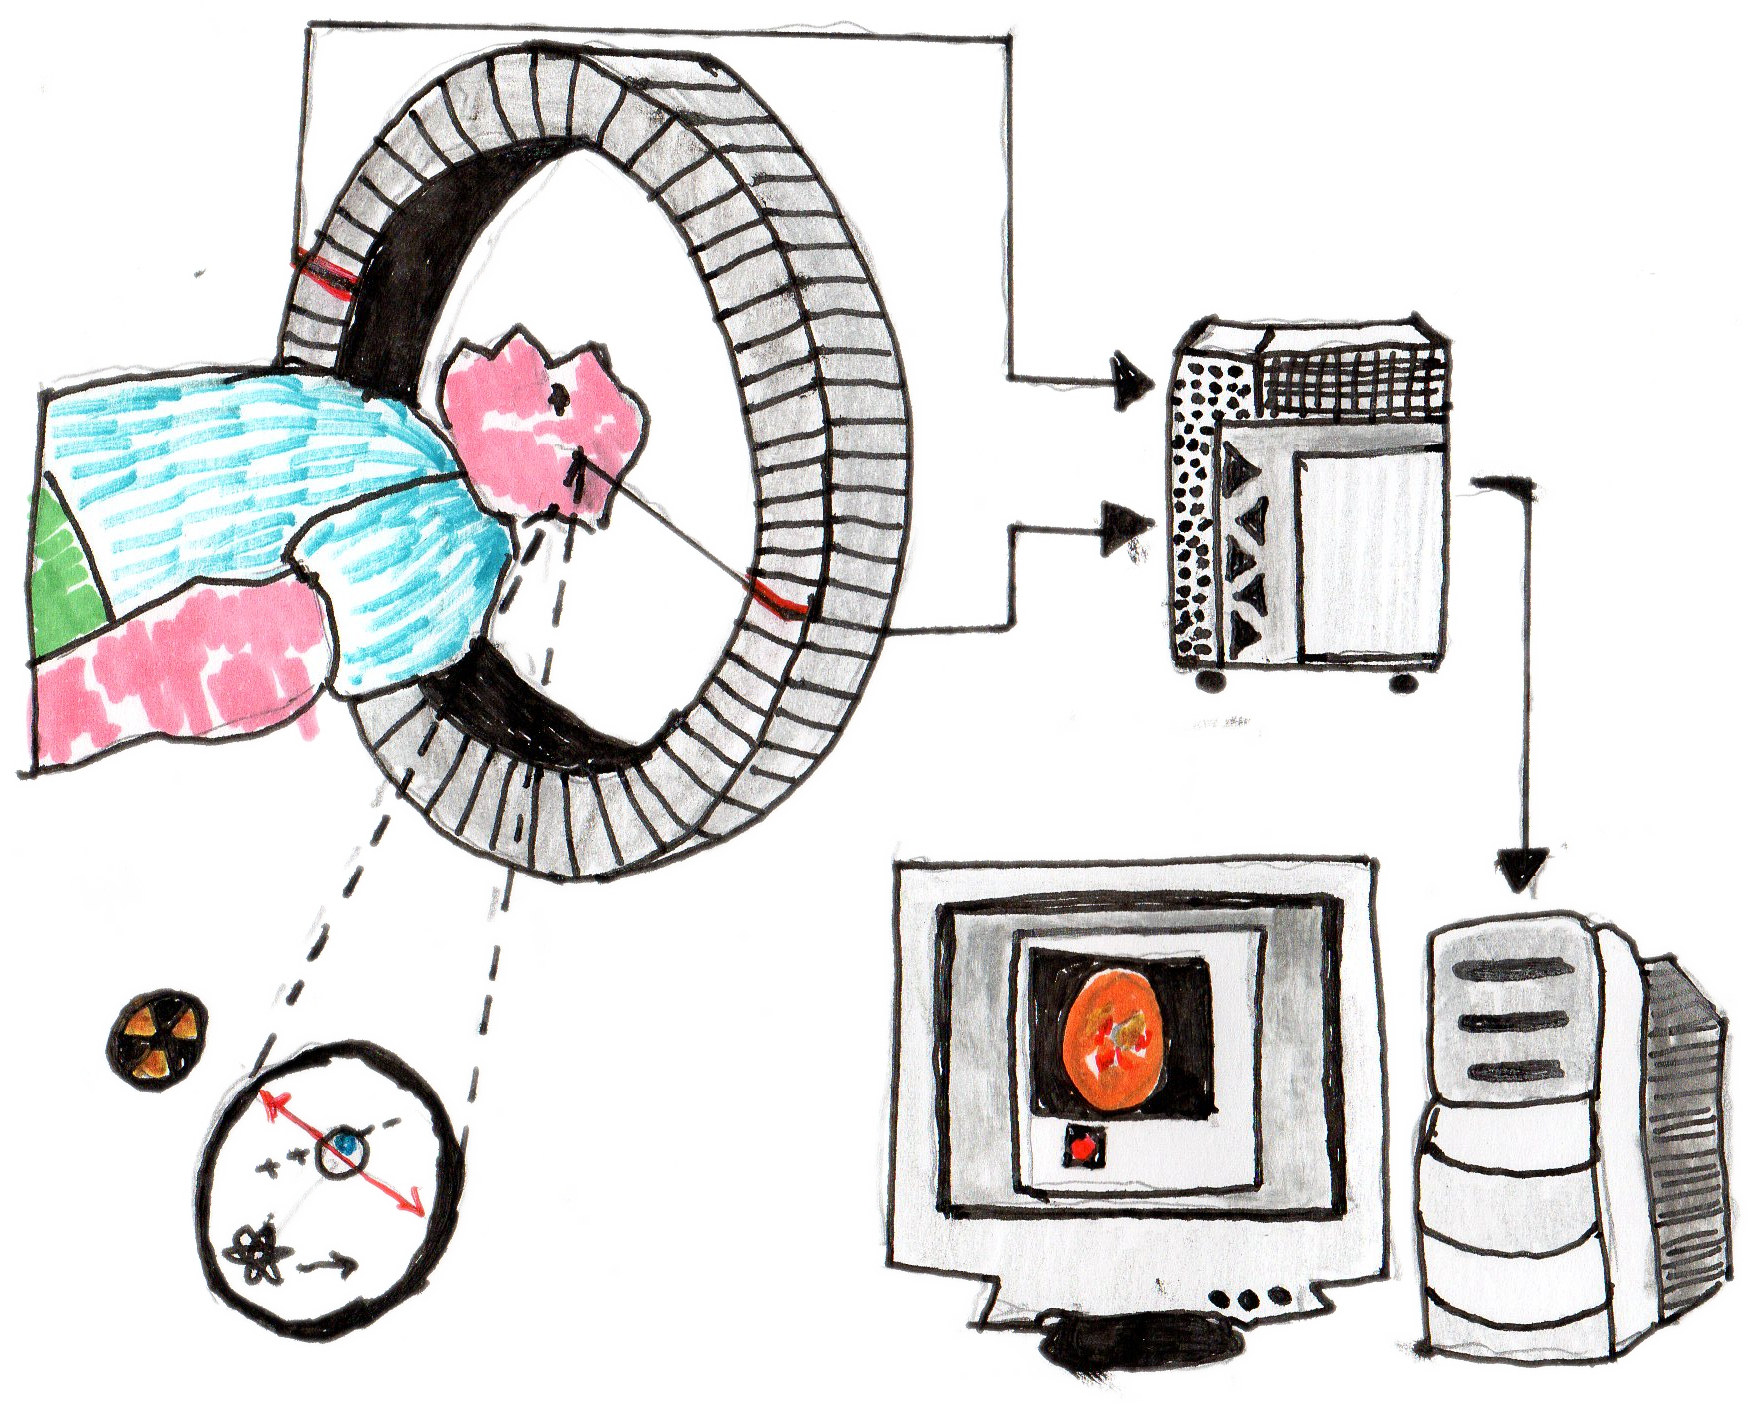
\includegraphics[width=1.0\linewidth]{figures/background_coincidence_processing.png}
                    
                    \captionsetup{singlelinecheck=false, justification=raggedright}
                    \caption{Graphical representation of the workflow from annihilation, to physical detection by the scanner, to then coincidence processing by the electronics of the scanner, before finally displaying some output to the user.} \label{fig:coincidence_processing_coincidence_processing}
                \end{figure}

                %KT first sentence sounds a bit weird. what does an LOR have to do with this? I'd shorten it.
                %ACW done
                %In order for a \gls{LOR} to be determined, the annihilation from which pairs of detected photons come from must be determined, in other words, they must be paired together in some way, as briefly mentioned above in~\Fref{sec:data_acquisition}.
                In order to form coincidences, the incident photons must be paired together to an annihilation event. First, before forming coincidences, the photons are filtered by selecting ones which only fall within an energy window of the scanner, for the \gls{GE} Discovery 690/710 \gls{PET}/\gls{CT} this energy window fall approximately between $425$ and $600$ \gls{KeV}~\boxcite{Bettinardi2011}. Additionally, to attempt to determine temporally if two detected photons belong to the same annihilation event a coincidence window is used. If the events arrive more than the time of the coincidence window apart then they are determined to be unrelated. A standard coincidence window size would be about \SI{5.0}{\nano\second}. A naive representation of the workflow for coincidence processing can be seen in~\Fref{fig:coincidence_processing_coincidence_processing}.
            
            \subsubsection{Time of Flight PET} \label{sec:time_of_flight_pet}
                \begin{figure}
                    \centering
                    
                    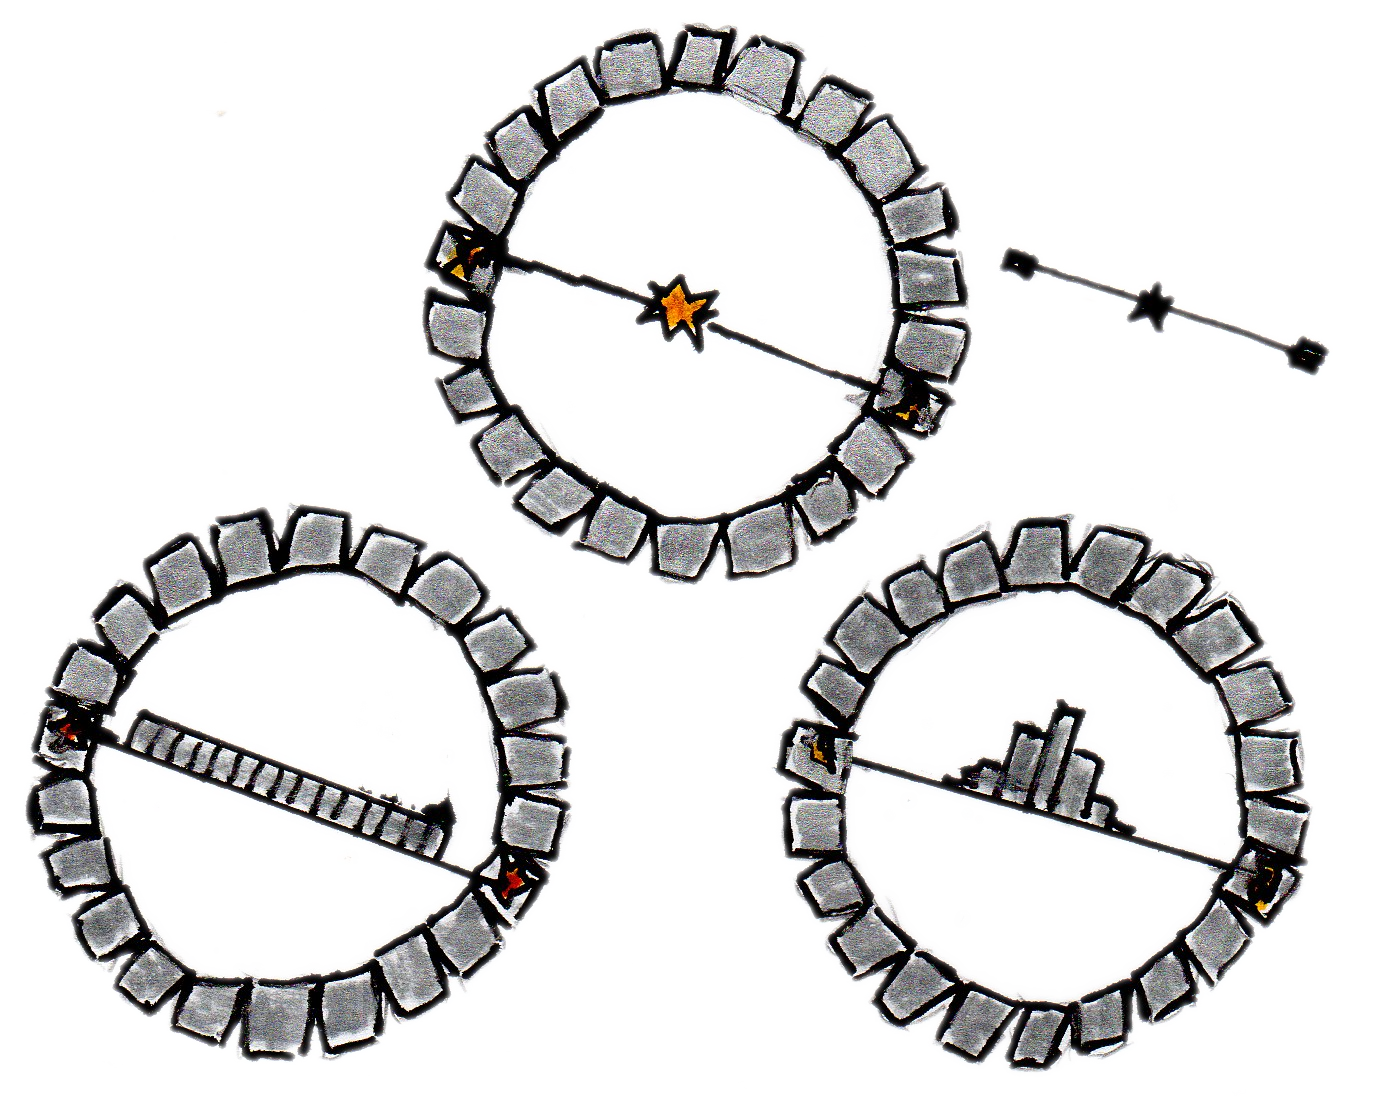
\includegraphics[width=1.0\linewidth]{figures/background_tof.png}
                    
                    \captionsetup{singlelinecheck=false, justification=raggedright}
                    \caption{Graphical representation of the concept of \gls{TOF}. The top middle of this figure shows the position where a hypothetical annihilation has occurred, plus the $\gamma$-photos from this annihilation which have then gone on to be detected by the scanner. The bottom left of this figure shows a traditional \gls{NTOF} acquisition where the probability of the position of the annihilation along the \gls{LOR} is constant. The bottom right of this figure shows a \gls{TOF} acquisition where the probability of the position of the annihilation along the \gls{LOR} can be approximated with a Gaussian based upon the difference in arrival time of both photons.} \label{fig:time_of_flight_pet_tof}
                \end{figure}
                
                \begin{figure}
                    \centering
                    
                    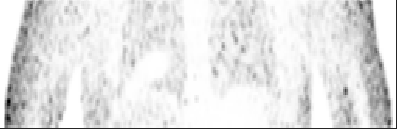
\includegraphics[width=1.0\linewidth]{figures/background_non_tof_example.png}
                    
                    \captionsetup{singlelinecheck=false, justification=raggedright}
                    \caption{Example of some \gls{NAC} \gls{NTOF} data, with noise, with no motion, randoms or scatters, of the thorax with a spherical lesion in the lungs. Coronal view.} \label{fig:time_of_flight_pet_non_tof_example}
                \end{figure}
                
                \begin{figure}
                    \centering
                    
                    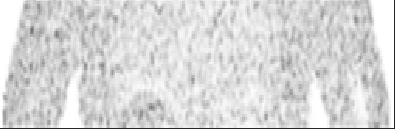
\includegraphics[width=1.0\linewidth]{figures/background_tof_example.png}
                    
                    \captionsetup{singlelinecheck=false, justification=raggedright}
                    \caption{Example of some \gls{NAC} \gls{TOF} data, with noise, with no motion, randoms or scatters, of the thorax with a spherical lesion in the lungs. Coronal view.} \label{fig:time_of_flight_pet_tof_example}
                \end{figure}
                
                As stated above in~\Fref{sec:coincidence_processing}, in order for the coincidence window based method to determine which specific detected photons represent \gls{LOR}, the scanner must be able to asses the difference in arrival time of each photon. %Because of this the scanner must record the absolute time at which it detects each incident photon. %KT delete previous sentence. it isn't really  necessary and essentially irrelevant anyway %ACW done
                It had been hypothesised for some time (since the 1960s) that given the speed of light and the difference in arrival time at each detector, for each photon that makes a specific \gls{LOR}, then it should be possible to approximately calculate the position upon the \gls{LOR} at which a given annihilation occurred. %, known as \gls{TOF}. %KT ``know as TOF'' doesn't flow with the rest of the sentence %ACW done
                This can be seen in~\Fref{fig:time_of_flight_pet_tof}~\boxcite{Surti2015, TOFPhotodetectorsBib}.
                
                The reason for the uncertainty of the position along the \gls{LOR} is because of the relatively course timing resolution of each given scanner. Generally modern \gls{PET}/\gls{CT} scanners have a timing resolution ranging between \SI{200.0}{\pico\second} and \SI{600.0}{\pico\second}, which represents an approximate spatial uncertainty of between \SI{30.0}{\milli\metre} and \SI{90.0}{\milli\metre}. %KT I think you forgot to divide by 2 %ACW done
                The uncertainty within these \gls{TOF} bins is usually modelled using a Gaussian distribution centred around the estimated position of annihilation by the scanner.
                
                %KT cut next paragraph. too much detail for you
                %ACW depressingly done
                %The timing resolution of the scanner is mainly dictated by the timing properties of both the scintillation crystal and the photodetector used. For the scintillation crystal, almost ubiquitously \gls{LSO} and \gls{LYSO} are used in modern \gls{PET} scanners which utilise \gls{TOF}. This is because they are the only scintillation crystals where they stop the photon and return to their base state post luminescence in a suitable time such that the time of arrival can be determined to any useful degree~\boxcite{TOFLSOBib}. For the photodetector, though \gls{PMT} possessed suitable timing properties to be used for \gls{TOF} now \gls{SiPM} and \gls{SSPM} are suppassing \gls{PMT} both in their timing properties and because they are not affected by magnetic fields and such can be used in both \gls{PET}/\gls{CT} as well as \gls{PET}/\gls{MR} scanners.
                
                Currently, \gls{TOF} is a focus for research because of the drastic improvements that it can have on the \gls{SNR}~\boxcite{Lecoq2017, Cates2018}. %\gls{TOF} has such an impact on the resolution and reconstruction of \gls{PET} that it is used as a pseudo attenuation correction technique outside of the \gls{FOV} of the \gls{MR} in some \gls{PET}/\gls{MR} systems, such as the \gls{GE} Signa~\boxcite{Pan2019}. %KT I'd cut the previous sentence. This is  far more complicated than this (needs MLAA etc) %ACW done
                An example of some \gls{NAC} \gls{NTOF} and \gls{NAC} \gls{TOF} data can be seen in~\Fref{fig:time_of_flight_pet_non_tof_example} and~\Fref{fig:time_of_flight_pet_tof_example} respectively, notice the difference in distribution of counts in the centre of the thorax and lungs.
                
                The \gls{PET}/\gls{CT} scanner with the highest \gls{TOF} resolution which is commercially available is the Siemens Vision with an approximate \gls{FWHM} of \SI{210.0}{\pico\second} or \SI{31.5}{\milli\metre}~\boxcite{VanSluis2019}. The \gls{PET}/\gls{MR} scanner with the highest \gls{TOF} resolution which is commercially available is the \gls{GE} Signa with an approximate \gls{FWHM} that is sub \SI{400.0}{\pico\second} or \SI{60.0}{\milli\metre}~\boxcite{SIGNA, Hsu2017StudiesSystem, Grant2016NEMASystem, Caribe2019NEMAIsotopes}. %KT again factor 2in the mm %ACW done
            
            \subsubsection{Data Output} \label{sec:data_output}
                \begin{figure}
                    \centering
                    
                    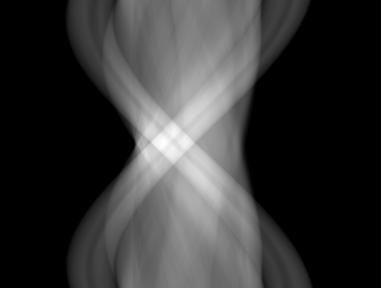
\includegraphics[width=1.0\linewidth]{figures/background_sinogram_data_example.png}
                    
                    \captionsetup{singlelinecheck=false, justification=raggedright}
                    \caption{Example of some simulated sinogram data, with no motion, noise, randoms or scatters, of the thorax with a spherical lesion in one of the lung.} \label{fig:data_output_sinogram_data_example}
                \end{figure}
                
                \begin{figure}
                    \centering
                    
                    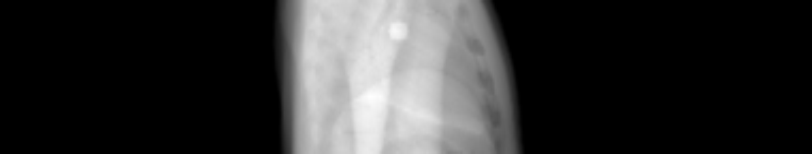
\includegraphics[width=1.0\linewidth]{figures/background_viewgram_data_example.png}
                    
                    \captionsetup{singlelinecheck=false, justification=raggedright}
                    \caption{Example of some simulated viewgram data, with no motion, noise, randoms or scatters, of the thorax with a spherical lesion in one of the lung.} \label{fig:data_output_viewgram_data_example} %KT fine, but it hardly shows what it's a sinogram (as you used a viewgram). maybe show both? %ACW done
                \end{figure}
                
                The output from a \gls{PET} scanner must be stored in a %universally understood
                file format in order to be of any use. %KT not true (in theory, but also not in practice. As long as the manfacturer can read it, they're fine...) %ACW done
                This file format will usually contain information related to the prompts from the acquisition, discussed above in~\Fref{sec:data_acquisition}. Each prompt stored represents a \gls{LOR} connecting the centre of two detectors. %KT probably first time you define LOR, while used multiple times above %ACW done
                Where \gls{TOF} information is available it is stored as an extra dimension in this file. This file can then be taken and reconstructed in order to estimate the original distribution of the radiotracer in the patient, this will be discussed later in~\Fref{sec:pet_image_reconstruction}.
                
                There are two main formats in which this information is stored from the scanner:
                
                \begin{itemize}
                    \item The most common way, that is used in clinical practise, is a format called a sinogram. During acquisition, if a sinogram output is specified, then the coincidences detected by the scanner are binned into a histogram which represents their plane orthogonal to the scanner, their orientation angle, their average axial location and their distance from the centre of the gantry. \gls{TOF} can be added as an additional dimension if it is used. %KT and TOF... %ACW done
                    If a single point source were imaged it would produce a sinusoid when binned into a sinogram, hence the name. An example of some siogram and viewgram data, with no noise, can be seen in~\Fref{fig:data_output_sinogram_data_example} and~~\Fref{fig:data_output_viewgram_data_example} respectively. Because data is being binned into a histogram with this method,  information is lost, it could be considered a lossy compression method.
                    
                    \item A less common method but one which is becoming more prevalent is a format called listmode data. Here each coincidence is recorded sequentially in a file. The information stored for each coincidence includes its arrival time, the coordinates of the detector and its detected energy. \gls{TOF} information can also be stored if it is used. %KT what do you mean with ``and coincidence''. don't forget TOF info... %ACW done
                    A listmode file can be directly reconstructed or first unlisted into a sinogram post acquisition. %Because a listmode file does not compress the output from the scanner, such as by binning the data into a histogram like with a sinogram, then the size of a listmode file will always be inherently larger than an equivalent sinogram. %KT cut previous sentence. it's not correct because of 2 reasons. If you have only 2 counts, the listmode file will be shorter. Siemens does compress info in the listmode file (to save space) %ACW done
                \end{itemize}
            
            \subsubsection{PET resolution} \label{sec:pet_resolution}
                There are five main effects which impact the resolution of a \gls{PET} acquisition, these are:
                
                \begin{itemize}
                    \item Firstly, there is, as has been discussed above in~\Fref{sec:decay_and_annihilation}, the effect of positron range. Because the positron travels a small distance before annihilating the \gls{PET} scanner will always, at best, be measuring the position of the annihilation rather than the position of the decay and as such not directly measuring the position of the radiotracer~\boxcite{PositronRangeLevinHoffmanBib}.

                    %KT ``as discussed''. exactly. so cut most of the remaining text!
                    %ACW done
                    \item Secondly, again as discussed above in~\Fref{sec:attenuation}, acolinearity of the $\gamma$-photons introduces errors which affect the resolution of \gls{PET}. %because the positron will almost always enter the annihilation event with some velocity then the $\gamma$-photons produced will exit with the same additional velocity. This velocity is also almost always in a direction other than that which the $\gamma$-photon would otherwise travel in, this causes the photons to travel in a direction which is not exactly $\SI{180}{^{\circ}}$ apart from one another.
                    This effect is exacerbated by the amount of time that the photons are allowed to travel, thus the larger the bore of the \gls{PET} scanner the larger this effect will have on the resolution. The effect of acolliniarity on \gls{F-FDG} gives an error of approximately $\SI{0.54}{^{\circ}}$~\boxcite{AccollinearityBib}
                    
                    %\item Thirdly, the size of each detector dictates the angular resolution of the scanner, %KTangular?
                    %or the number of \gls{LOR} covering any $\SI{360}{^{\circ}}$ slice is directly proportional to the number of detectors in each ring. Thus the resolution at which you can reconstruct before the sparsity of the \gls{LOR} means that some voxels will have zero \gls{LOR} passing through them is determined by the size of each individual detector~\boxcite{Nieman2015}. %KT I don't understand at all what you're trying to see with the rest of this. cut! %ACW done
                    
                    \item Thirdly, the block construction of each detector negatively impacts the resolution. This is because a number of scintillation crystals is paired with, usually, fewer photodetectors %, this can be seen in~\Fref{fig:photon_detection_detector}
                    . This means if a photon interacts with one crystal it may incorrectly be attributed to another crystal~\boxcite{Nieman2015}. So called digital \gls{PET} scanners are beginning to be seen which use a $1:1$ ratio of photodetectors to scintillation crystal, effectively removing issues related to block construction~\boxcite{Schillaci2019DigitalImaging}.
                    
                    \item Finally, %as discussed in~\Fref{sec:photon_detection}, 
                    a scintillation crystal has some stopping power, this power describes the approximate depth at which photons will undergo attenuation by the photoelectric effect. In some instances, depending upon the position and angle at which the incident photon hits the scintillation crystal it is possible for the photon to travel through the crystal and into an adjacent crystal before being detected. This means that the photon is incorrectly positioned and will result in blurring of the reconstructed volume~\boxcite{Nieman2015}.
                \end{itemize}
        
        \subsection{Combined PET/CT} \label{sec:combined_pet_ct}
            A \gls{CT} scanner consists of two devices which sit one on either side of the bore of the scanner. %KT ``straight parallel''? cut
            One device is an X-ray emitter and the other is an X-ray detector. If the X-ray emitter were to operate in one fixed position the result would be similar to a standard diagnostic X-ray, the difference comes in that for \gls{CT} during a continuous acquisition the device spins around the axis of the scanner taking continuous measurements. This allows for an X-ray image at every angular position. While the \gls{CT} is acquiring the bed of the scanner travels along the axis of the scanner, %KT doesn't  make sense if you think about. instead, it's the bed that's moving %ACW done
            this allows for the collection of data over a \gls{3D} volume (as what \gls{PET} collects over).
            
            When the X-ray beam intersects with the body of a patient it is possible for the beam to be attenuated by the photoelectric effect or scattered,%KT also Compton %ACW done
            similarly to discussed in~\Fref{sec:attenuation}. Where the intensity of the beam detected is less it can be assumed that there is a more dense object attenuating more of the beam between it and the emitter. If this information is collected over a \gls{3D} volume it allows for the generation of a \gls{3D} volume that reflects the attenuation of the body of the patient, for instance. This attenuation is normally expressed in \gls{HU}.
            
            The energy of the X-ray used in \gls{CT} consists of many different wavelengths, or polychromatic. The wavelength range usually used in a \gls{PET}/\gls{CT} acquisition is between $40$ and $140$ \gls{KeV}~\boxcite{CTattenuationenergyBib}. The wavelength range is determined by the settings of the scanner, these mainly consist of the peak \gls{kVp} and the electric current applied, in \SI{}{\milli\ampere}.
            
            In a standard \gls{PET}/\gls{CT} scan the \gls{CT} component comes first before the \gls{PET}. In modern \gls{PET}/\gls{CT} scanners the \gls{CT} and \gls{PET} are inline with the same bed, however the first \gls{PET}/\gls{CT} scans were taken on different machines entirely and as such the position of the patient differed more drastically between scans. A standard \gls{CT} scan over the thoracic region will last approximately between \SI{2.0}{\second} and \SI{3.0}{\second}~\boxcite{PETCTImagingTechnicalConsiderationsBib}.
        
            \subsubsection{Attenuation Correction} \label{sec:attenuation_correction}
                \begin{figure}
                    \centering
                    
                    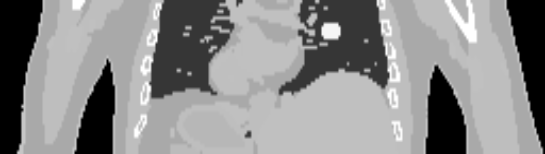
\includegraphics[width=1.0\linewidth]{figures/background_mu_map_example.png}
                    
                    \captionsetup{singlelinecheck=false, justification=raggedright}
                    \caption{Example of a simulated \gls{mu-map}, with no motion or noise, of the thorax with a spherical lesion in the lungs. Coronal view.} \label{fig:combined_pet_ct_mu_map_example}
                \end{figure}
                
                \begin{figure}
                    \centering
                    
                    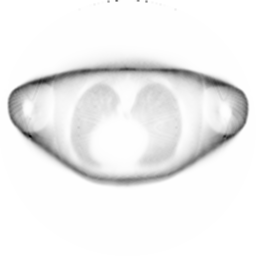
\includegraphics[width=1.0\linewidth]{figures/background_nac_example.png}
                    
                    \captionsetup{singlelinecheck=false, justification=raggedright}
                    \caption{Example of simulated \gls{NAC} \gls{TOF} data, with motion, with no noise randoms or scatters, of the thorax with a spherical lesion in the lungs. Transverse view.} \label{fig:combined_pet_ct_nac_tof_example}
                \end{figure}
                
                \begin{figure} %KT if you're bored (!),I'd put the NAC and AC figures next to eachother
                    \centering
                    
                    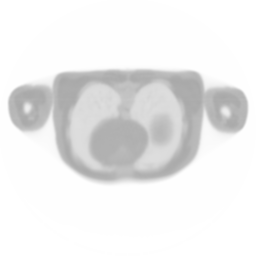
\includegraphics[width=1.0\linewidth]{figures/background_ac_example.png}
                    
                    \captionsetup{singlelinecheck=false, justification=raggedright}
                    \caption{Example of simulated \gls{AC} \gls{NTOF} data, with motion, with no noise, randoms or scatters, of the thorax with a spherical lesion in the lungs. Transverse view.} \label{fig:combined_pet_ct_ac_tof_example}
                \end{figure}
                
                As discussed previously in~\Fref{sec:attenuation} attenuation represents the loss of coincidences by photon interactions in matter. Attenuation is an issue in \gls{PET} as it causes the loss of signal and a degradation in image quality, this is the opposite for \gls{CT} where the modality itself relies on attenuation in order to differentiate anatomical structure, an example of a \gls{mu-map} can be seen in~\Fref{fig:combined_pet_ct_mu_map_example}. An example of some \gls{NAC} \gls{TOF} and \gls{AC} \gls{TOF} data can be seen in~\Fref{fig:combined_pet_ct_nac_tof_example} and~\Fref{fig:combined_pet_ct_ac_tof_example} respectively. %In order to find reasonable quantitative results the attenuation of the patient must be taken into account in \gls{PET}. Both \gls{PET} and \gls{CT} follow the Beer-Lambert law. %KT cut last sentence.not  relevant here %ACW done
                
                Methods to acquire \gls{mu-map}, for attenuation correction include; to take a transmission scan of a known point source rotated around the body of the  prior to the injection of the radiotracer. This allows for the estimation of the attenuation for each angle~\boxcite{TransmissionatnBib}. Another method involves the use of the known attenuation from the \gls{CT} scan.
                
                In order to apply the \gls{CT} based \gls{mu-map} to attenuation correction in \gls{PET} first it must undergo either bilinear or trilinear conversion to asses the attenuation coefficient factors, this is because of the relative energy difference of the two modalities~\boxcite{Carney2006}. As discussed above in~\Fref{sec:coincidence_processing} and~\Fref{sec:combined_pet_ct} \gls{PET} and \gls{CT} operate at two different energy levels of between between $425$ and $600$ \gls{KeV} and between $40$ and $140$ \gls{KeV} respectively~\boxcite{Bettinardi2011, CTattenuationenergyBib}.
                
                Issues with \gls{CT} based attenuation correction include: Firstly, as mentioned above in~\Fref{sec:combined_pet_ct}, \gls{CT} is acquired sequentially to \gls{PET} rather than simultaneously meaning that there can be mismatches in anatomy between the scans. Secondly, the propagation of any artefacts from the \gls{CT} volume into the \gls{PET} volume. Regardless of these issues \gls{CT} is currently considered to be the gold standard for \gls{mu-map} estimation for attenuation correction. Transmission scans are now very rarely used because of their sensitivity to user error, inclusion of an additional external source and their significant increase in scan time.
                %KT  Briefly mention MLAA here
                %ACW done
                
                Recently a method to jointly estimate both the activity and attenuation distributions has been proposed called \gls{MLAA}. This method takes one objective function which is defined in terms of the activity and attenuation and iterativley optimises for one of the distributions. This can be considered as at each step performing either emission or transmission tomography depending on the distribution being optimised for. Alternatively, it is also possible to optimise jointly for both distributions in one step~\boxcite{Fuin2017, Brusaferri2019}. A disadvantage of this solution is that without \gls{TOF} information it is possible for there to be significant cross talk artefacts between the activity and attenuation estimate~\boxcite{MLAASalomonBib, MLAADefriseBib}. Additionally, optimising for the attenuation distribution increases the complexity and computational effort required of a reconstruction algorithm.
                
    \longsection{Inverse Problems and Optimisation}{sec:inverse_problems_and_optimisation}
        
        
        \subsection{Inverse Problem Concepts} \label{sec:inverse_problem_concepts}
            An inverse problem is one where the original conditions of a system are attempted to be derived from the effects of the system. For instance, the data from a \gls{PET} scanner represents the observations of the distribution of the radiotracer in the patient, reconstruction is an attempt to find the distribution from these observations.
            
            Because it is not usually possible to directly invert to find the solution, because of the size of a given matrix for instance causing the computation time to find an inverse to be large, then the solution must be optimised for. In order to attempt to find the solution to an inverse problem there are two things which are required; first the forward operator is required which is the inverse of the inverse problem, which is being solved, or the forward problem, %KT true, but do you understand this? simplify by cutting
            second, ideally, a model of the noise present in the system is required. %KT what ``at least''. I'd say ``ideally'' %ACW done
        
        \subsection{Optimisation Concepts} \label{sec:optimisation_concepts}
            Optimisation means to find some values that best paramatrise some given function based on some criteria or objective. %KT I feel it needs something else ``based on some criteria'' or ``objective'' or ... %ACW done
            For instance, in reconstruction an optimisation could be to find the image that when it has the forward operator applied to it best matches the measured data. Another example of an optimisation would be to find the motion parameters that when applied to a given image most closely warp that image to match another image. Optimisation is also used in fields such as when training neural networks. Here the optimisation finds parameters for a model that maps one set of values to another, this will be discussed later in~\Fref{sec:machine_learning_for_pet}.
            
            In order to perform a basic optimisation there are four things which are required; an objective function to optimise  and a method to optimise some given values based on this function. Also, an initial estimate, which could be a volume the size of the output image filled with ones or zeros, and some method to cease execution, for instance stopping when the objective function reaches a certain value or the number of iterations exceeds a threshold, are also necessary. These will be discussed in the following sections in~\Fref{sec:objective_function} and~\Fref{sec:optimiser} respectively.
        
            \subsubsection{Objective Function} \label{sec:objective_function}
                Optimisation of some values requires a function that represents, for instance, the similarity of two measures or the likelihood of something given a measure. This function is required because in a sense the optimiser attempts to find some solution by either maximising or minimising the result of applying this function iteratively until either a maximum number of iterations or some other stopping criteria is reached.
                
                An example of an objective function would be \gls{MAE}. For a vector of some values, \gls{MAE} subtracts the estimated value from the true value, finds the absolute of this, sums together this value for all values in the vector and divides by the number of values in the vector. The absolute value is taken because the error should be the distance to the true value regardless of if the estimated value is greater or less than the true value. This method finds the mean error over all estimated values. If the estimated values approach the true values then the value of the \gls{MAE} will approach zero in a linear fashion. If \gls{MSE} is used then rather than taking the absolute of the error the square is taken instead, taking the square causes the error to increase quadratically as it becomes larger. %KT exponentially? no,quadratically %ACW done
                \gls{MAE} and \gls{MSE} are usually used in regression like problems where a line is fit though a data set.
                
                Another example of an objective function would be the likelihood. This function for any given sample of data returns the goodness of fit to a statistical model. %KT stricyl speaking, the likelihood will be related to minus the goodness of fit (higher likelihood, better fit, lower goodness-of-fit weirdly enough). maybe ignore
                The likelihood function describes a planes whose peak, if there is one distinct peak, %KT???
                represents the values which is %KT not maximise, it is the probability %ACW done
                the probability of drawing the sample obtained~\boxcite{Myung2003TutorialEstimation}. \gls{MLE} is often used in \gls{PET} image reconstruction.
                %KT could add 1 sentence that often an additional penalty is used to decrease sensitivity to noise
                
                Additionally to the objective function a regularisation term is often added, summed to the objective function value (after being scaled by an $\epsilon$), in order to decrease sensitivity to noise. An example of a regularisation term is \gls{RDP} used by \gls{GE} in Q.Clear~\boxcite{RossQ.Clear}.
                
            \subsubsection{Optimiser} \label{sec:optimiser}
                \begin{figure}
                    \centering
                        
                    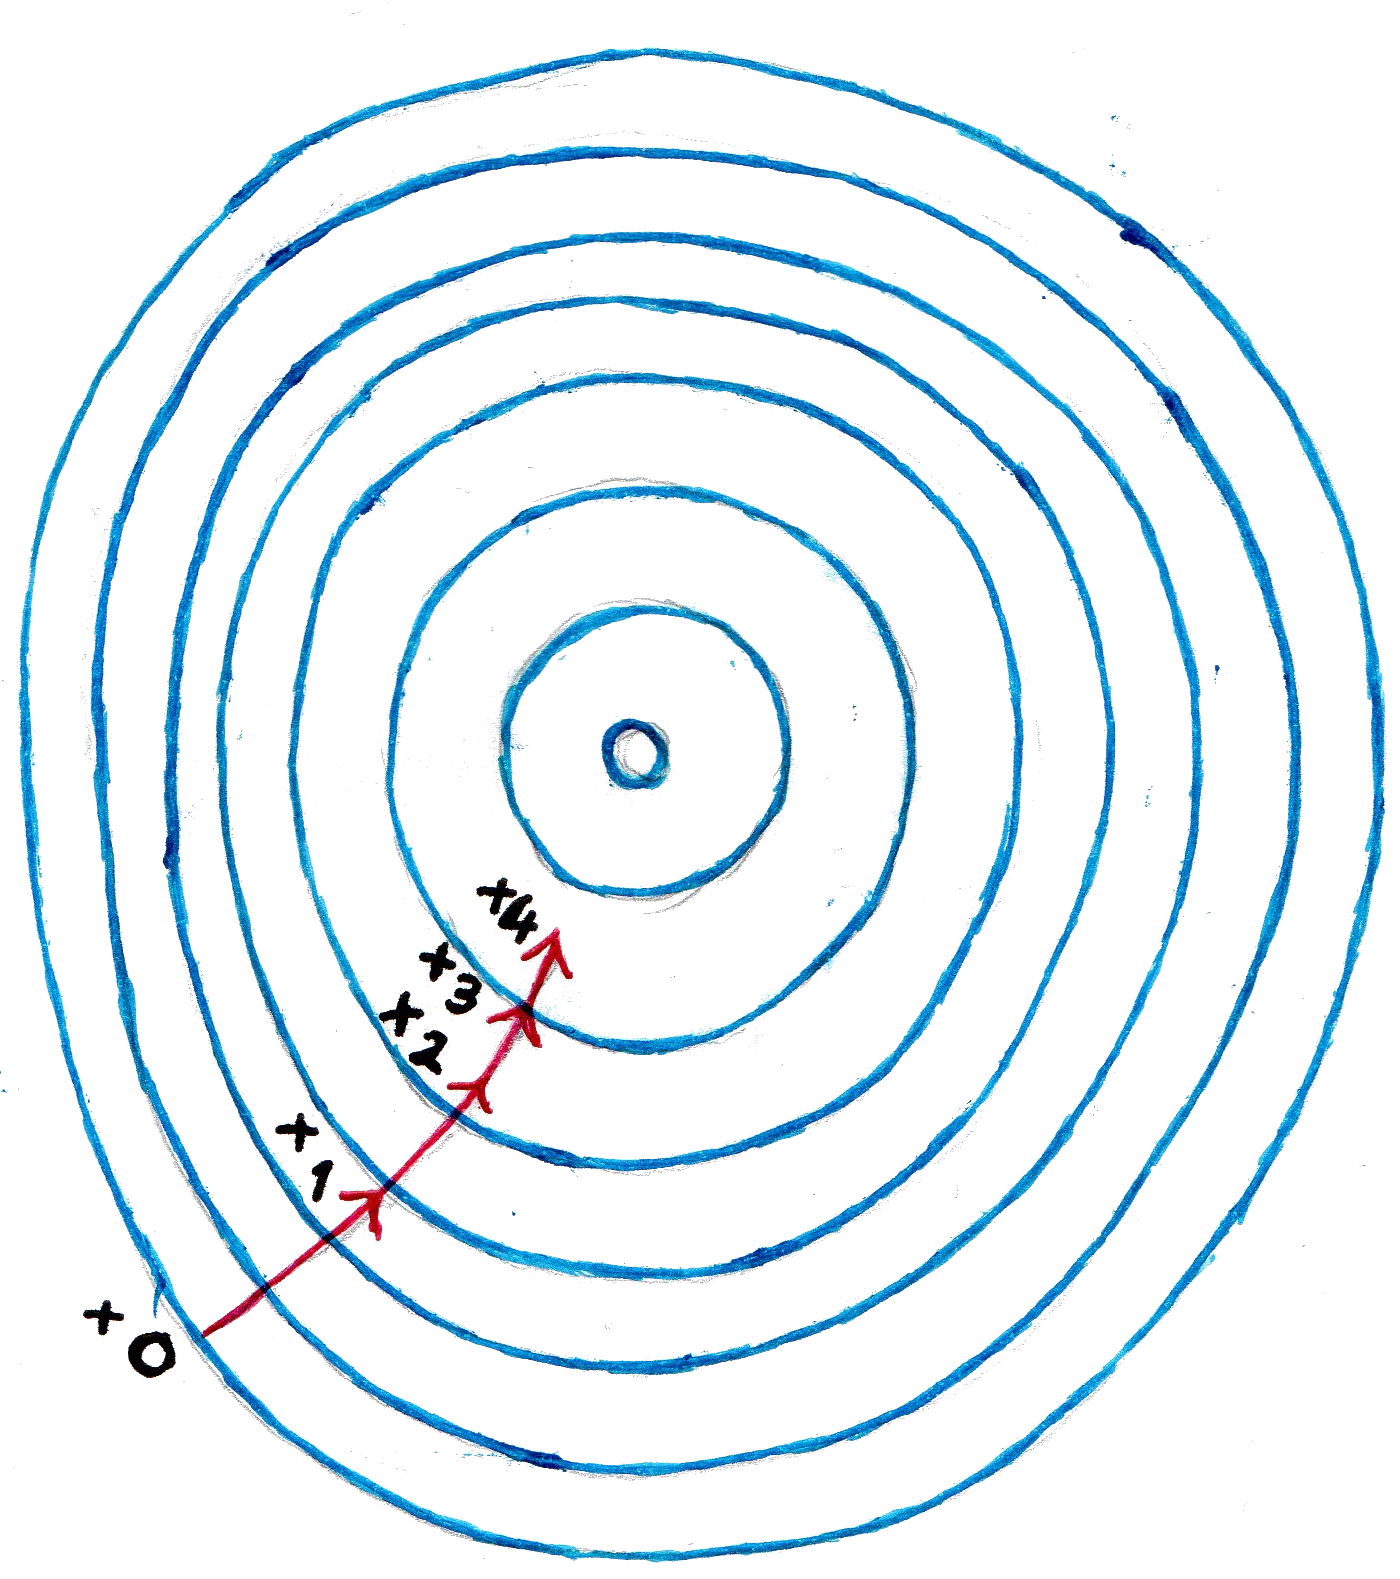
\includegraphics[width=1.0\linewidth]{figures/background_optimisation.png}
                        
                    \captionsetup{singlelinecheck=false, justification=raggedright}
                    \caption{Graphical representation of a \gls{2D} solution space and an optimiser stepping through this space. In the bottom left of this figure the initial estimate for some optimisation can be seen at $x$, the subsequent iterations $1$ through $4$ can then be seen taking this estimate closer to the centre of the contour plot. Here the contour plot could either be showing a maximisation or a minimisation depending on how it is visualised.} \label{fig:optimiser_optimisation}
                \end{figure}
                
                The optimiser takes an initial estimate of the values that are to be optimised and at least a function to either minimise or maximise the output of with the input of the estimate. This can be seen in~\Fref{fig:optimiser_optimisation}. The method by which the optimiser goes about updating the value of the estimate is what differentiates most optimisation algorithms.
                
                \gls{GD} is a commonly used optimisation algorithm. \gls{GD} finds the gradient of the objective function at the current estimate %KT?you mean ``at the current estimate'' %ACW done
                and takes steps, of a given size,  in the direction calculated from the gradient. %which most shrinks the value of the objective function. %KT ``most'' I think is only true for ``Steepest GD''. I'd cut the 2nd half of the sentence %ACW done
                The step size of \gls{GD} can be set to a fixed value or found using a line search which optimises the step size. Momentum can be used as an improvement of \gls{GD} where the current update direction is a linear combination, with a predefined weighting, of the current gradient and the previous update direction. %KT ok, although I wouldn't call it GD anymore. I'd therefore say ``Momentum can be used as an improvement of GD'' or so %ACW done
                %Momentum attempts to reduce the effect of local minimum solutions or non-convex solution spaces by reducing the likelihood of the current update causing the optimisation to jump back and forth between two close values. %KT I disagree with tis sentence. they just try to go faster. This methods have no clue about local minima etc %ACW done
                
                \gls{SGD} is an extension of \gls{GD} where the current update is calculated using the gradients of a randomly selected subset of the data, %KT of the data (not the estimate) %ACW done
                this is significantly more computationally efficient that \gls{GD} as it reduces the number of calculations needed for each update.
                
                \gls{CG} is another extension of \gls{GD}. Here the direction of subsequent updates are confined so that they are orthogonal to the previous update direction, this can decrease convergence time~\boxcite{Tustison2009}. %KT remove the ``can avoid the same issue''. CG also attempts to go to a local minimum %ACW done
            
    \longsection{PET Image Reconstruction}{sec:pet_image_reconstruction}
        The data output from a \gls{PET} scan are usually expressed in \gls{kBq/mL}, however for pseudo quantitative analysis the values are usually normalised to \gls{SUV} by dividing the activity by, for instance, the mass of the patient and the injected activity. %KT previous sentence belongs in image recon section, not where you discuss the measured data %ACW done
        
%        \subsection{Analytic Image Reconstruction} \label{sec:analytic_image_reconstruction}
            % mention briefely FBP ?
            %KT no! cut. I didn't read it
            %ACW done
%            \begin{figure}
%                \centering
                    
%                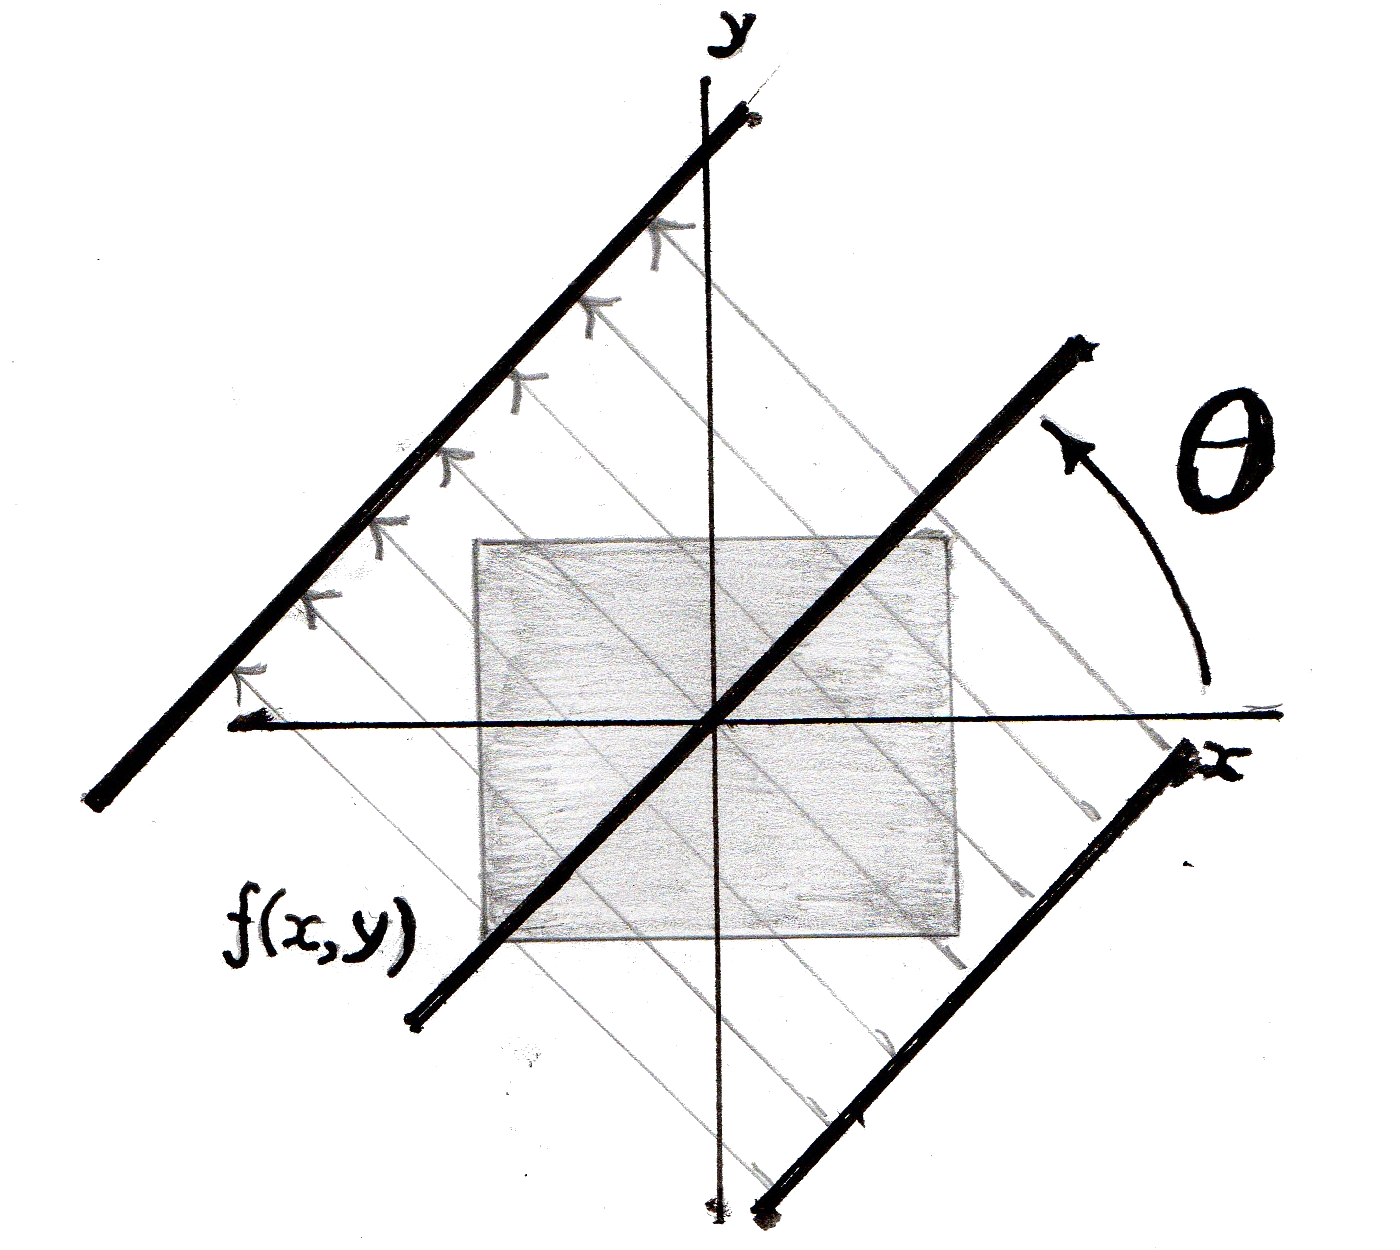
\includegraphics[width=1.0\linewidth]{figures/background_radon_transform.png}
                    
%                \captionsetup{singlelinecheck=false, justification=raggedright}
%                \caption{Graphical representation of the Radon transform for one angle $\theta$. The Radon transform computes projections of some data along specified directions. Here, this figure shows the computation of a set of line integrals for the function $f(x, y)$, usually from multiple sources of parallel beams. To form a full image the Radon transform rotates the source around the centre of the image. This figure specifically shows projections for a simple \gls{2D} image along horizontal and vertical components $x$ and $y$.} \label{fig:analytic_image_reconstruction_radon_transform}
%            \end{figure}
            
%            \begin{figure}
%                \centering
                
%                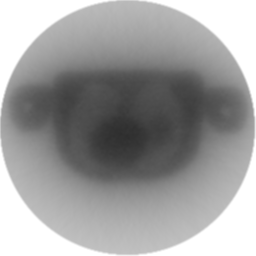
\includegraphics[width=1.0\linewidth]{figures/background_bp_example.png}
                
%                \captionsetup{singlelinecheck=false, justification=raggedright}
%                \caption{Example of a simulated \gls{AC} \gls{NTOF} \gls{BP} reconstruction, with motion and noise, with no randoms or scatters, of the thorax with a spherical lesion in the lungs. Transverse view.}
%                \label{fig:analytic_image_reconstruction_bp_example}
%            \end{figure}
            
%            \begin{figure}
%                \centering
                
%                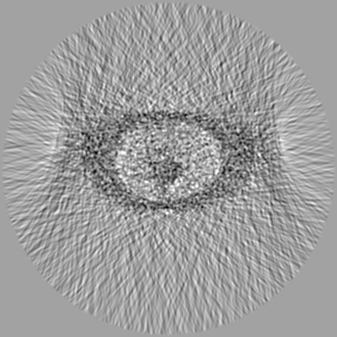
\includegraphics[width=1.0\linewidth]{figures/background_fbp_example.png}
                
%                \captionsetup{singlelinecheck=false, justification=raggedright}
%                \caption{Example of a simulated \gls{AC} \gls{NTOF} \gls{FBP} reconstruction, with motion and noise, with no randoms or scatters, of the thorax with a spherical lesion in the lungs. Transverse view.}
%                \label{fig:analytic_image_reconstruction_fbp_example}
%            \end{figure}
            
%            An analytic solution is one which offers a direct mathematical method through which one thing can be transformed to another. All analytical solutions can have a proof. An analytical solution for \gls{PET} reconstruction is \gls{BP}, in \gls{2D} \gls{BP} is the inverse Radon transform. This can be seen in~\Fref{fig:analytic_image_reconstruction_radon_transform}. To apply the inverse Radon transform to a \gls{2D} sinogram; first the rows of the sinogram, corresponding to $\SI{0}{^{\circ}}$ through $\SI{180}{^{\circ}}$, are taken individually and have the Fourier transform applied to them. Then the result of this is reshaped to polar coordinates so that each row is the diameter of a circle and a \gls{2D} Fourier transform is applied giving the final output image. The Fourier transform decomposes a function into its constituent frequencies. The \gls{2D} Fourier transform of a function computed along a line is equivalent to the 1D Fourier transform of the Radon transform along that line. This is called projection slice theorem. 
            
%            \gls{FBP} was proposed as a solution to some of the issues apparent in \gls{BP}, like the fact that \gls{BP} suffers from low frequency blurring. In \gls{FBP} a high pass ramp filter is applied to the sinogram before it is Fourier transformed, thus removing some low frequency information or blurring. A low pass ramp filter can also be applied at the same time which removes some high frequency information or noise, this then would be a band pass filter. An example of a \gls{BP} and \gls{FBP} reconstruction can be seen in~\Fref{fig:analytic_image_reconstruction_bp_example} and~\Fref{fig:analytic_image_reconstruction_fbp_example}. Because of its speed and good quantitative results \gls{FBP} was the gold standard of \gls{PET} image reconstruction, however because of the issues mentions above it has now almost entirely been replaced by iterative reconstruction methods. \gls{FBP} is now almost solely used in longitudinal studies which started before the use of iterative reconstruction methods became prevalent~\boxcite{FBPReviewBib, PETCTReviewBib}.
            
%            \gls{BP} and \gls{FBP} reconstruct a low quality image but are computationally fast. \gls{BP} will usually result in there being numerous streak like artefacts in the output image, the artefacts are exacerbated as noise increases. Artefacts can be caused because neither \gls{BP} nor \gls{FBP} account for the stochastic nature of the acquisition process, neither do they account for other factors such as positron range as discussed in~\Fref{sec:attenuation}.
            
            
        \subsection{Iterative Image Reconstruction} \label{sec:iterative_image_reconstruction}
            \begin{figure}
                \centering
                
                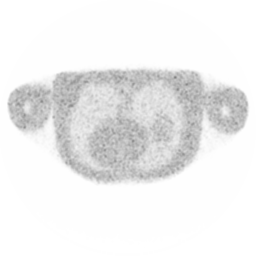
\includegraphics[width=1.0\linewidth]{figures/background_osem_example.png}
                
                \captionsetup{singlelinecheck=false, justification=raggedright}
                \caption{Example of a simulated \gls{AC} \gls{NTOF} \gls{OSEM} reconstruction, with motion and noise, with no randoms or scatters, of the thorax with a spherical lesion in the lungs. Transverse view.}
                \label{fig:iterative_image_reconstruction_osem_example}
            \end{figure}
            
            %As discussed above in~\Fref{sec:inverse_problems_and_optimisation} an inverse problem, which \gls{PET} reconstruction is, can be solved by an iterative optimisation problem. In order to implement an iterative optimisation problem a few criteria must first be met; a forward operator which takes an image and return the projections which would result from acquiring the image is required. As discussed above in~\Fref{sec:optimisation_concepts} an objective function to assess the accuracy of the fit and an optimisation algorithm to improve the fit are required. Also, an initial estimate, which could be a volume the size of the output image filled with ones or zeros, and some method to cease execution, for instance stopping when the objective function reaches a certain value or the number of iterations exceeds a threshold, are also necessary. %KT cut all this here as strong overlap with previous section. Move statement about initialestimate and stopping criteria there. %ACW done

            %KT cut some stuff if cutting analytic recons above
            An iterative method has the advantage that the model which is used can take into account the noise properties of the data and also the physical properties of the scanner itself. The noise associated with \gls{PET} is often assumed to be Poisson distributed. However, iterative methods have the disadvantage that because they are often significantly complex then they require substantial computational effort to execute which will increase computation time when compared to analytical reconstruction.
            
            %\gls{ML} is a commonly used objective function for iterative \gls{PET} reconstruction. This builds on the concepts, specifically \gls{MLE}, mentioned in~\Fref{sec:objective_function}. %KT cut previous sentence. no need to repeat all the time %ACW done
            When maximising the likelihood the natural logarithm of the likelihood, also known as the log-likelihood, is often taken for computational efficiency. \gls{ML} is often combined with the \gls{EM} algorithm for the optimisation of the model parameters and in this case is called \gls{MLEM}~\boxcite{MLEMBib,PETMLEMBib,PETMLEM2Bib}. The output from \gls{MLEM} commonly has a Gaussian blur applied in order to attempt to smooth noise~\boxcite{PETMLEMFiltBib}. Disadvantages associated with \gls{MLEM} include, that for noisy data iterating for too long can cause the output to accentuate the noise present in the data, one way to avoid this is to purposefully cease iterating early before the noise can take over the image~\boxcite{PETMLEMTerminationBib}. Another issue is that \gls{MLEM} is exceptionally slow even when compared to other iterative algorithms, as will be discussed below. %KT ``as mentioned earlier, as will be discussed below''. only the latter I guess %ACW done
            
            To combat the slow execution speed of \gls{MLEM} \gls{OSEM} was developed. In \gls{OSEM} \gls{LOR} or detector pairs of the scanner are binned into a number of subsets, in \gls{MLEM} there would be one subset and \gls{MLEM} would be applied to all \gls{LOR} or detector pairs simultaneously. However, in \gls{OSEM} the \gls{LOR} or detector pairs would be binned into at least two subsets and then \gls{MLEM} would be applied to each subset, in a specific order, sequentially~\boxcite{OrderedSubsetsHudsonBib, OrderedSubsetsHuttonBib}. Because the image is updated after each iteration of \gls{MLEM} on each subset of \gls{OSEM} then the execution speed of \gls{OSEM} is increased by the number of subsets used. However, %if more than two 
            subsets are used %KT even with 2 actually... %ACW done
            then  \gls{OSEM} will converge to a limit cycle around true convergence~\boxcite{Mettivier2011}. If a reasonable number of subsets are used then it has been found that \gls{OSEM} will accelerate \gls{MLEM} without affecting the accuracy of quantification too drastically~\boxcite{Morey2013}. An example of an \gls{OSEM} reconstructed image can be seen in~\Fref{fig:iterative_image_reconstruction_osem_example}.
            
    \longsection{Respiratory Motion in PET}{sec:respiratory_motion_in_pet}
        % general intro
        
        \subsection{Respiratory Motion Artefacts} \label{sec:respiratory_motion_artefacts}
            % have a look at https://www.sciencedirect.com/science/article/pii/S0001299808000214?via%3Dihub
            
            \begin{figure}
                \centering
                
                
\includegraphics[width=1.0\linewidth]{figures/background_motion_artefact_example.png}
                
                \captionsetup{singlelinecheck=false, justification=raggedright}
                \caption{Example of a simulated \gls{AC} \gls{NTOF} \gls{OSEM} reconstruction, with motion, with no noise, randoms or scatters, of the thorax with a spherical lesion in the lungs. Coronal view.}
                \label{fig:respiratory_motion_artefacts_motion_artefact}
            \end{figure}
            
            \begin{figure}
                \centering
                
                
\includegraphics[width=1.0\linewidth]{figures/background_single_mu-map_ac_example.png}
                
                \captionsetup{singlelinecheck=false, justification=raggedright}
                \caption{Example of a simulated single \gls{mu-map} \gls{AC} \gls{NTOF} \gls{OSEM} reconstruction, with motion, with no noise, randoms or scatters, of the thorax with a spherical lesion in the lungs. Coronal view.}
                \label{fig:respiratory_motion_artefacts_single_mu-map_ac}
            \end{figure}
            
            A single static bed position acquisition on a conventional \gls{PET} scanner takes approximately \SI{120}{\second}. This means that, because the patient is in respiratory motion throughout the acquisition, then the result of the scan will contain data from different respiratory states. During the different respiratory states the position and size of the lungs, diaphragm and any lesion will change. If the data is reconstructed all together then this will cause a blurring artefact especially prevalent around the anatomy that is moving the most, such as the diaphragm. %This would be expected as the data, in this case, represents as if the respiratory states had been summed together. %KT let's cut the previous sentence in an attempt to be less verbose :-) %ACW done
            An example of a \gls{PET} reconstruction with motion artefacts can be seen in~\Fref{fig:respiratory_motion_artefacts_motion_artefact}, notice the blurring above the diaphragm on the right side of the figure. Artefacts originating from the moving anatomy pose the largest challenge in imaging of the thorax~\boxcite{LungMotionArtefactBib, PETCTArtifactBib}.
            
            The artefacts caused by respiratory motion lead to issues clinically with cancer staging and follow up. This is because the size of the tumour is often over estimated and, because this causes the activity in the lesion to be spread out over more voxels, it also results in the activity being underestimated and to lesions potentially being missed due to reduced detectability~\boxcite{LungMotionJudgmentErrorsBib}. %KT and lesions potentially to be missed (i.e reduced detectability) %ACW done
            
            If attenuation is corrected for then the position of this \gls{mu-map} in relation to the position of the \gls{PET} data also poses an issue. Where the \gls{mu-map} does not match the position of the anatomy then it will cause either under or over correction for attenuation, this causes a type of artefact often referred to as a banana artefact for the shape of the shadow that it causes to appear above the diaphragm~\boxcite{LungMotionDiaphragmBaiBib}. An example of this can be seen in~\Fref{fig:respiratory_motion_artefacts_single_mu-map_ac}. Notice the black arc shaped artefact over the diaphragm and on the heart. The mismatch of the \gls{mu-map} and \gls{PET} data does not just cause this artefact but it can also change the expectation and thus the quantification of the reconstructed image will be affected. To combat intra-\gls{mu-map} motion the patient will often be asked to hold their breath, if they can, as the acquisition can only last between \SI{90}{\second} and \SI{150}{\second}~\boxcite{Nyflot}. An issue with this is, that often the breath hold \gls{CT} will be taken at full inspiration, if this \gls{mu-map} is then used to correct for attenuation in data that is in a respiratory phase other than full inspiration then a lot of this anatomy will have been moved into the \gls{FOV}. %KT this last sentence is incorrect. ``intra-mu-map'' motion can indeed by circumvented lrgely by breathold (as it's a CT). however, most people would do this at full inspiration, and then you get into serious trouble. %ACW done
            
        \subsection{Respiratory Motion Challenges in Combined PET/CT Imaging} \label{sec:respiratory_motion_challenges_in_combined_pet_ct_imaging}
            To overcome the issues mentioned in~\Fref{sec:respiratory_motion_artefacts}, specifically related to the mismatch between \gls{mu-map} and \gls{PET} data a number of solutions have been proposed:
            
            \begin{itemize}
                \item Firstly, a method which acquires \gls{PET} data over a prolonged acquisition and throws away any data where the patient is in a position other than the one that corresponds to the breath hold \gls{CT} \gls{mu-map}. For this all data which is not at either one of full expiration or full inspiration would be removed~\boxcite{Liu2010, Grootjans2014}. %KT I'd rather say that the CT is then at breathhold first. %ACW done
                Then the one breath hold \gls{CT} \gls{mu-map} would be warped to this data~\boxcite{LungMotionBreathHoldBib}. An advantage of this approach is that it not only would correct for the misalignment of \gls{mu-map} and \gls{PET} data but it would also eradicate any blurring associated with averaging over respiratory phases. A disadvantage is that,  either there would be substantially more noise in the reconstructed data (if the acquisition was the same length as a standard one) or the acquisition would need to take significantly longer, as so much data is being removed~\boxcite{Nehmeh2008a}. Additionally, dynamic scans would not be possible with this correction method. This is because the tracer kinetics could be shorter than one respiratory cycle and thus would be lost when those parts of the acquisition are removed.
                
                \item Secondly, a method similar to the first one has been proposed, this is where the \gls{PET} data is separated into individual images representing the separate respiratory phases. The one breath hold \gls{CT} \gls{mu-map} would then be warped in turn to each respiratory phase. This method provides the advantage over the first in that it uses all of the data from the \gls{PET} acquisition and provides a more robust reconstruction~\boxcite{4DPhaseMatchedReconBib}. A disadvantage is, that the reconstruction of each respiratory phase is likely to contain more noise than if all of the \gls{PET} data was reconstructed simultaneously. This is because the reconstruction algorithm is non-linear and summing reconstructed volumes is not the same as summing projection data, reconstructing and then summed again. %KT true, but you then first need to say that the images are summed again. %ACW done
                In addition, the higher levels of noise in the reconstructed data can pose a problem when attempting to warp the \gls{mu-map} to them.
                
                \item Finally, a method by where the reconstruction and motion parameters can be estimated simultaneously, directly from the \gls{PET} data, for one breath hold \gls{CT} \gls{mu-map} has been recently proposed~\boxcite{JacobsonFesslerMotionCorrectionBib, Rezaei2012, Bousse2016a}. Here, the \gls{PET} data is split into the respiratory phases, as above. Then it is iterated between a reconstruction step and a motion parameter estimation step where the same parameters are used to warp both the \gls{PET} data and the \gls{mu-map} for each respiratory position. Thus the \gls{mu-map} does not have to correspond to any one respiratory phase as each set of \gls{PET} data will be reconstructed at the position of the \gls{mu-map}. This method works especially well when \gls{TOF} data is available~\boxcite{Bousse2016b}. A disadvantage of this method is that it takes more computation than the above methods and that it has not been as extensively evaluated.
            \end{itemize}
    
    \longsection{Motion Correction for PET}{sec:motion_correction_for_pet}
        
    
        \subsection{Image Registration} \label{sec:image_registration}
            Image registration is an optimisation problem which attempts to take either an image or volume (called the static image or volume) to either a single or multiple images or volumes (called the dynamic images or volumes). The way that one image is taken to another image is through the use of a transformation. There are  different kinds of deformations including \gls{RD} and \gls{NRD} which will be discussed in the following sections. These deformations directly deform or warp the static image so that it best matches the dynamic image. %If there are multiple dynamic images then the optimisation will produce a transformation for each image.
            The images used for image registration do not necessarily need to be from the same modality and as such \gls{CT} data can be registered to \gls{PET} data and vice versa. A common use for image registration in medical imaging is to help in the process of \gls{MC}.
            
            As discussed in~\Fref{sec:optimisation_concepts} an optimisation requires an objective function. In the case of image registration the most common objective functions are \gls{MSE}, \gls{CC} and \gls{MI}. \gls{MSE} is discussed in~\Fref{sec:objective_function} but simply assumes that once the static image has been deformed to the dynamic then the images should be identical, thus \gls{MSE} is best used when the only difference between the two images is from motion, for instance. \gls{CC} and \gls{MI} are less reliant on the specific intensity values of an image and instead look for relationships between intensities, thus they are more suitable to registering between different modalities~\boxcite{Hill2001, Oliveira2014}.
            
            One difference between the optimisation for image registration and for image reconstruction is that the stochastic nature of the data is not usually taken into account in the model for image registration.
            
            \subsubsection{Rigid Deformation} \label{sec:rigid_deformation}
                \begin{figure}
                    \centering
                    
                    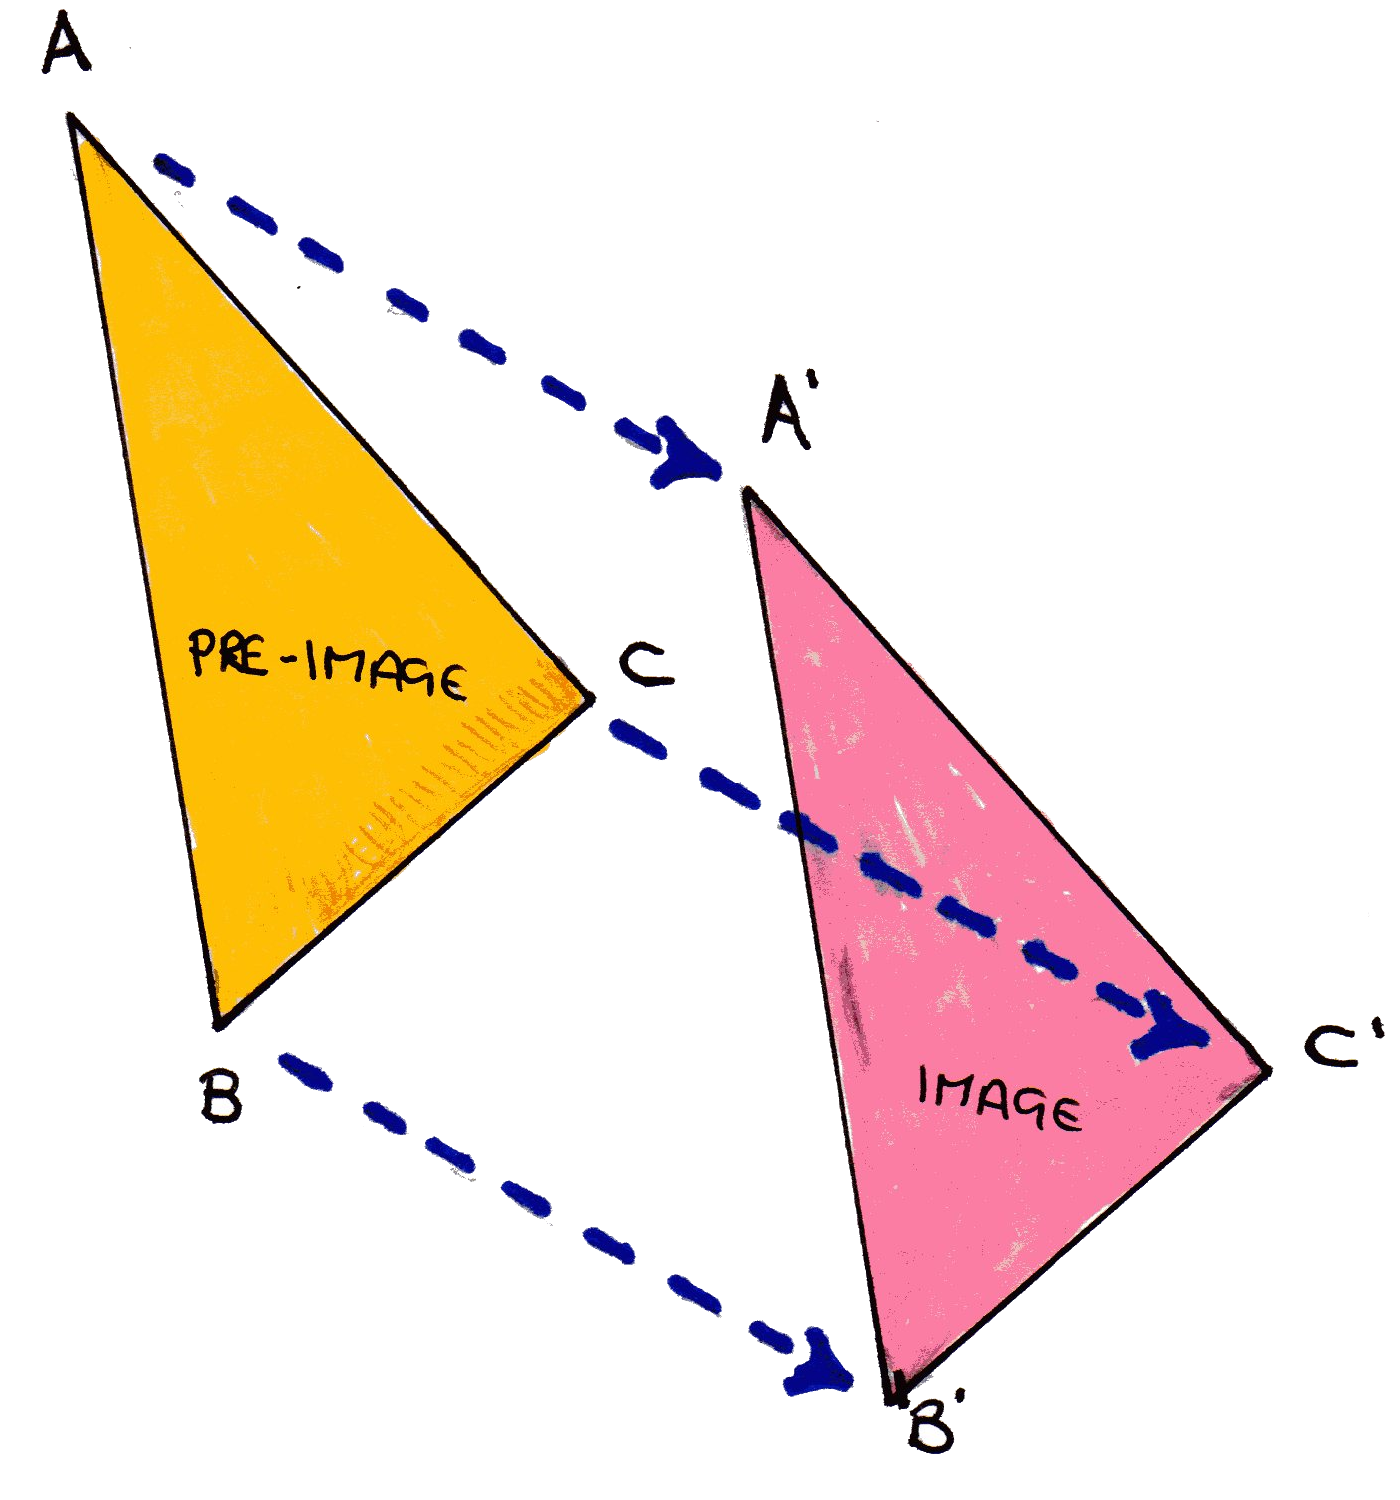
\includegraphics[width=1.0\linewidth]{figures/background_rd.png}
                    
                    \captionsetup{singlelinecheck=false, justification=raggedright}
                    \caption{Graphical representation of a \gls{RD}. On the left a triangle with vertices $A$, $B$ and $C$ can be seen, this triangle undergoes a \gls{RD} (a translation down and to the right) to a triangle, on the right, with vertices $A'$, $B'$ and $C'$.} \label{fig:rigid_transformations_rd}
                \end{figure}
                
                \begin{figure}
                    \centering
                    
                    \includegraphics[width=0.8\linewidth]{figures/background_ad.png}
                    
                    \captionsetup{singlelinecheck=false, justification=raggedright}
                    \caption{Graphical representation of an \gls{AD}. In the centre a cyan leaf can be seen which undergoes an \gls{AD} (a translation down and to the left, a rotation anticlockwise and a scale down) to a red leaf, on the left. The cyan leaf also undergoes an \gls{AD} (a translation down and to the right, a rotation clockwise, a scale down and a skew) to a blue lead, on the right.} \label{fig:rigid_transformations_ad}
                \end{figure}
                
                A \gls{RD} would be a rotation or a translation of the entire contents of an image where the same rotation or translation is applied at every point. A \gls{RD} is one where the euclidean distance between every pair of points in the image is consistent before and after the deformation is applied, this can be seen in~\Fref{fig:rigid_transformations_rd}. \gls{RD} is a subset of a type of deformation called an \gls{AD}. A \gls{3D} \gls{RD} has six degrees of freedom, rotation and translation in every axis whereas a \gls{3D} \gls{AD} has $12$ degrees of freedom, rotation, translation, scaling and sheering in every axis. a \gls{AD} does not guarantee that the euclidean distance between pairs of points are maintained, this can be seen in~\Fref{fig:rigid_transformations_ad}.
                
                \gls{RD} are often used in medical imaging where the anatomy which is being registered is not expected to undergo individual internal motion, for instance \gls{RD} is often used in the registration of patient head motion. \gls{AD} are not often used in medical imaging as anatomy does not usually deform specifically in ways that \gls{RD} cannot capture but \gls{AD} can, although an initial \gls{AD} can be used as an initial starting point for more complex \gls{NRD}.
                
                The output from a \gls{RD} or \gls{AD} is usually the values from the six or $12$ value transformation matrix respectively and as such they do not take up much computational memory or storage.
                
            \subsubsection{Non-Rigid Deformation} \label{sec:non_rigid_deformation}
                \begin{figure}
                    \centering
                    
                    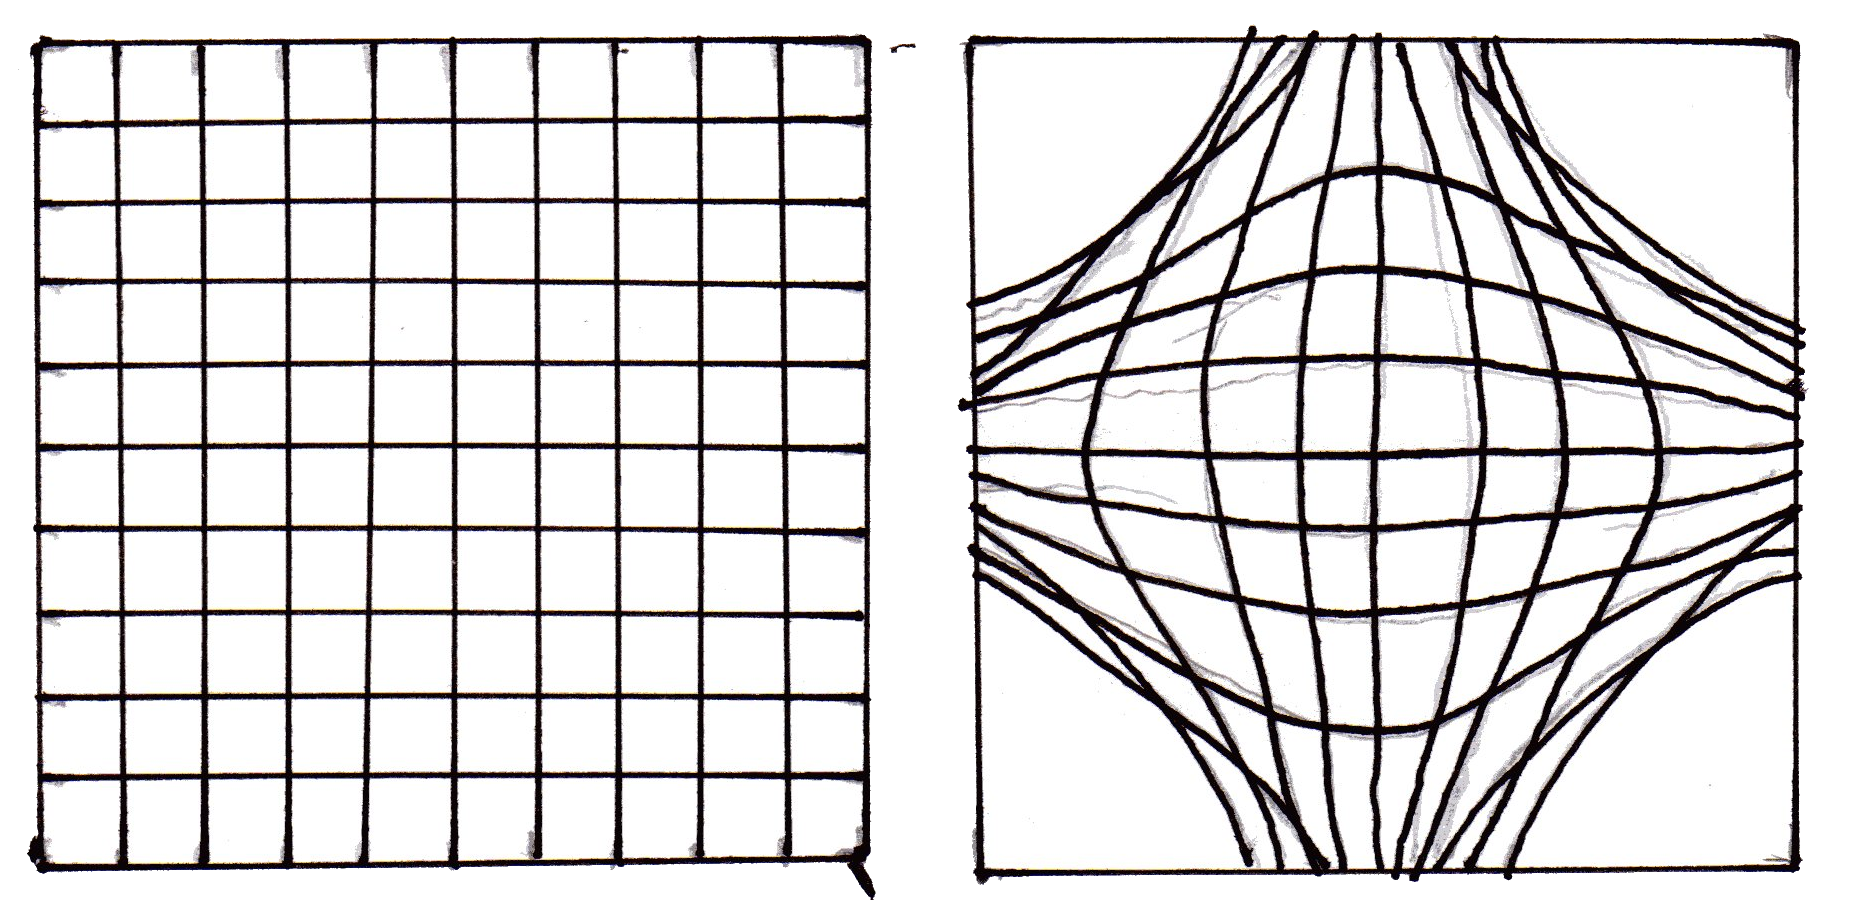
\includegraphics[width=1.0\linewidth]{figures/background_nrd.png}
                    
                    \captionsetup{singlelinecheck=false, justification=raggedright}
                    \caption{Graphical representation of a \gls{NRD}. On the left a grid can be seen, this grid undergoes a \gls{NRD} to the grid on the right.} \label{fig:non_rigid_deformation_nrd}
                \end{figure}
                
                A \gls{NRD} is one where the euclidean distance between pairs of points is not maintained, this can be seen in~\Fref{fig:non_rigid_deformation_nrd}. Notice that the euclidean distance between where the lines of the grids intersects changes between the grid on the left and the grid on the right. %For example the motion of a fluid is a \gls{NRD} as pairs of points can move past each other by different amounts.
                \gls{NRD} is commonly seen in medical imaging in respiratory motion as the diaphragm and lungs experience sliding motion and displace different parts of the patient's anatomy by different amounts. A \gls{NRD} is often parameterised as a \gls{DVF} where, in the simplest case, the warp is represented by a volume the same size, with the same number of elements, as the data where each element in the warp is a vector that either points from the position of the static image to the new position in the dynamic image or vice versa. However, for reasons of computational efficiency and to regularise the image registration optimisation, somewhat, usually the size of the warp volume is smaller than the data volume. Here \gls{CP} on a \gls{CPG} are interpolated using, for instance, linear or b-spline interpolation to find the vector to be applied to each point~\boxcite{Bardinet1996, Rueckert1999, Mattes2003, JacobsonFesslerMotionCorrectionBib}.
                
                Regularisation terms are often employed for \gls{NRD} image registration as otherwise with a high enough resolution \gls{CPG} it's possible for the optimisation to fit the noise present in the data rather than fitting the motion, as discussed in~\Fref{sec:optimisation_concepts}. One common form of traditional regularisation term used is the smoothness penalty from \gls{TPS}. Here, the term is calculated as the integral of the square of the second derivative of the \gls{DVF}, this term is multiplied by some value $\epsilon$ representing the weighting of this penalty term and then summed to the current value of the objective function. This regularisation term attempts to enforce that adjacent \gls{CP} should not rapidly change as this type of motion is unlikely physically~\boxcite{Duchon1977SplinesSpaces}.
        
        \subsection{Respiratory Gating} \label{sec:respiratory_gating}
            % brief intro
            
            \begin{figure}
                \centering
                    
                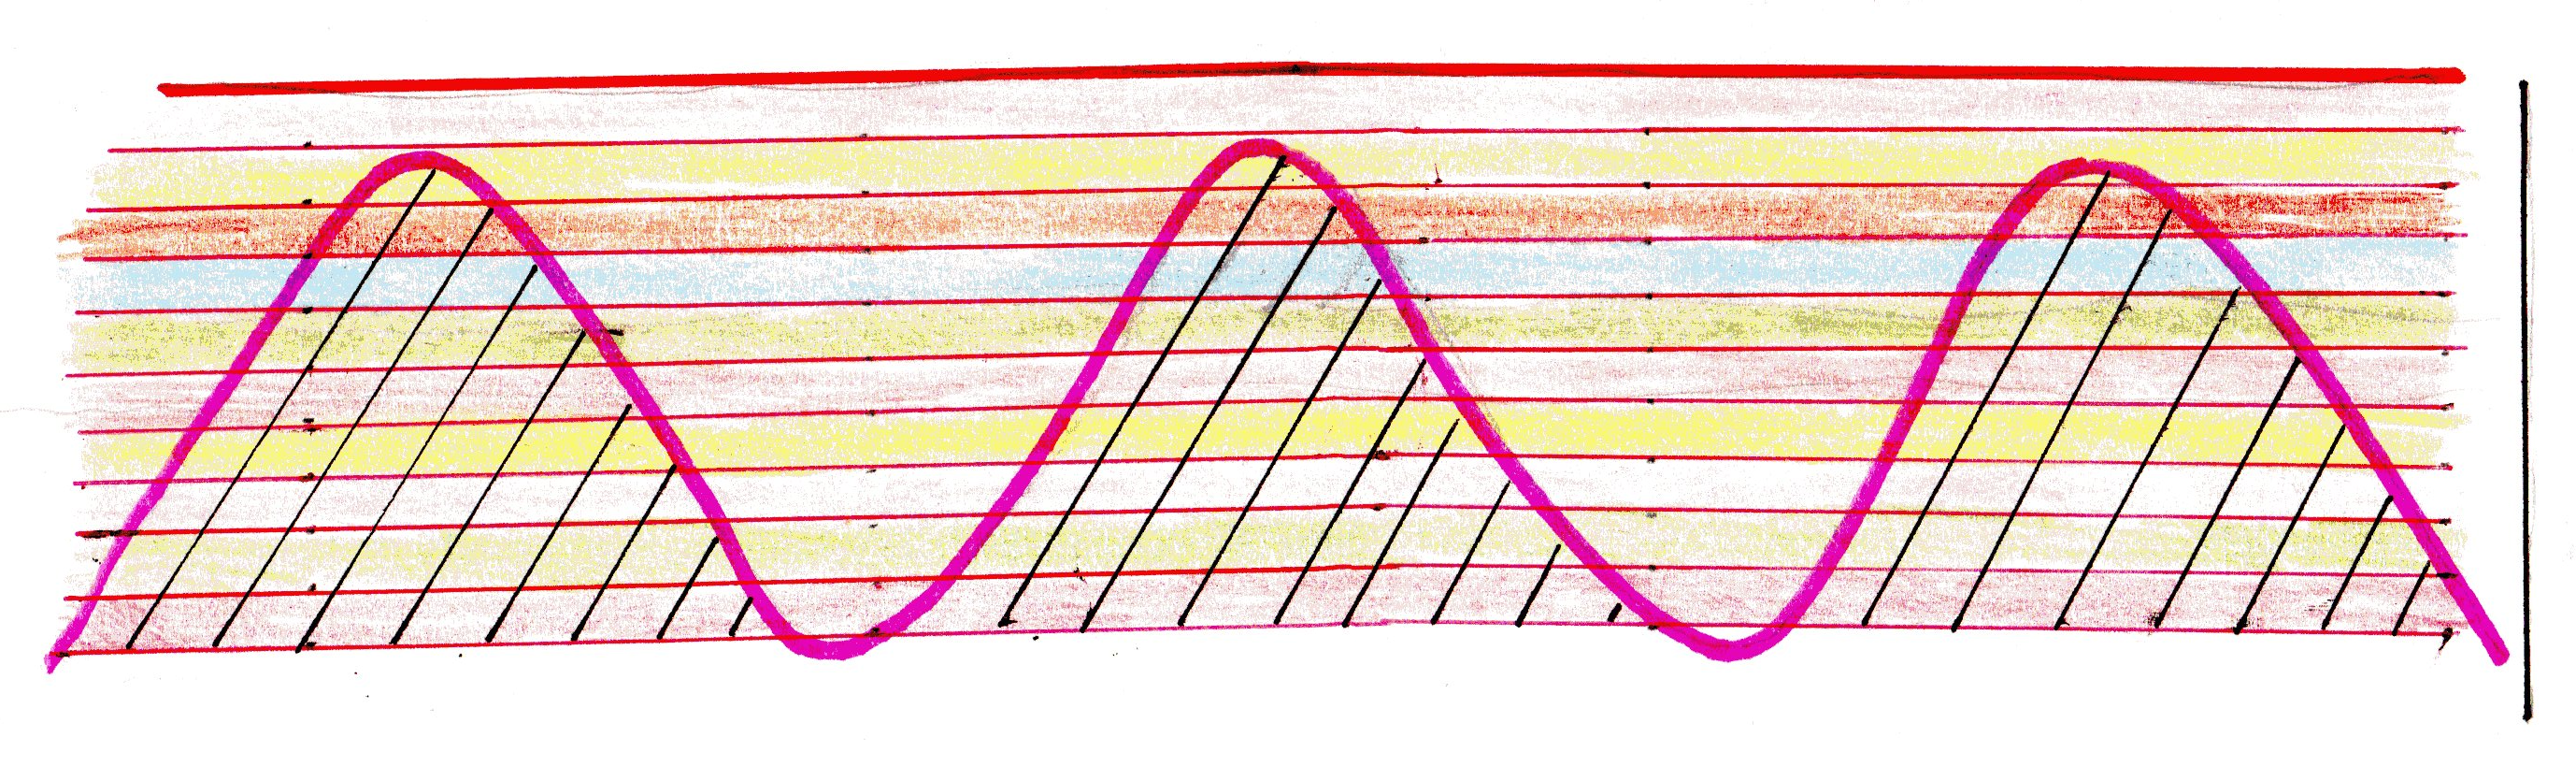
\includegraphics[width=1.0\linewidth]{figures/background_amplitude_gating.png}
                    
                \captionsetup{singlelinecheck=false, justification=raggedright}
                \caption{Graphical representation of amplitude gating. Here the red pseudo sinusoidal signal represents the \gls{SS} and the horizontal lines, colour coded differently, represent the, amplitude, gates that the data upon the \gls{SS} would be binned into.} \label{fig:respiratory_gating_ampliude_gating}
            \end{figure}
            
            \begin{figure}
                \centering
                    
                \includegraphics[width=1.0\linewidth]{figures/background_full_phase_gating.png}
                    
                \captionsetup{singlelinecheck=false, justification=raggedright}
                \caption{Graphical representation of phase gating. Here the red pseudo sinusoidal signal represents the \gls{SS} and the vertical lines, colour coded differently, represent the, phase, gates that the data upon the \gls{SS} would be binned into.} \label{fig:respiratory_gating_full_phase_gating}
            \end{figure}
            
            The method of respiratory gating was briefly touched on previously in~\Fref{sec:respiratory_motion_challenges_in_combined_pet_ct_imaging}. Here the process of specifically how respiratory gating works will be addressed. In order to either gate so that only counts in a certain window are accepted or to gate the acquired data into the respiratory phases, first a \gls{SS} which reflects the respiratory state of the patient, over time, must be acquired. This \gls{SS} can either directly reflect the amplitude of the patients breathing or can be a percentage of the phase through which the patient is in the respiratory cycle. These two types of \gls{SS} directly influence the type of gating that will be performed, these two types are:
            
            \begin{itemize}
                \item Firstly, amplitude gating takes the maximum and minimum value of the \gls{SS} and splits the values between them into a number of gates, this can be seen in~\Fref{fig:respiratory_gating_ampliude_gating}. The gates can be chosen so that they are either equally spaced apart or so that each gate has a similar number of elements binned into them. The acquisition data is binned by taking its relevant \gls{SS} value and summing it in into the gate which the value falls between.
                
                \item Secondly, phase gating works exactly the same way as amplitude gating but rather than splitting the data up along the \gls{SS} it can be conceptualised as splitting the data up temporally by the phase of the respiratory cycle, this can be seen in~\Fref{fig:respiratory_gating_full_phase_gating}.
            \end{itemize}
            
            Both types of respiratory gating can be augmented by incorporating other signals. For instance, amplitude gating can bin data into gates for both the inspiration and expiration parts of the respiratory cycle by also gating over the gradient of the \gls{SS}~\boxcite{Low2005}.
        
        \subsection{Respiratory Signal Detection} \label{sec:respiratory_signal_detection}
            As mentioned in~\Fref{sec:respiratory_gating} it is necessary to acquire information about the position in the respiratory cycle that the patient is in for respiratory gating but also for \gls{MM}. There are two types of methods through which \gls{SS} can be obtained. These are from external mechanical or electrical devices, which somehow physically measure the patient, or through \gls{DD} algorithms which attempt to extract the \gls{SS} from the data of the acquisition itself.
            
            \subsubsection{External Devices} \label{sec:external_devices}
                \begin{figure}
                    \centering
                        
                    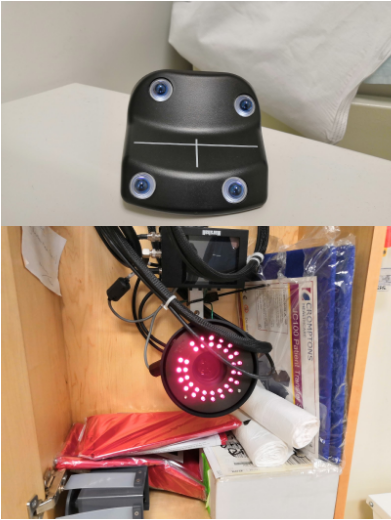
\includegraphics[width=1.0\linewidth]{figures/background_rpm.png}
                        
                    \captionsetup{singlelinecheck=false, justification=raggedright}
                    \caption{Photograph of \gls{RPM}. On the bottom is the infrared camera and infrared \gls{LED} used to locate and track an infrared reflecting marker. On the top is the infrared reflecting marker which is placed onto the chest or stomach of the patient in order to track the respiratory amplitude of the patient. Four reflective points are used to track the marker in \gls{3D} plus a point for redundancy.} \label{fig:external_devices_rpm}
                \end{figure}
                
                \begin{figure}
                    \centering
                    
                    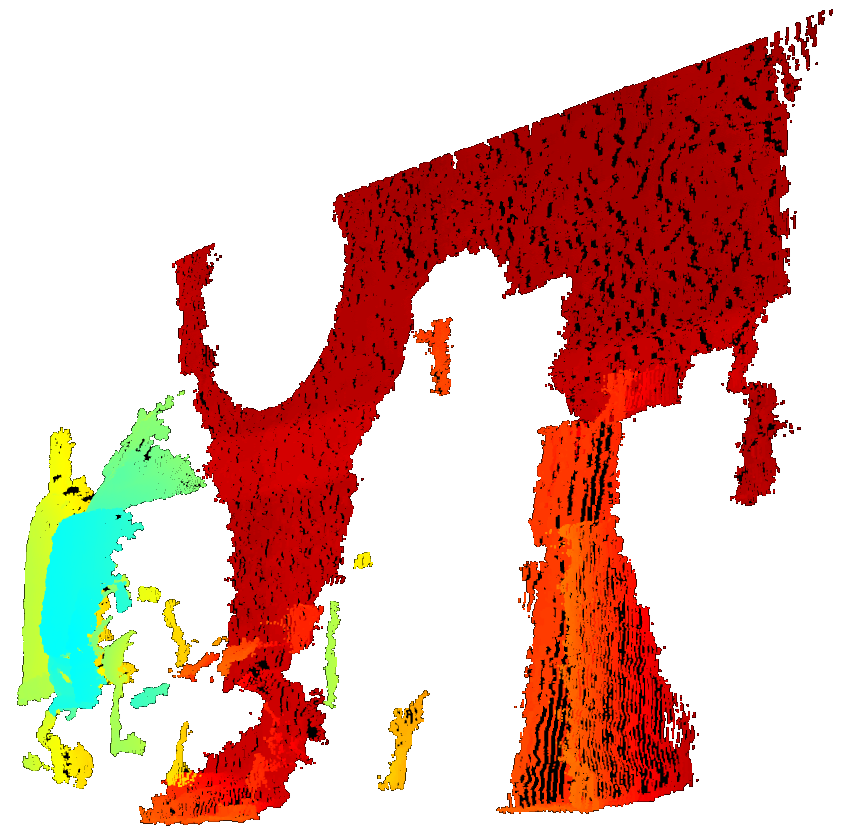
\includegraphics[width=1.0\linewidth]{figures/background_3dpc_example.png}
                    
                    \captionsetup{singlelinecheck=false, justification=raggedright}
                    \caption{Example of a \gls{3DPC} acquired on a Microsoft Kinect camera.}
                    \label{fig:external_devices_3dpc_example}
                \end{figure}
                
                There are numerous external device methods used to track a \gls{SS}. As an example four devices are:
                
                \begin{itemize}
                    \item Firstly, the oldest method of \gls{SS} tracking presented here is the use of a spirometer. A spirometer is a device with a tube which is inserted into the mouth of the patient through which they breath. The spirometer measures the volume of air and the velocity with which the patient inhales or exhales this air~\boxcite{Guivarch2004SynchronizationPlethysmography}. Some disadvantages of this method include; %that it is difficult to temporally synchronise the acquisition of the \gls{PET} data with the data from the spirometer. Additionally,
                    because spirometers are not designed for highly accurate measurement, over time, they are susceptible to value drift where the mean position of the respiratory cycle is not consistent between cycles~\boxcite{Hoisak2004}.
                    
                    \item Secondly, a method borrowed from radiotherapy for \gls{SS} tracking is through the use of the Varian \gls{RPM}. The \gls{RPM} was designed to be used in radiotherapy to turn on and off the beam of a linear accelerator. This would work by using the infrared camera of the \gls{RPM} to track a reflective marker placed on the stomach or chest of the patient tracking the displacement of the chest wall over time. This can be seen in~\Fref{fig:external_devices_rpm}. The Anzai AZ-733V system attempts to acquire the displacement of the abdomen, similarly to the \gls{RPM}, but uses a pressure belt wrapped around the patient. In radiotherapy, as the patient moves the target of the linear accelerator would also move so its beam is only turned on when the target is within range. In \gls{PET} the \gls{RPM} has been modified to output a clock tick to the computer acquiring the \gls{PET} data, this computer will %then synchronise with the \gls{RPM} clock and 
                    record timing information into the \gls{PET} data in order to align the \gls{RPM} \gls{SS} post acquisition. This method has the advantage over the spirometer in that it is significantly less susceptible to drift. However, the use of the \gls{RPM} increases scan time and as such receives push back from radiographers.
                    
                    \item Thirdly, optical cameras or laser based cameras, such as the Microsoft Kinect, can be used to determine a segmentation or, through the \gls{TOF} of the lasers, a \gls{3DPC} of the patient, at each time point. An example of a \gls{3DPC} acquired on a Microsoft Kinect camera can be seen in~\Fref{fig:external_devices_3dpc_example}. A \gls{3DPC} is a collection of coordinates measured as points on the surface of the object being scanned at some displacement. These segmentations or \gls{3DPC} can then be tracked by finding the difference in this segmentation or \gls{3DPC} over time~\boxcite{Miranda2017MarkerlessAnimals}. Advantage of this solution include;  it doesn't include the use of a reflective marker on the patient and as such should reduce scan time. Additionally, an optical or laser based camera can track motion over a larger \gls{FOV} than the \gls{RPM}. For instance, an optical or laser based camera could conceivably simultaneously track both respiratory and head motion, producing a \gls{DVF} directly for use in \gls{MC} or a \gls{SS}. A disadvantage is that it is much more difficult to spatially and temporally align the acquisition of both a \gls{PET} scanner and a stand alone optical or laser based camera~\boxcite{Noonan2012AccurateKinect, Noonan2015RepurposingPET, Whitehead2018MotionPET/CT}.
                    
                    \item Finally, on \gls{MR} scanners, there is the \gls{MR} navigator. During an \gls{MR} protocol there are times when the \gls{MR}, if told to do so, can measure specific small areas of the patient anatomy. An \gls{MR} navigator can be used to measure a pencil shaped \gls{1D} area, for instance, the position of the diaphragm or the chest wall of the patient. An advantage of this is that multiple navigators can be places to track more than one \gls{SS}. This works by looking for edges along the \gls{1D} pencil and assuming that the edge reflects the current position of the diaphragm or chest wall. An advantage of this is that it does not require any other additional equipment other than the \gls{MR} scanner and does not significantly affect scan time. A disadvantage is that it requires a \gls{MR} scanner which is not available in a \gls{PET}/\gls{CT}.
                \end{itemize}
                
            \subsubsection{Data Driven} \label{sec:data_driven}
                \begin{figure}
                    \centering
                        
                    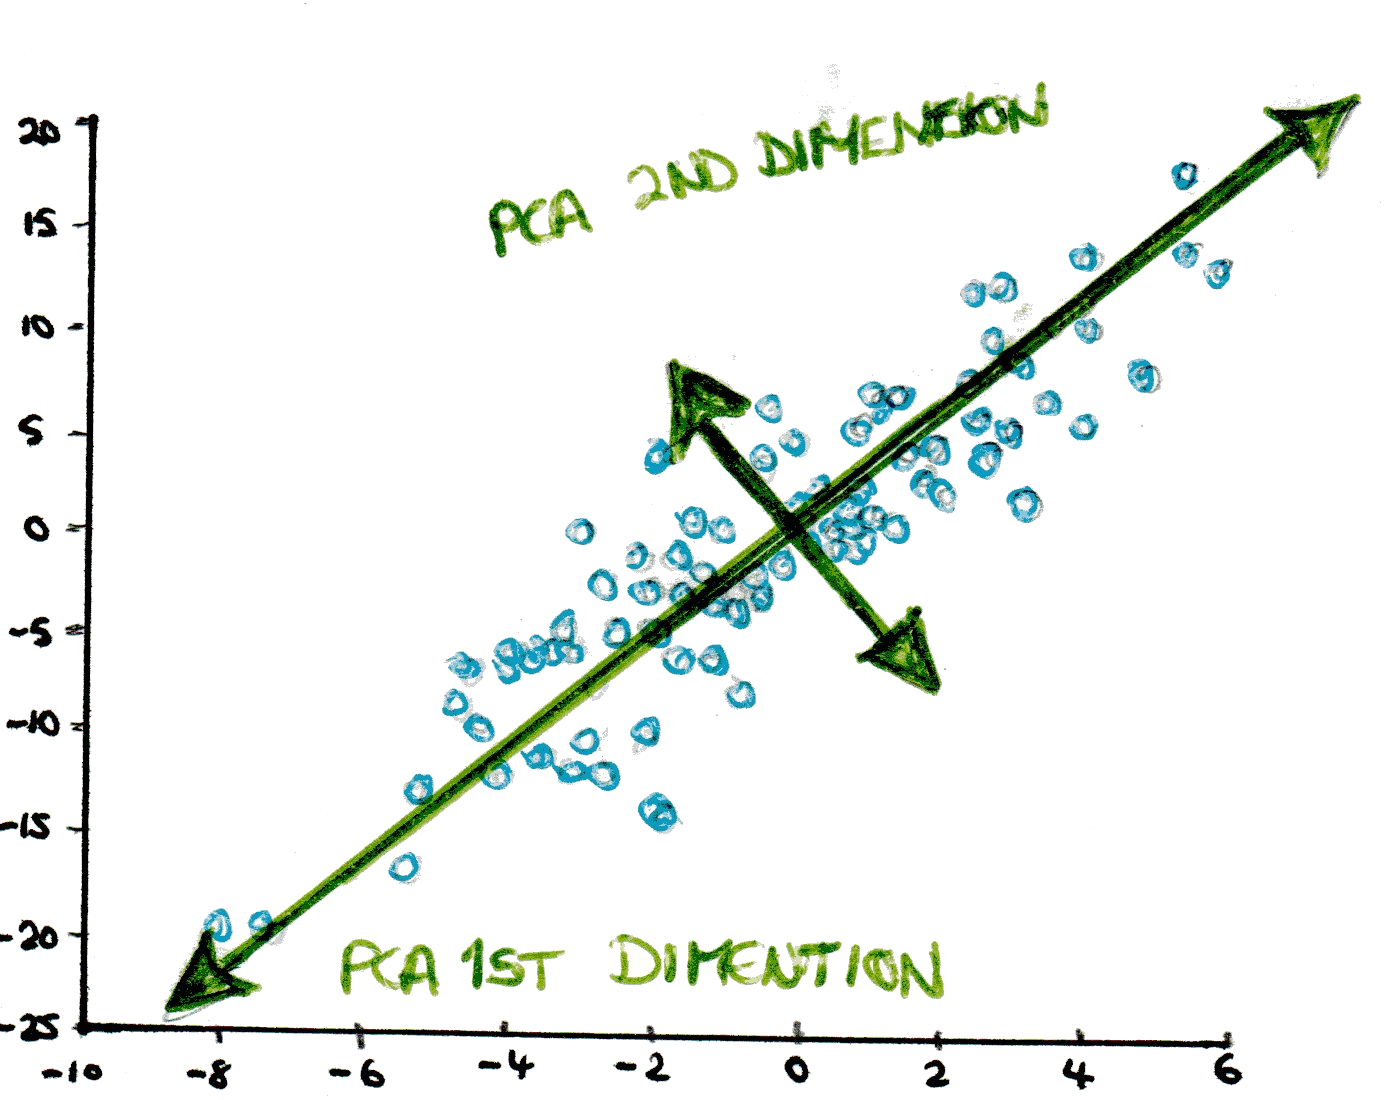
\includegraphics[width=1.0\linewidth]{figures/background_pca.png}
                        
                    \captionsetup{singlelinecheck=false, justification=raggedright}
                    \caption{Graphical representation of \gls{PCA} applied to \gls{2D} data. In the centre the \gls{2D} data points on which \gls{PCA} has been applied can be seen. From bottom left to top right the first eigenvector can be seen with most variance, from top left to bottom right the second eigenvector can be seen with less variance.} \label{fig:data_driven_pca}
                \end{figure}
                
                \begin{figure}
                    \centering
                        
                    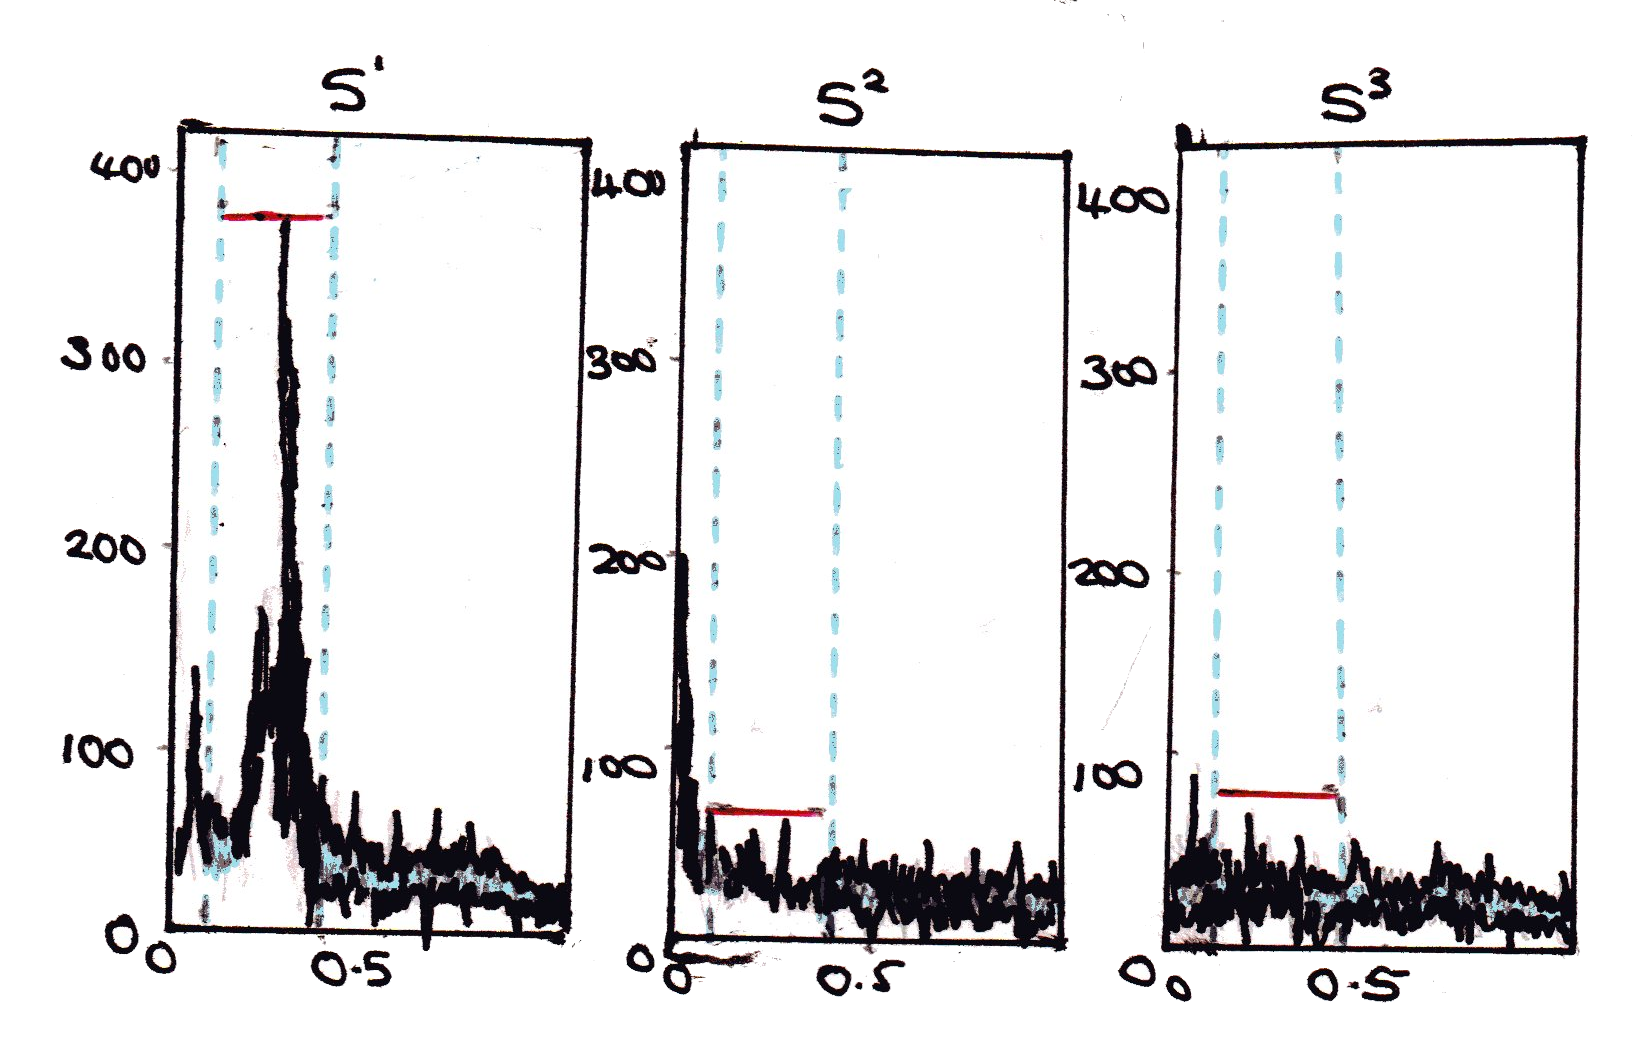
\includegraphics[width=1.0\linewidth]{figures/background_pca_window.png}
                        
                    \captionsetup{singlelinecheck=false, justification=raggedright}
                    \caption{Graphical representation of the frequency spectrum for three \gls{PC}. On the right a frequency spectrum of one \gls{PC} with a frequency window between \SI{0.1}{\hertz} and \SI{0.4}{\hertz} and a low value peak in this window can be seen. In the centre another example of what can be seen on the left can be seen. On the left another frequency spectrum with a frequency window can be seen, however, here the peak in the frequency window is significantly higher than in the other two examples.} \label{fig:data_driven_pca_windoe}
                \end{figure}
                
                There are numerous \gls{DD} methods used to extract a \gls{SS} directly from \gls{PET} data. Some methods require that the \gls{PET} data be reconstructed and then markers, possibly inserted into the patient, are tracked over time. Methods requiring reconstruction are mostly inferior to methods which work with \gls{PET} acquisition data. This is because requiring that reconstruction be performed takes significant time and the \gls{SS}, itself, is usually required for most \gls{MC} so the initial reconstructions will be poor. Here, of the methods using \gls{PET} acquisition data, only \gls{PCA} will be discussed as it has been proven that most static \gls{DD} \gls{SS} extraction methods perform similarly~\boxcite{2013ComparisonData}. Additionally, \gls{PCA} is the method of choice on \gls{GE} scanners.
                
                \gls{PCA} is a dimensionality reduction technique appied to data, closely related to \gls{SVD}, which attempts to find a transformation that maps the data to a lower dimensional space where the underlying structure of the data can be better determined~\boxcite{Pearson1901LIII.Space}. \gls{PCA} produces, for the data, a series of eigenvectors and eigenvalues where the eigenvectors are the orthogonal vectors of descending variance through the data and the eigenvalues are the scale of these eigenvectors, this can be seen in~\Fref{fig:data_driven_pca}. Thus the first eigenvector from \gls{PCA} will represent the vector of greatest variance through the data, in thoracic \gls{PET} this will usually be caused by the respiratory motion of the patient.
                
                When applied specifically to \gls{PET} acquisition data \gls{PCA} is often used on either sinograms or unlisted listmode data, the resultant sinograms are usually spatially downsampled. This is for a number of reasons including; the noise present in the full data would obscure the motion. Additionally, the large size of the \gls{PET} sinograms provides issues when it comes to storing the number needed in memory and the computational expense needed to apply \gls{PCA}, generally all of the data which the method will be applied to must be in memory simultaneously. Furthermore, the non-downsampled sinograms contain more than enough information for \gls{PCA} to be able to extract the relevant variation, thus if all the data was used then time would be wasted processing all of the data. Generally when used to extract respiratory variation the time frame of the \gls{PET} sinograms is chosen as \SI{0.5}{\second} so as to attempt to mitigate cardiac motion by allowing most of it to be averaged in each frame while still allowing for respiratory motion between frames~\boxcite{Bertolli2018Data-DrivenTomography}.
                
                The \gls{PC} which contains the variation present in the data caused by respiratory motion must be identified. One method to do this is as follows; first, the frequency spectrum of each \gls{PC} is required, this shows at what frequency variation occurs along each \gls{PC}. Then a frequency window is determined, this is usually between \SI{0.1}{\hertz} and \SI{0.4}{\hertz} so as to coincide with the approximate frequency of respiration. The max value or peak in the frequency spectrum is then found for each \gls{PC} in this window. The \gls{PC} which has the largest peak in the window is determined as being the one best representing variance caused by respiratory motion, this can be seen in~\Fref{fig:data_driven_pca_windoe}~\boxcite{Thielemans2011}.
                
                Evaluations have been performed on the \gls{PCA} method to both \gls{RPM} and \gls{MR} navigator based \gls{SS}. When compared to both external methods \gls{PCA} was shown to be relatively robust, specifically showing a correlation of $0.89$ for nine patients when compared to the \gls{MR} navigator based \gls{SS}~\boxcite{2013ComparisonData, Manber2015PracticalPET/MR.}.
                
                An advantage of the \gls{PCA} \gls{SS} extraction method over external device \gls{SS} tracking is that the \gls{PCA} method allows for \gls{SS} extraction at any point during the scan, once \gls{PET} acquisition data has been acquires of the thorax, even post scan. \gls{PCA} can be applied automatically without the intervention of a clinician thus not affecting acquisition time or inserting any additional steps into clinical practise. \gls{PCA} is also usually more comfortable for the patient as it does not involve any effort from them, in either being strapped into or otherwise having to interact with a device. This is all the while, as discussed above, providing accurate results when compared to the external devices. Additionally, \gls{PCA} does not require any other modality, like \gls{MR} navigators, and as such is universally appropriate wherever \gls{PET} acquisition data is available. However, it should be noted that the \gls{SS} acquired will vary depending on the modality it is applied to, for instance, if \gls{PCA} were applied to \gls{CT} data rather than \gls{PET} then the values would not be comparable. An additional issue with \gls{PCA}, when applied to dynamic \gls{PET}, is that it is incredibly sensitive to dynamic tracer kinetics from dynamic \gls{PET} scans, as discussed in~\Fref{sec:static_and_dynamic_acquisition}. This means that while tracer kinetics are apparent in the data they will cause significantly more variation than respiratory motion would do and thus mask the respiratory \gls{SS} derived via \gls{PCA}. It is also not the case that the respiratory variation would just be displaced to another \gls{PC}, generally its variation is mixed with the variation cause by the tracer kinetics and obscured.
            
        \subsection{Motion Modelling} \label{sec:motion_modelling}
            \begin{figure}
                \centering
                        
                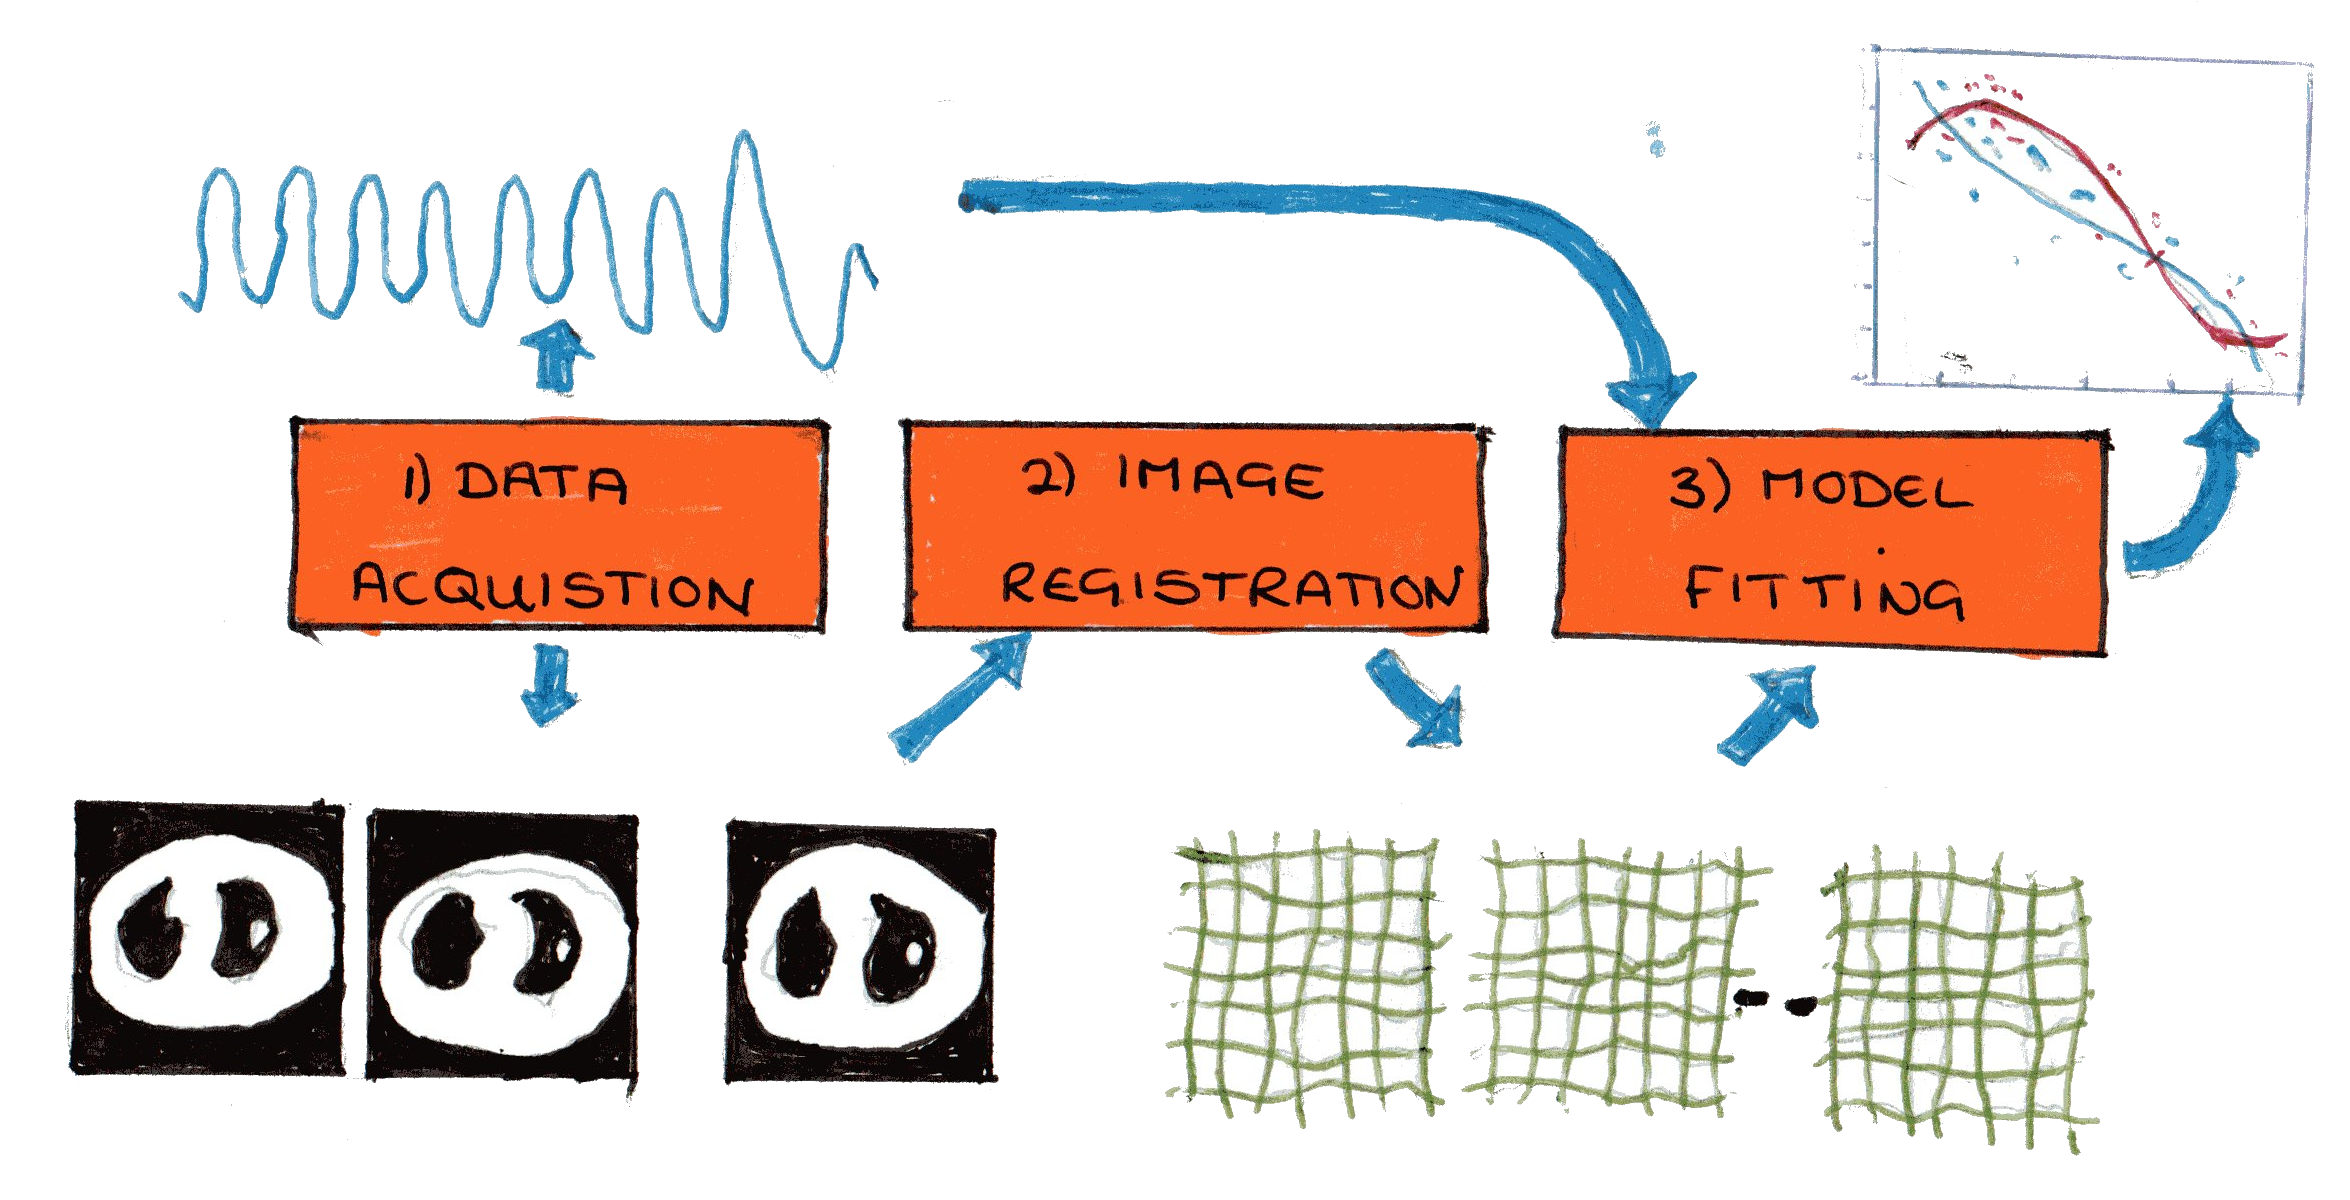
\includegraphics[width=1.0\linewidth]{figures/background_motion_model.png}
                        
                \captionsetup{singlelinecheck=false, justification=raggedright}
                \caption{Graphical representation of the process of \gls{MM}. On the left the initial data acquisition of both the data and the \gls{SS} can be seen. Then in the centre the data is taken and an image registration is applied to it. Then on the right it can be seen that the \gls{SS} is taken again and a \gls{RCM} is fit on it and the \gls{DVF} from image registration. In the top right a naive example of the \gls{2D} regression fit can be seen.} \label{fig:motion_modelling_motion_model}
            \end{figure}
            
            \gls{MM} offer an alternative solution to \gls{MC} when compared to vanilla co-registration of respiratory gated \gls{PET}. \gls{MM}, as with the \gls{RPM} discussed in \Fref{sec:external_devices}, are a technique borrowed from radiotherapy. \gls{MM} themselves attempt to relate the \gls{DVF} from, for instance, image registration to the \gls{SS} acquired for the data used to generate the \gls{DVF}. In this case a \gls{RCM} would be generated which is fit on all of the \gls{DVF}, from all of the data, related to all of the elements in the \gls{SS}, this can be seen in~\Fref{fig:motion_modelling_motion_model}~\boxcite{McClelland2013, McClelland2006, McClelland2014, McClelland2017}.
            
            There are four components required to perform \gls{MM}, these are; the data itself which is to be \gls{MC}, a \gls{SS} with an element for each of the pieces of data (the \gls{SS} can be \gls{ND}), the \gls{DVF} for each piece of data (for instance b-spline interpolated \gls{CPG} \gls{DVF}) and the \gls{RCM} linking the \gls{DVF} and \gls{SS}.
            
            An advantage of \gls{MM} over vanilla co-registration is that it allows for prediction of data not used to fit the \gls{RCM}, this advantage is particularly useful for radiotherapy. Here, data is acquired over some time on the machine used to perform radiotherapy on the patient on the day they are to receive radiotherapy. This allows for a \gls{RCM} to be fit on the data acquired with a \gls{SS} from, for instance, the \gls{RPM}. Then, as a dose is administered to the patient, from a linear accelerator, \gls{SS} can continue to be acquired and \gls{DVF} calculated using the \gls{RCM} in order to, in real time, change the trajectory of the linear accelerator to apply a dose only in the \gls{ROI}. The new \gls{SS} need not match any of the \gls{SS} used to generate the \gls{RCM} as the \gls{RCM} is a continuous model. This advantage could provide the functionality in \gls{PET} of calculating a \gls{RCM} while acquisition is still ongoing to be used for \gls{MC} during reconstruction. An additional advantage of \gls{MM} is that compared to vanilla co-registration it provides superior sensitivity to noise. this is because, while vanilla co-registration will register each individual volume together, regardless of how well that registration fits the underlying motion of the patient, \gls{MM} will then fit on top of, for instance, a registration, smoothing the effect of outliers and noise somewhat.
            
            \subsubsection{Respiratory Correspondence Model} \label{sec:respiratory_correspondence_model}
                \begin{figure}
                    \centering
                            
                    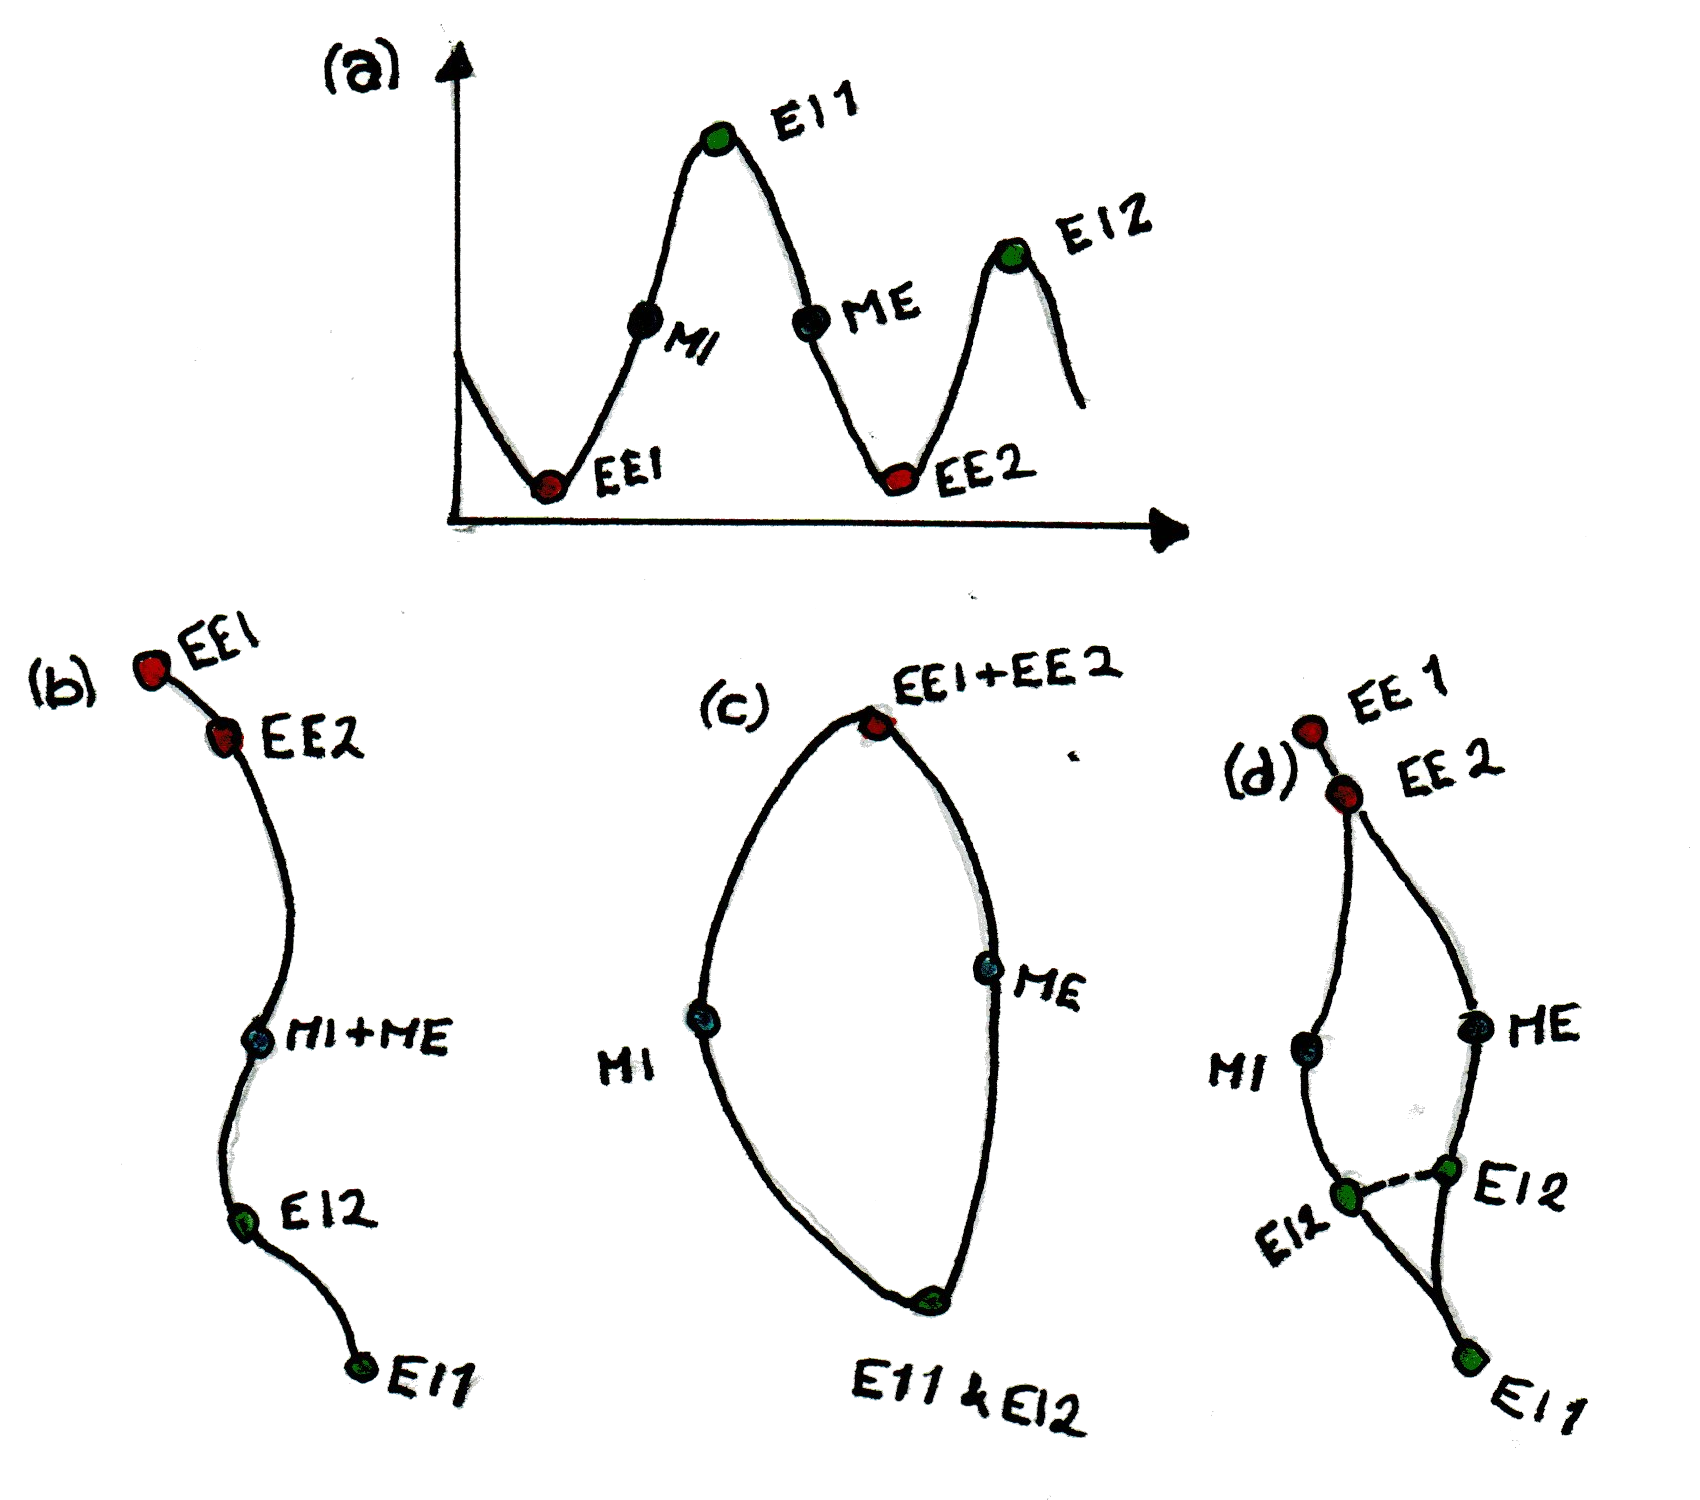
\includegraphics[width=1.0\linewidth]{figures/background_rcm.png}
                            
                    \captionsetup{singlelinecheck=false, justification=raggedright}
                    \caption{Graphical representation of . On the left .} \label{fig:motion_modelling_rcm}
                \end{figure}
                
        
        \subsection{Applying Motion Correction} \label{sec:applying_motion_correction}
            As discussed throughout this chapter, briefly in~\Fref{sec:respiratory_motion_challenges_in_combined_pet_ct_imaging} and~\Fref{sec:respiratory_gating}, there are a number of methods through which \gls{DVF} or \gls{MM} can be taken and the information gained through their acquisition can be applied to improving artefacts and image resolution from motion. These methods mostly fit into two different classes of \gls{MC} techniques, these are:
            
            \begin{itemize}
                \item Firstly, post-image reconstruction \gls{MC}. This class of \gls{MC} technique either takes the \gls{DVF} from image registration or the results of \gls{MM} and applies them after the \gls{PET} acquisition data has been reconstructed into images. Usually image registration is optimised in image space using an objective function such as \gls{MI} of \gls{MSE}, discussed in~\Fref{sec:image_registration}. An example of a post-image reconstruction \gls{MC} technique would be performing respiratory gating, reconstructing the gated volumes and then registering and summing all gates together, this was discussed briefly in~\Fref{sec:respiratory_motion_challenges_in_combined_pet_ct_imaging}. This method has the advantage that it is relatively simple to implement, each section of reconstruction and \gls{MC} is separate and sequential. Because of this each optimisation is more likely to converge to a result without having issues such as, the scale of each optimisation being different and requiring preconditioning or each iterative update being in a significantly different direction. However, because \gls{MC} is performed post-image reconstruction then this joint information cannot be taken into account during image reconstruction to aid with things such as aligning the \gls{mu-map} or improving convergence.
                
                \item Secondly, iterative image reconstruction and \gls{MC}. This class of \gls{MC} technique take the optimisation for image reconstruction and either image registration or \gls{MM} and iterates between them. An example of an iterative image reconstruction and \gls{MC} technique would be \gls{ML} joint image reconstruction and motion estimation as briefly discussed in~\Fref{sec:respiratory_motion_challenges_in_combined_pet_ct_imaging}. Here, a \gls{ML} image reconstruction is iteratively optimised for in conjunction with a motion estimate which is applied to both the estimated activity volume and the \gls{mu-map} in order to find a \gls{MC} activity volume which corresponds to the position of the \gls{mu-map} at every gate~\boxcite{Bousse2016}. An advantage of this technique is that between every iteration, from image reconstruction to \gls{MC}, the improvement of the accuracy of the activity distribution aids in fitting a \gls{MC} which then inversely can improve the resolution of the reconstruction. Eventually this can lead to an improved result over post-image reconstruction \gls{MC}. However, because this class of applied \gls{MC} involves a higher level of complexity, from integrating the reconstruction and \gls{MC}, it can prove more difficult to implement well and can increase computation time of the algorithm. In some cases it is possible to attempt to optimise for both the reconstructed image and image registration or \gls{MM} simultaneously, in this case it would be a simultaneous image reconstruction and \gls{MC} technique.
            \end{itemize}
    
    \longsection{Machine Learning for PET}{sec:machine_learning_for_pet}
        
        
        \subsection{Machine Learning Concepts} \label{sec:machine_learning_concepts}
            
            
            \subsubsection{Neural Network Architecture} \label{sec:neural_network_architecture}
                
                
            \subsubsection{Activation Function} \label{sec:activation_function}
                
            
            \subsubsection{Regularisation} \label{sec:regularisation}
                
        
        % \subsection{Machine Learning for PET Image Reconstruction} \label{sec:machine_learning_for_pet_image_reconstruction}
            % might want to mention this?
            
        
        \subsection{Machine Learning for Motion Correction} \label{sec:machine_learning_for_motion_correction}
            

    \chapter{Results} \label{results}
    \blindtext
    
    \longsection{Impact of TOF on Respiratory Motion Modelling using NAC PET}{impact_of_tof_on_respiratory_motion_modelling_using_nac_pet}
        \gls{RM} reduces image quality in \gls{PET}. Unless gated \gls{CT} or \gls{MR} data are available, \gls{MC} relies on registration of the \gls{PET} data. To avoid mis-registration due to attenuation mismatches, most existing methods rely on pair wise registration of \gls{NAC} \gls{PET} volumes. This is a challenging problem due to the low contrast and high noise of these volumes. This section investigates the possibility of using \gls{MM}s for respiratory \gls{MC} in \gls{PET}, and in particular whether incorporating \gls{TOF} information increases the accuracy of the \gls{MM}s derived from the \gls{NAC} reconstructed images. \gls{XCAT} phantom simulations are used for $1$ bed position with a \gls{FOV} including the base of the lungs and the diaphragm. A \gls{TOF} resolution of $375$ picoseconds is used. \gls{NAC} images are reconstructed using \gls{OSEM} and used as input for \gls{MM} estimation. Different \gls{MM}s are compared using the original \gls{XCAT} input volumes. The results indicate that \gls{TOF} improves the accuracy of the \gls{MM} considerably.
        
        \subsection{Introduction} \label{impact_of_tof_on_respiratory_motion_modelling_using_nac_pet_introduction}
        \gls{RM} causes artefacts and loss of resolution in the thoracic region in \gls{PET}~\boxcite{Nehmeh2008}. Many methods have been proposed to correct for \gls{RM}, usually involving registration between a reference volume and a set of volumes in different positions in the respiratory cycle obtained by gating~\boxcite{Oliveira2014}. However, such pair wise registration is sensitive to noise. It also does not allow prediction of the respiratory state for data not used to estimate the motion, for instance, to be used for real time \gls{MC}. Surrogate driven \gls{MM}s attempt to overcome these deficiencies by relating the motion in the data to a number of \gls{SS}s~\boxcite{McClelland2013}. The model outputs a transformation or \gls{DF} for every value of the \gls{SS}s. \gls{MM}s are calculated on a series of either time or gating based volumes.

        The benefits of using \gls{AC} \gls{PET} for \gls{IR} are unclear. If images are reconstructed using a static \gls{mu-map}, then artefacts caused by the misalignment between the activity distribution and the \gls{mu-map} would hamper \gls{IR}. It could therefore be advantageous to estimate motion on \gls{NAC} images~\boxcite{WenjiaBai2011}. However, contrast may be too low to calculate an accurate \gls{MM} and artefacts associated with the mismatch between the acquisition and system model could also obscure the underlying motion. 
        
        In the absence of \gls{TOF}, there is no information on the activity position along the \gls{LOR} and \gls{NAC} reconstructions have high intensity near the surface and low contrast in the internal part of the body. In \gls{TOF}, the time information constrains the activity position along the \gls{LOR} changing the nature and extent of the artefacts associated with \gls{NAC} as well as changing noise properties~\boxcite{Ter-Pogossian1981}.
        
        The aim of this section is to investigate whether \gls{TOF} can sufficiently increase the contrast and lower the noise of \gls{NAC} images to facilitate the calculation of accurate \gls{MM}s.
        
        \subsection{Methods} \label{impact_of_tof_on_respiratory_motion_modelling_using_nac_pet_methods}
            \subsubsection{XCAT Image Generation} \label{impact_of_tof_on_respiratory_motion_modelling_using_nac_pet_methods_xcat_image_generation}
                \gls{XCAT}~\boxcite{Segars2010} was used to generate $6$ volumes over a linear $5$ second breathing cycle, with $1$ volume at full expiration at the beginning of the cycle and $1$ volume at full expiration at the end of the cycle and using settings for the extent of \gls{AP} and \gls{SI} motion. Activity concentrations were derived from a static \gls{FDG} patient scan. The \gls{FOV} included the base of the lungs, diaphragm and the top of the liver with a $40$ millimetre diameter spherical lesion placed in the right lung.
            
            \subsubsection{PET Data Simulation} \label{impact_of_tof_on_respiratory_motion_modelling_using_nac_pet_methods_pet_data_simulation}
                \gls{PET} acquisitions were simulated using \gls{STIR}~\boxcite{Thielemans2012},~\boxcite{Efthimiou2018} through \gls{SIRF}~\boxcite{ovtchinnikov2019SIRFSynergisticImage,ovtchinnikov_evgueni_2019_3548719} to forward project the input data to sinograms using the geometry of a GE Discovery 710 and, where relevant, a \gls{TOF} resolution of $375$ picoseconds similar to the GE Signa \gls{PET}/\gls{MR} (using \gls{TOF} mashing to reduce computation time resulting in $13$ \gls{TOF} time bins of size $376.5$ picoseconds). Attenuation was included in the simulation using the relevant \gls{mu-map} generated by \gls{XCAT}. Scatter and randoms were not taken into account in the simulation. Multiple noise realisations were generated to simulate an acquisition as if it had been gated into $6$ bins over an acquisition of $120$ seconds, emulating a standard single bed position acquisition. 
            
            \subsubsection{Image Reconstruction} \label{impact_of_tof_on_respiratory_motion_modelling_using_nac_pet_methods_image_reconstruction}
                Data were reconstructed without attenuation correction using \gls{OSEM} with $2$ full iterations and $24$ subsets~\boxcite{Hudson1994}. Volumes were post filtered using a Gaussian blurring with a kernel size of $6.4$ millimetre \gls{FWHM}.
            
            \subsubsection{\gls{MM} Estimation} \label{impact_of_tof_on_respiratory_motion_modelling_using_nac_pet_methods_motion_model_estimation}
                \gls{3D} b-splines were used to model spatial deformations with the corresponding warping operation denoted as $\mathbf{W}(\mathbf{\alpha}_t)$, with $\mathbf{\alpha}_t$ a vector with B-spline coefficients at time $t$. The breathing \gls{SS}s $\mathbf{s}$ contained two components, the \gls{AP} and \gls{SI} motion signals used by \gls{XCAT}. Following~\boxcite{McClelland2017} a direct correspondence \gls{MM} was used where the b-spline coefficients at time $t$ are expressed as a linear combination of the $2$ \gls{SS}s, $s_{1,t}$ and $s_{2,t}$:
            
                \begin{equation}
                    \forall t \in [[1,n_t]], \alpha_{k,t} := R_{1,k} s_{1,t} + R_{2,k} s_{2,t} + R_{3,k}
                \end{equation}
                
                \noindent where $\alpha_{k,t}$ is the \gls{3D} b spline coefficient for node $k$ at time point $t$, and $R_{i,k}$ are the model parameters.
            
                A generalised framework unifying \gls{IR} and respiratory \gls{MM}s, NiftyRegResp, was used to estimate the \gls{RCM}s, which are the object that take in a \gls{SS} value and a volume and warp the volume based on the value of the \gls{SS} object, of the \gls{MM}, using \gls{SSD} as an objective function~\boxcite{McClelland2017}.
                
            \subsection{Evaluation} \label{impact_of_tof_on_respiratory_motion_modelling_using_nac_pet_methods_evaluation}
                We compared $3$ \gls{RCM}s, calculated from the \gls{PET} \gls{XCAT} volumes (gold standard), \gls{NTOF} \gls{NAC} reconstructions and \gls{TOF} \gls{NAC} reconstructions. To test the accuracy of the \gls{RCM}s, the $3$ models were used to warp the \gls{PET} volume generated by \gls{XCAT} at the mean breathing position to the position at each gate. These estimated volumes were then compared to the original \gls{XCAT} input volumes. Difference volumes were obtained by subtracting the original \gls{XCAT} volume $\mathbf{f}_t$ and warped volumes $\mathbf{W}(\alpha_t) \mathbf{f}_\mathrm{ref}$ at the same gate. \gls{MAPE} were computed from these difference images. \gls{MAPE} is expressed as:
                
                \begin{equation}
                   % M := \frac{\frac{\sum_{n}^{1}\abs{g - e}}{n}}{\frac{\sum_{n}^{1}g}{n}} \times 100
                   M:= \frac{\frac{1}{n}\sum_{n}\mid e_n - g_n \mid}{\frac{1}{n}\sum_{n}g_n} \times 100
                \end{equation}
                
                \noindent where $M$ is the result of applying \gls{MAPE} to $e$ the estimated volumes with respect to $g$ the ground truth volumes for $n$ the number of volumes.
                
                In addition, the \gls{COM} of the lesion was also tracked over the $6$ gates, by warping a volume only including the lesion in the reference position as above, and then computing the \gls{COM}.
            
        \subsection{Results} \label{impact_of_tof_on_respiratory_motion_modelling_using_nac_pet_results}
            \begin{figure*}
                \centering
                
                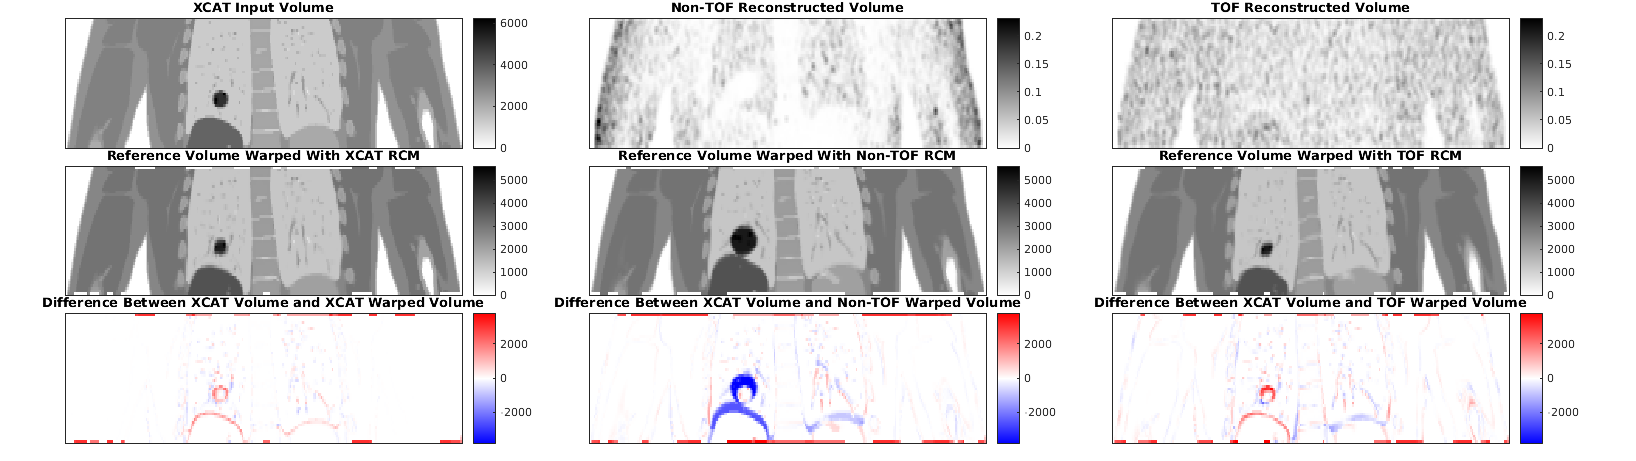
\includegraphics[width=1.0\linewidth]{figures/output.png}
                
                \captionsetup{singlelinecheck=false, justification=raggedright}
                \caption{All volumes correspond to end inhalation. First row from left to right: \gls{XCAT} \gls{PET} data, \gls{NAC} \gls{NTOF} reconstructed data and \gls{NAC} \gls{TOF} reconstructed data. Second row: \gls{RCM} applied to mean position \gls{XCAT} data with \gls{RCM} derived from \gls{XCAT} \gls{PET} data (left), \gls{NAC} \gls{NTOF} (middle) and \gls{NAC} \gls{TOF} (right) volumes. Colour map ranges are consistent for all images on this row. The third row from left to right: The difference between the estimated volumes from the second row with the \gls{XCAT} end-inhalation volume. Colour map ranges are consistent for all images on this row.} \label{fig:output}
            \end{figure*}
            
            \begin{table}
                \centering
                
                \captionsetup{singlelinecheck=false, justification=raggedright}
                \caption{Comparison of the \gls{MAPE} between the ground truth data and the volumes estimated from the \gls{XCAT} based \gls{RCM}, the volumes estimated from the \gls{NAC} \gls{NTOF} based \gls{RCM} and the volumes estimated from the \gls{NAC} \gls{TOF} based \gls{RCM}.}
                
                \resizebox*{1.0\linewidth}{!}
                {
                    \begin{tabular}{||c|ccc||}
                        \hline
                        \textbf{\gls{MAPE}} & \textbf{XCAT} & \textbf{\gls{NTOF}} & \textbf{\gls{TOF}} \\
                        \hline
                        \textbf{$1$} & $1.95$ & $8.35$ & $4.18$ \\
                        \textbf{$2$} & $1.59$ & $1.61$ & $1.84$ \\
                        \textbf{$3$} & $2.06$ & $9.91$ & $5.23$ \\
                        \textbf{$4$} & $1.97$ & $6.15$ & $3.68$ \\
                        \textbf{$5$} & $1.65$ & $4.45$ & $2.52$ \\
                        \textbf{$6$} & $1.95$ & $8.35$ & $4.18$ \\
                        \hline
                        \textbf{Mean} & $1.86$ & $6.47$ & $3.60$ \\
                        \hline
                    \end{tabular}
                } \label{tab:mape}
            \end{table}
            
            \begin{figure}
                \centering
                
                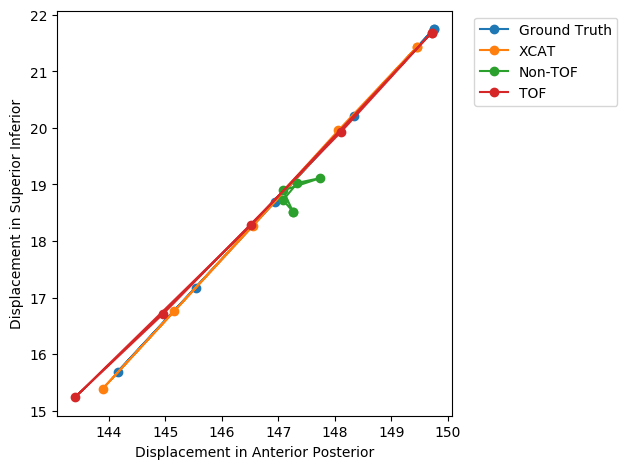
\includegraphics[width=1.0\linewidth]{figures/TOF.png}
                
                \captionsetup{singlelinecheck=false, justification=raggedright}
                \caption{The path of the \gls{COM} of the lesion. Horizontal (respectively vertical) axis corresponds to motion in the \gls{AP} (respectively \gls{SI}) direction over the six gates. Different curves denote \gls{COM} displacement for  ground truth data, the estimated data from the \gls{XCAT} based \gls{RCM}, the estimated data from the \gls{NAC} \gls{NTOF} based \gls{RCM} and the estimated data from the \gls{NAC} \gls{TOF} based \gls{RCM}.} \label{fig:com_graph}
            \end{figure}
            
             The reconstructed data, estimated volumes and difference can be seen in Figure~\ref{fig:output} and \gls{MAPE} are in Table~\ref{tab:mape}. The mean \gls{MAPE} was found to be lower for the \gls{NAC} \gls{TOF} data than for the \gls{NAC} \gls{NTOF}.
            
             \gls{COM} results can be seen in Figure~\ref{fig:com_graph}. The path of the \gls{NAC} \gls{TOF} data follows the ground truth path much closer than the \gls{NAC} \gls{NTOF} data, and is quite close to the gold standard \gls{XCAT}-derived motion.
            
        \subsection{Discussion and Conclusion} \label{impact_of_tof_on_respiratory_motion_modelling_using_nac_pet_discussion_and_conclusion}
            \gls{MM}s derived from \gls{NAC} \gls{TOF} volumes were found to be more robust than when using \gls{NAC} \gls{NTOF}, both visually and when comparing \gls{MAPE} and \gls{COM}. This was noticeable for the lung lesion in the thoracic cavity but also for other parts of the anatomy such as the liver. This is likely due to the improved image contrast of \gls{NAC} \gls{TOF} images.

            In the future, research will focus on investigating the robustness of the \gls{MM} estimation to different noise levels, acquisition duration and size of lesion.
    
    \longsection{Impact of TOF on Respiratory Motion Modelling using NAC PET: an Extension to Inter and Intra Respiratory Cycle Variation}{impact_of_tof_on_respiratory_motion_modelling_using_nac_pet_an_extension_to_inter_and_intra_respiratory_cycle_variation}
        \blindtext
        
        \subsection{Introduction} \label{impact_of_tof_on_respiratory_motion_modelling_using_nac_pet_an_extension_to_inter_and_intra_respiratory_cycle_variation_introduction}
        
        \subsection{Methods} \label{impact_of_tof_on_respiratory_motion_modelling_using_nac_pet_an_extension_to_inter_and_intra_respiratory_cycle_variation_methods}
            \blindtext
            
        \subsection{Results} \label{impact_of_tof_on_respiratory_motion_modelling_using_nac_pet_an_extension_to_inter_and_intra_respiratory_cycle_variation_results}
            \blindtext
            
        \subsection{Discussion and Conclusion} \label{impact_of_tof_on_respiratory_motion_modelling_using_nac_pet_an_extension_to_inter_and_intra_respiratory_cycle_variation_discussion_and_conclusion}
            \blindtext
    
    \longsection{Extension of Static PCA Based Data Driven Surrogate Signal Extraction to Dynamic PET}{extension_of_static_pca_based_data_driven_surrogate_signal_extraction_to_dynamic_pet}
        \blindtext
        
        \subsection{Introduction} \label{extension_of_static_pca_based_data_driven_surrogate_signal_extraction_to_dynamic_pet_introduction}
        
        \subsection{Methods} \label{extension_of_static_pca_based_data_driven_surrogate_signal_extraction_to_dynamic_pet_methods}
            \blindtext
            
        \subsection{Results} \label{extension_of_static_pca_based_data_driven_surrogate_signal_extraction_to_dynamic_pet_results}
            \blindtext
            
        \subsection{Discussion and Conclusion} \label{extension_of_static_pca_based_data_driven_surrogate_signal_extraction_to_dynamic_pet_discussion_and_conclusion}
            \blindtext
    
    \longsection{Feasibility of Neural Network Based Data Driven Surrogate Signal Extraction Methods for Dynamic PET}{feasibility_of_neural_network_based_data_driven_surrogate_signal_extraction_methods_for_dynamic_pet}
        \blindtext
        
        \subsection{Introduction} \label{feasibility_of_neural_network_based_data_driven_surrogate_signal_extraction_methods_for_dynamic_pet_introduction}
        
        \subsection{Methods} \label{feasibility_of_neural_network_based_data_driven_surrogate_signal_extraction_methods_for_dynamic_pet_methods}
            \blindtext
            
        \subsection{Results} \label{feasibility_of_neural_network_based_data_driven_surrogate_signal_extraction_methods_for_dynamic_pet_results}
            \blindtext
            
        \subsection{Discussion and Conclusion} \label{feasibility_of_neural_network_based_data_driven_surrogate_signal_extraction_methods_for_dynamic_pet_discussion_and_conclusion}
            \blindtext

    \chapter{Discussion and Conclusion} \label{discussion_and_conclusion}
    \blindtext
    
    \longsection{Future Work}{future_work}
        \blindtext
        
        \subsection{Gantt Chart} \label{gantt_chart}
            \blindtext

    % \addcontentsline{toc}{chapter}{Appendices}

\chapter{Appendices}
% The \appendix command resets the chapter counter, and changes the chapter numbering scheme to capital letters.
\appendix
\chapter{Appendix} \label{appendixlabel1}
    \blindtext
    
\chapter{Colophon} \label{appendixlabel3}
    \textit{This document was set in the Times Roman typeface using \LaTeX\ and Bib\TeX , composed with a text editor.}
 
    % You could separate these out into different files if you have
    %  particularly large appendices.
    
    % This line manually adds the Bibliography to the table of contents.
    % The fact that \include is the last thing before this ensures that it
    % is on a clear page, and adding it like this means that it doesn't
    % get a chapter or appendix number.
    \addcontentsline{toc}{chapter}{Bibliography}
    
    % Actually generates your bibliography.
    \printbibliography
    % All done. \o/
\end{document}
